\documentclass{article}
\usepackage{pgffor}
\usepackage{filecontents}
\usepackage{pdfpages }
\usepackage{graphicx} 
\usepackage{a4wide}
\usepackage{here} 
\usepackage{tabularx}
\usepackage[colorlinks]{hyperref}
\usepackage[german]{babel}
\usepackage[utf8]{inputenc}
\usepackage[T1]{fontenc}
\usepackage[3D]{movie15}
\usepackage{booktabs} 
\usepackage{eurosym}
\usepackage{verbatim}
\usepackage{amsmath}
\usepackage{textcomp}
\usepackage{caption}
\usepackage{setspace} 

\setcounter{tocdepth}{5}  % Ebenen für Aufnahme in das Inhaltsverzeichnis
\setcounter{secnumdepth}{4}  % Ebenen für Nummerierung


\begin{document}


% Titelseite
\title{CanSat 2015 Team Gamma Dokumentation}
\date{\today}
\author{Alexander Brennecke \and Till Schlechtweg \and Marc Huisinga \and Robin Bley \and Steffen Wißmann \and Alexander Feldmann \and Kevin Neumeyer}
\maketitle

\newpage

\tableofcontents
\newpage

% Import der Einleitung
\section{Einleitung}

Diese Dokumentation dokumentiert die Arbeit an dem Dosensatelliten ``Apollo 13'' und die Entwicklung einer Bodenstation zur Datenverarbeitung der Daten des Satelliten im Rahmen des Deutschen CanSat-Wettbewerbs 2015 und des P5-Projekts der Europaschule SZII Utbremen.

\subsection{Teamorganisation und Aufgabenverteilung }

Das gesamte Team besteht aus sieben Schülern und zwei betreuenden Lehrern. Die sieben Schüler sind intern in mehrere kleinere Teams aufgeteilt. Innerhalb der Teams ist kein Teammitglied vollkommen an seine Aufgaben gebunden, da uns ein guter Austausch und eine hervorragende Zusammenarbeit zwischen den einzeln Teammitgliedern und Teams wichtig ist. Die Arbeiten der Gruppen und der einzelnen Personen werden im Folgenden erläutert:

\begin{itemize}
\item Das Hardware-Team besteht aus drei Personen, welche sich um den Bau des Satelliten selber, das Design und den Bau der Dose sowie die Programmierung des Mikrocontrollers kümmern. Zu diesem Team zählen folgende Personen:
\begin {description}
\item [Alexander Brennecke] ist verantwortlich für das Design der Dose. Dazu zählt die Konstruktion der eigentlichen Dose und die Anordnung der Sensoren im Inneren der Dose.

\item [Till Schlechtweg] ist verantwortlich für die Funktionalität des Mikrocontrollers und der ausgewählten Sensoren.

\item [Steffen Wißmann] ist verantwortlich für die Übertragung der Daten zur Bodenstation und den Programmcode des Mikrocontrollers.
\end {description}
\item Das Software-Team besteht aus vier Personen, welche sich um das Programmieren der Bodenstation und der Android-Applikation kümmern. Allgemein gilt für alle Personen dieser Gruppe, dass die Grenzen der Zuständigkeitsbereiche der verschiedenen Personen verfließen, wobei jede Person allerdings noch ein gewisses Spezialgebiet besitzt. Dieses Team besteht aus folgenden Personen:
\begin {description}
\item [Robin Bley] ist verantwortlich für das Implementieren der Datenverarbeitung der Bodenstation und für das Testen von kritischen Bereichen innerhalb der Datenverarbeitung.

\item [Alexander Feldmann] ist verantwortlich für die Entwicklung der Android-Applikation.

\item [Marc Huisinga] ist ebenfalls verantwortlich für das Implementieren der Datenverarbeitung der Bodenstation, für die Entwicklung der Datenvisualisierungskomponenten und für die Architektur der Datenverarbeitung.

\item [Kevin Neumeyer] ist verantwortlich für die zusammenführende Architektur der Bodenstation, die grafische Umgebung und die Administration der Software-Repositories.
\end {description}
\item Zudem gibt es ein Team, bestehend aus Alexander Brennecke und Till Schlechtweg, welches sich um die Organisation, die Kommunikation mit Sponsoren und die Öffentlichkeitsarbeit kümmert.

\item Betreut wird das Projekt durch zwei Lehrer unserer Schule:
\begin{description}
\item [Mathematiklehrer Harm Hörnlein-Roboom], welcher als Ansprechpartner für die Software-Gruppe zur Verfügung steht.
\item [Physiklehrer Frank Marshall], welcher als Ansprechpartner für die Hardware-Gruppe und den CanSat-Wettbewerb zur Verfügung steht.
\end{description}

\end{itemize}

Zusätzlich zu diesen etwaigen Zuständigkeitsbereichen haben wir die Arbeit innerhalb der Teilprojekte in verschiedene Tickets aufgeteilt. Die Tickets wurden über die gesamte Arbeitszeit, je nach Bedarf, wie folgt, verteilt und bearbeitet:

\begin{table}[H]
	\centering
	\begin{tabular}{rl}
		\toprule
		\textbf{Person} & \textbf{Aufgaben} \\
		\midrule
		Robin Bley & Verbindungsschnittstelle zum Smartphone \\
		 & Alle automatisierten Softwaretests \\
		 & Parsen von Daten\\
		 & Loggen von Daten \\
		 & Mehrmaliges Erneuern aller Export- und Importkomponenten\\
		 & Alle Exportkomponenten bis auf KML \\
		 & Alle Importkomponenten\\
		 & Mehrmaliges Erneuern der automatisierten Tests\\
		 & Bearbeitung des Brandings\\
		Alexander Brennecke & Ticket \\
		Alexander Feldmann & Fallschirm \\
		 & Livegraph (Android-App) \\
		 & Balkendiagramm (Android-App) \\
		 & Optionen (Android-App) \\
		 & Menü (Android-App) \\
		 & Schnittstelle zur Bodenstation (Android-App) \\
		 & Debug-Stream (Android-App) \\
		Marc Huisinga & Datenempfang über serielles Interface \\
		 & Debug-Datenstream \\
		 & Datenweiterleitung an Endkomponenten \\
		 & Datenabflachung und Behandlung fehlerhafter Daten \\
		 & Weltkartenvisualisierung \\
		 & KML-Exporter \\
		 & Textstream-Visualisierung \\
		 & Tabellenvisualisierung \\
		 & Pflegen der Code-Dokumentation \\
		 & Refactoring der Input-Pipeline \\
		Kevin Neumeyer & Verarbeiten von Konfigurationsdateien \\
		 & Zusammenführen der InputPipeline als Service \\
		 & Dynamischer Zusammenbau von Datenquellen \\
		 & Zusammenführen von Import- und Export-Komponenten \\
		 & Satellitenmanagement \\
		 & Modulrefactoring \\
		 & Verwaltung des Repositories \\
		 & Graphische Benutzeroberfläche \\
		 & Graphenvisualisierung \\
		Till Schlechtweg & Ticket \\
		Steffen Wißmann & Ticket \\
		\bottomrule
	\end{tabular}
\end{table}

Die Dokumentation und die Präsentation wurden ebenfalls von unterschiedlichen Personen geschrieben. Folgende Anteile wurden wie folgt aufgeteilt:

\begin{table}[H]
	\centering
	\begin{tabular}{rl}
		\toprule
		\textbf{Person} & \textbf{Bereiche} \\
		\midrule
		Robin Bley & Reflexion der Softwaregruppe \\
		 & 3.1.6 Nutzeranleitung \\
		 & 3.1.3.3 Features \\
		 & 3.1.7 Realisierung der Desktopapplikation \\
		 & 3.1.5 Tests \\
		 & Teilkorrektur der Dokumentation \\
		 & Großteil der Präsentation \\
		Alexander Brennecke & Bereich \\
		Alexander Feldmann & 2.5 Bergungssystem \\
		 & 2.6 Aufgetretene Probleme \\
		 & 2.7 Testkonzept \\
		 & 3.2 Android-Applikation \\
		 & 4.1.2 Zeitplanung der Software-Gruppe (App) \\
		 & 7.2.2 Reflexion Android-Applikation \\
		 & Fallschirms- und Android-App-Folien der Präsentation \\
		Marc Huisinga & 3.1.1 Überblick \\
		 & 3.1.2 Verwendete Komponenten \\
		 & 3.1.4 Architektur \\
		 & 4.1.2 Zeitplanung der Software-Gruppe (Desktopapplikation) \\
		 & 7.2.1 Desktopapplikation \\
		 & Komplette Korrektur der Dokumentation \\
		 & Planungsfolien der Präsentation \\
		Kevin Neumeyer & 3.1.3.1 Nutzerfreundlichkeit \\
		 & 3.1.3.2 Erweiterbarkeit \\
		Till Schlechtweg & Bereich \\
		Steffen Wißmann & Bereich \\
		\bottomrule
	\end{tabular}
\end{table}

Die Arbeit an dem Projekt findet zum größten Teil wöchentlich am Dienstag und Mittwoch Nachmittag in den Laboren unserer Schule statt. Die Labore sind mit diversen Werkzeugen ausgestattet, sodass sowohl die Software- als auch die Hardware-Gruppe dort problemlos arbeiten können. Zusätzlich zu diesen vier bis acht Stunden pro Woche kommen fünf Projekttage, welche uns von der Schule breitgestellt wurden. Natürlich arbeitet jedes Teammitglied auch außerhalb dieser Treffen an seinem Fachgebiet, soweit dies möglich ist. Zusätzlich gibt es auch immer wieder Treffen mit externen Unterstützungen, oder Arbeitszeit in der Schule, wenn Vertretungs- oder Mitbetreuungsunterricht stattfindet.

\subsubsection{Stärken des Teams}
Die große Stärke des Teams ist es, dass es auch schon vor diesem Projekt existiert hat und sich somit sehr gut kennt. Die Teilnahme am Europäischen CanSat Wettbewerb 2014 hat dazu geführt, dass jedes Teammitglied gewisse Vorkenntnisse mitbringt. Ebenfalls von Vorteil ist, dass jedes Teammitglied durch unsere schulische Ausbildung genügend Erfahrung hat, um auch außerhalb seines Fachgebietes unterstützend tätig zu sein. Zudem ist die Arbeits- und Leistungsbereitschaft der meisten Teammitglieder überdurchschnittlich gut.

\subsubsection{Verbesserungsbereiche des Teams}
Der größte Verbesserungsbereich des Teams liegt ganz klar im Zeitmanagement. Für viele Aufgaben wird zu wenig Zeit eingeplant. Oft kommt es auch vor, dass der Schwerpunkt der Arbeit auf Dingen liegt, welche nicht höchst priorisiert sind und somit Zeit beanspruchen, welche an anderen Stellen dringender benötigt würde. Ebenfalls problematisch ist, dass die meisten Teammitglieder gerne neue Technologien oder Praktiken ausprobieren wollen. Dieses Interesse ist zwar löblich und für die Einzelperson sehr lehrreich, jedoch kommt es bei neuen Technologien und Praktiken oft zu Problemen, die man bei bereits bekannten deutlich schneller lösen könnte.

\subsection{Missionsziel}
Die Idee hinter dem gesamten Projekts bezieht sich auf die extreme Umweltbelastung und ihre Folgen für den menschlichen Körper. Ausschlaggebend für diese Idee ist ein Zeitungsartikel der Zeit, welcher über eine drohende Klage der EU-Kommission in Brüssel berichtet. (vgl. Die Zeit, 24.10.2014). Die Klage richtet sich gegen Deutschland, da die deutsche Bundesregierung bisher zu wenig Aufwand betreibt, um die Feinstaubkonzentration in der Luft zu reduzieren. Wir möchten diesen Aspekt aufgreifen und Messungen durchführen um die tatsächlichen Werte zu bestimmen. Der CanSat Wettbewerb eignet sich optimal dazu, da er uns die Möglichkeit bietet, die Messungen nicht nur auf dem Boden, sondern auch in verschiedenen Schichten der Atmosphäre durchzuführen. Feinstäube stehen in Verdacht, Krankheiten wie Asthma, Herz-Kreislauf-Beschwerden und Krebs zu begünstigen.

Da der menschliche Körper nicht nur durch Feinstaub belastet wird, haben wir uns entschlossen, auch die Intensität der UV-Strahlung, welche die Hauptursache für Hautkrebserkrankungen ist, zu messen. Zusätzlich soll auch der Ozonwert bestimmt werden, da Ozon bereits in geringen Konzentrationen gesundheitsschädlich ist und zu Reizungen der Atemwege führen kann.

Für sich genommen ist jede dieser drei Größen schädlich für den Menschen. Im Zuge des Projektes wollen wir jedoch versuchen herauszufinden, ob es einen Zusammenhang zwischen ihnen gibt. Beispielsweise ist herauszufinden, ob ein höherer Ozongehalt gleichzeitig einen niedrigeren Feinstaubgehalt mit sich bringt.

Zusätzlich zum Bau des Messsystems im CanSat, ist es unser Ziel, eine einwandfreie Verarbeitung, Analyse und Präsentation der gemessenen Werte zu erzielen. Um dies zu garantieren, programmieren wir ein eigenes Analysetool. Dieses Tool ermöglicht es uns, die gemessenen Werte während des Fluges des Satelliten auszuwerten. Die Werte sollen dabei anschaulich und in Abhängigkeit zueinander dargestellt werden. Die Bodenstation soll zusätzlich darauf ausgelegt sein, nicht nur unseren Satelliten zu unterstützen. Viel mehr soll das Analysetool auch anderen CanSat-Missionen eine Plattform bieten, auf der die gemessenen Daten ausgewertet werden können.

Um die Daten auch mobil verfügbar zu haben, möchten wir eine Android Applikation bereitstellen. Diese Applikation soll vorerst nur für unser Projekt optimiert sein, bei Erfolg jedoch auch die Werte anderen Teams anzeigen können.

\subsection{Praktischer Nutzen für den Auftraggeber}
Die Ausrichter des Wettbewerbes, welche in unserem Projekt als Auftraggeber angesehen werden, können aus unserem Projekt wahrscheinlich relativ wenig praktischen Nutzen ziehen. Der Wettbewerb, im Allgemeinen, bietet den Veranstaltern jedoch mehrere Möglichkeiten: Zum einen können dadurch mehr Jugendliche für die Bereiche Raumfahrt, Elektrotechnik, Informatik und Physik begeistert werden. Zum anderen kann es auch möglich sein, dass Mitglieder der Jury, welche meist in einem der gerade genannten Fachbereiche tätig sind, Lösungsansätze für Probleme der Wissenschaft in einem der Projekte wiederfinden. Ein weiterer praktischer Nutzen ist, dass unsere Bodenstation theoretisch in den folgenden Jahren den anderen Teams zur Verfügung gestellt werden kann, um die gemessenen Daten auszuwerten.



% Import der Hardware Doku
\section{Beschreibung des CANSAT}


% Blockdiagramm (irgendjemand)
\subsection{Missionsüberblick}
Wir haben uns für den Satelliten überlegt, dass dieser so weit wie möglich individuell sein sollte. Daher greifen wir nicht auf das, vom Wettbewerb bereitgestellte T-Minus CanSat Kit zurück. Stattdessen haben wir uns im Detail überlegt, welche Sensoren unseren Erwartungen entsprechen und wie wir diese bestmöglich innerhalb der Dose platzieren können. Zusätzlich möchten wir nicht auf eine Cola-Dose als Hülle zurück greifen, sondern möchten auch hier unser eigenes Design erschaffen.

% 3D Skizze, Erklärung der einzelnen Bestandteile (Alexander B.)
\subsection{Mechanisches und Strukturdesign}

Wir haben den CanSat in drei Komponenten aufgeteilt: Die Hülle, die Innenwand und die Sensorik Platine. Diese drei Komponenten bilden den Hauptbestandteil des CanSats und haben maßgeblich zu dem mechanischen und strukturellem Design beigetragen. Im nachfolgenden wird kurz auf jeden dieser Komponenten eingegangen und die exakte Funktion im Zusammenhang erklärt.

\subsubsection{Die Hülle}
Wir haben uns dazu entschieden, die äußere Hülle aus GFK (Glasfaser verstärkter Kunststoff) zu fertigen. Dieses hat die Eigenschaften, dass er bei einem sehr geringen Gewicht, und bei einer geringen Wandstärke trotzdem eine gewisse Stabilität aufweißt. Aus dem GFK haben wir eine Röhre mit einem Innendurchmesser von 31,5 mm und einem Außendurchmesser von 33,5 mm laminiert. Diese Röhre wurde auf eine Länge von 111 mm gekürzt und gefeilt. Um die Röhre oben und unten zu verschließen haben wir uns bei Thyssen Krupp System Engineering zwei Aluminium Deckel fräsen lassen. Diese haben uns ebenfalls durch ihr geringes Gewicht und ihre hohe Stabilität überzeugt.

\subsubsection{Innenwand}
Um die Elektronik innerhalb der Hülle zu platzieren und zu befestigen haben wir uns dazu entschieden eine Wand anzufertigen. Diese Wand teilt die Hülle mittig und bietet so auf beiden Seiten Platz um unser Mikrocontroller Board und unsere Sensorik Platine zu befestigen. Beide Bauteile werden mittels vier Gewindestangen an der Wand befestigt. Durch die Technik des 3D-Druckens ist es möglich der Wand ein sehr geringes Gewicht bei einer verhältnismäßig hohen Stabilität zu verleihen. Zusätzlich gibt es uns die Möglichkeit die Wand millimetergenau zu gestalten. \\
Am unteren Ende der Wand befindet sich eine Aushöhlung, sowie ein Fuß. Diese ist zum einen dafür da um den Sharp Feinstaub Sensor zu befestigen. Zum anderen gibt der Fuß der Wand und somit dem gesamten Satelliten eine gewisse Stabilität. Der Fuß besitzt auf der einen Seite der Wand Bohrungen. Diese Bohrungen werden verwendet um die Aluminiumdeckel an der Wand zu befestigen. An der oberen Seite der Wand befinden sich ebenfalls solche Bohrungen um den oberen Deckel der Hülle zu befestigen. Da der Feinstaubsensor einen Luftzug benötigt befindet sich ein Durchlass innerhalb der Wand. Um das Mikrocontroller Board mit der Sensorik Platine zu verbinden existiert ein Fenster in der Mitte der Wand. Um die Sensorik Platine und das Mikrocontroller Board an der Wand zu befestigen existieren vier Bohrungen.

\subsubsection{Die Sensorik Platine}
Die Sensorik Platine ist eine von uns geätzte Platine, welche mit unseren Sensoren bestückt ist. Es gibt mehrere positive Aspekte, die eine eigene Platine mit sich bringt. Zum einen bietet sie eine stabile Plattform für die Befestigung der Sensoren. Zum anderen sparen wir uns dadurch eine Menge Kabel, welche deutlich störanfälliger sind als eine Platine. Die Platine hat an den entsprechenden Stellen Bohrungen um sie mit der Zwischenwand und dem Mikrokontrollboard zu verbinden. Die Platine bietet Platz für folgende Module:

\begin{itemize}
	\item BMP108 Drucksensor: Misst den Luftdruck und gibt diesen, sowie die daraus berechnete Höhe zurück
	\item Sparkfun UV Sensor: Misst die Intensität des Spektrums 270-380 nm, welches dem UVA und UVB Spektrum entspricht
	\item TMP006 Infrarot Temperatursensor: Misst die Temperatur eines dünnen Aluminiumstückes in der Außenwand 
	\item Adafruit Ultimate GPS: Bestimmt die aktuelle Position sowie die Höhe
	\item APC220 Transceiver Modul: Sendet die Daten als JSON String zur Bodenstation
	\item Steckplatz zum Anschluss des Sharp Feinstaub Sensors: Misst den Anteil der Partikel, welche kleiner als 10 \textmu m sind
	\item Steckplatz zum Anschluss an das Mikrokontrollerdboard: Bildet die Schnittstelle zwischen BeagleBone und Senorik Platine
\end{itemize}

\subsubsection {Fachliche Grundlage}
Um die 3D gedruckte Wand zu erzeugen wurde die 3D Moddelierungssoftware \href{http://www.sketchup.com/de} {Sketchup} von Google verwendet. Sketchup bietet die Möglichkeit vergleichsweiße einfach 3D Modelle zu zeichnen. Um dies zu tun muss klar sein, welche Objekte gezeichnet werden sollen. Diese Objekte müssen vermessen und innerhalb von Sketchup gezeichnet werden. Dies erfordert die Kentniss über gewisse mathematische Methoden zur Berechnung von Kreisen, Flächen und Körpern. Die meisten 3D-Drucker benötigen Datein des Types .stl, welche in Sketchup mit einem Plugin erzeugt werden können.
Zum fertigen von GFK Komponenten wird ein Körper benötigt, auf welchen das GFK laminiert werden kann. In unserem Fall ist dieser Körper zylindrisch, mit einem Durchmesser von 31,5 mm, und aus Aluminium gefräst. \\
Um die Platine zu erstellen wurde die Design Software \href{http://www.cadsoft.de/eagle-pcb-design-software/} {Eagle PCB} verwendet. Eagle bietet die Möglichkeit sowohl Schaltpläne als auch das entsprechende Layout zu erstellen. Im Anschluss wurde die Platine, mit Hilfe und Mitteln des Hackerspace Bremen e.V. geätzt.



% Elektrisches Vorgehen, Schaltplan, Funkverbindung (Till)
\subsection{Elektrische Konstruktion}



\subsubsection{Fachliche Grundlagen}
\paragraph{Embedded System}
Ein Embedded System ist in unserem Fall der BeagleBone mithilfe vom ARM Cortex-A6 mit 1Ghz, ist ein leich modifizierte linux kernel mit Frontend installiert, dass liebevoll Angstrom genannt wurde. Um ein paar andere Beispiele für ein eingebettetes System sind etwa ein Smart TV oder ein Router, beide haben eine Art eingebettetes System, dass immer öfter auf dem Linux Kernel basiert und je nach Anwendung angepasst wurde. In unserem Fall unterstützt das BeagleBone verschiedene Technologien zum empfangen von Daten verschiedener Bauteile, wie etwa UART, I-2-C, SPI, Analog, Digital, PWM, Timer und PRU. Viele dieser Technologien sind in unserem Projekt nicht in Verwendung alle anderen Grundlagen sind unten beschrieben.

\paragraph{Transistor-Transistor-Logik}
5V werden immer als logische 1 bezeichnet, damit ist gemeint wenn der Sensor den höchsten Messwert erreicht gibt er eine Spannung von 5V. Ist dies nicht der Fall hat der Sensor eine andere Kennkurve die zum Beispiel bei 3.3V aufhört. Allgemein wird aber Transistor-Transistor-Logik genutzt, welche 5V als logische 1 und geerdet als logische 0 ansieht, es gibt natürlich Toleranzen, diese sind aber bei verschiedenen integrierte Schaltkreisen und Mikrokontrollern unterschiedlich.

\paragraph{Analog-to-Digital-Converter}
Andere Sensoren wie der UV-Sensor die nur über einen internen Wiederstand verfügen der sich, je nach Konzentration, an einer mathematischen Kurve orientierend, im Wert leicht verändert und dadurch die ankommende Spannung am jeweiligen Analog Pin ändert. Mithilfe eines Analog-to-Digital-Converter konvertieren wir das analoge Signal, zum Beispiel 5V, in das äquivalente digitale Signal mit der Auflösung von 12 Bits. \\

\[
2^{12} \quad = 4096
\]

\[
\frac{5V}{4096} = 0.001220703125 V
\] \\

Das bedeutet jeder 0.001220703125V kann dargestellt werden, wobei der Arduino Mega 2560 nur 10 Bits zur Verfügung stellt. \\

\[
2^{10} \quad = 1024
\]

\[
\frac{5V}{1024} = 0.0048828125V
\] \\

Das BeagleBone kann den Wert der am analogen Pin ankommt viel genauer darstellen, als der Ardunio. 

\paragraph{Universal-Asynchronous-Receiver-Transmitter}
UART ist eine digitale serielle Schnittstelle zum realisieren von einfachen Kommunikationen zwischen zwei Endpunkten, die Funktionsweise ist denkbar einfach. Wir nutzen in unserem Satelliten meist eine Baudrate von 9600bps, Baud ist die Schrittgeschwindigkeit oder Symbolrate, also 9600 bits per second. Für UART gibt es wie beim RJ45 Stecker TX und RX, die beim Aufbau einer Kommunikation gekreuzt werden. Transciever und Reciever. Nun wird zwischen vielen verschiedenen Arten von UART unterschieden in unserem Fall die TTL-UART Variante welche die beim Analog-to-Digital-Converter genannten 5V als logische 1 bezeichnen. \\

\paragraph{Inter-Integrated-Circuit}
I-2-C ist ein serieller Datenbus der über zwei Kabel mit einer 10-Bit-Adressierung, 1024 IC's steuern kann mit einer maximalen Geschwindigkeit 5 Mbit/s. Der Sinn des Bussystems ist es mithilfe von einer Adressen einen Datensatz oder Befehl nur an den gewünschten Empfänger zu senden, obwohl nur eine Datenleitung genutzt wird, eine Art Master/Slave System. Der Master sagt wer wann zu sprechen hat und welche Befehle von wem zu empfangen sind.


% Programmiersprache, Entwicklungsumgebung, abschätzung Datenmenge, Programmablauf (PAP), Datenverarbeitung (Steffen)
\subsection{Softwaredesign}
\subsubsection{Python als Programmiersprache}
Als Programmiersprache für das Beaglebone Black, haben wir uns für Python entschieden. Es wäre zwar ebenfalls möglich gewesen den Mikrocontroller mit den Sprachen JavaScript, Java, C, C++, C\# und vielen weiteren Sprachen zu programmieren. Da es sich bei dem Beaglebone um ein Embedded System handelt, unterstützt es praktisch alle Programmiersprachen, sofern entsprechende Bibliotheken existieren. Allerdings haben wir uns aufgrund der Tatsache, dass Python im Gegensatz zu Java nicht objektorientiert geschrieben werden muss, für Python entschieden. Wir möchten auf der Hardwareseite möglichst auf objektorientierte Programmierung verzichten. Ein weiteres wichtiges Argument war die gute Python-Bibliothek, welche von einer großen Community permanent gewartet und aktualisiert wird.
\subsubsection{Datenverarbeitung auf dem Beaglebone}
Die Datenverarbeitung auf dem Beaglebone verläuft relativ simpel. Zunächst werden alle von den Sensoren aufgezeichneten Daten, bei Sensoren mit I2C Anbindung mithilfe von Librarys und bei den anderen mithilfe von Umrechnungsalgorithmen, gesammelt. Anschließend werden alle gesammelten Daten in einen JSON-String geparsed, welcher mithilfe unserer Antenne an die Bodenstation übermittelt wird. Diese übernimmt die weitere Verarbeitung und Darstellung der Messdaten. Zusätzlich werden die Daten auf dem internen Speicher des Beaglebones gespeichert.


% Fallschirm (Alexander F.)
\subsection{Bergungssystem}

\subsection{Aufgetretene Probleme}
Während des Bau des CanSats sind selbstverständlich einige Probleme aufgetreten. Manche dieser Probleme waren relativ leicht zu lösen, andere erforderten eine detaillierte Recherche um sie zu beheben. Im nachfolgenden werden einige dieser Probleme und unsere Lösungsansätze erläutert.

\begin{itemize}
	\item \textbf{Befestigung der Dosendeckel}: Es war vorerst geplant durchgängige Gewindestangen zu verwenden, welche durch die Wand führen und so die Deckel und die Wand miteinander verbinden. Diese Stangen kollidierten jedoch mit den Löchern für die Befestigung des Mikrokontorollers und der Sensorik Platine. Nach verhältnismäßig langem Überlegen und Ausprobieren haben wir uns dazu entschlossen die Gewindestangen nicht durchgängig zu machen. Stattdessen werden sie lediglich durch den Fuß und den Kopf der Wand gesteckt und dort verschraubt. Dies hat den Vorteil, dass wir das Gewicht deutlich verringern und wir innerhalb des CanSats wesentlich mehr Freiräume haben um Objekte zu platzieren. Nachteilig ist jedoch, dass dadurch die Stabilität verringert wird.
	\item \textbf{Spektrum des UV Sensors}: Unser UV Sensor misst die Intensität der Strahlung, welche im Spektrum 280-390 nm liegt. Dies hat die Folge, dass der Output des Sensors deutlich über dem zu erwartenden Wert liegt und es relativ schwer fällt einen Vergleich zwischen diversen Messungen aufzustellen. Dies liegt daran, dass man nicht verifizieren kann, welche Wellenlänge mit welchem Anteil an dem Gesamtoutput beteiligt ist.
	\item \textbf{Intensität des Sharp Feinstaub Sensors}: Zunächst war der Sharp Sensor dazu gedacht, die Feinstaubkonzentration in unserer Athmosphäre zu messen. Jedoch mussten wir feststellen, dass der Sensor keineswegs Feinstäube, sondern gröberen Staub wie zum Beispiel Hausstaub misst. Dies stellte deshalb ein Problem dar, weil wir bis dato das komplette Dosendesign auf den Sharp Sensor abgestimmt hatten. Ein neuer Sensor war zwar verfügbar, konnte jedoch aufgrund des Dosendesigns nicht integriert werden, da dieser zu groß ist.
	\item \textbf{Beaglebone Black}: Zu Beginn unserer Arbeit am Beaglebone, hatten wir einige Probleme mit diesem. Beispielsweise ließ sich zunächst die Python Library für das Beaglebone nicht vernünftig verwenden. Einige Pins ließen sich nicht vernünftig ansteuern was zu Fehlern führte. Letztlich fanden wir heraus, dass Linux Debian auf dem System installiert war. Dieses ist jedoch noch in der Testphase und kann Bugs hervorrufen. Gelöst wurde das Problem indem der Speicher mit dem Defaultsystem Linux Angstrom geflasht wurde. Danach funktionierte das Ausführen von Pythoncode ohne jegliche Probleme.
	\item \textbf{UART und I2C-Bus}:
\item \textbf{Haltbarkeit des Gazestoffes}: Beim Bau des Fallschirms ist aufgefallen, das der Stoff der die Dose mit dem Fallschirm befestigt, eventuell nicht Stark genug ist. Durch die sehr löchrigen Struktur kann es auch schon durch einen Riss einer kleinen Stelle, der gesamte Stoff durch zu starke Belastung am Rissende zerreißen.
\item \textbf{Durchmesser des CanSats}: Wir sind zu Beginn des Projektes davon ausgegangen, dass der Durchmesser des CanSats denen einer standardisierten Getränkedose entspricht (67mm). Zu spät ist uns aufgefallen, dass dies ein Irrtum war, und der Durchmesser 66mm betragen muss. Dies stellt jedoch kein Problem dar, da wir die Dicke der Außenwand problemlos um 0,5mm verringern können.
\end{itemize}

\subsubsection{Testkonzept}

Um sicherzustellen, dass der CanSat problemlos funktioniert wurden diverse Tests durchgeführt. Dazu zählt natürlich das Prüfen auf Funktionstüchtigkeit der Sensoren. Für dieses wurde jeder Sensor separat an verschiedene Mikrocontroller (Beaglebon Black, Arduino Mega) angeschlossen. Dadurch konnte verifiziert werden, dass jeder Sensor unter jedem Board den gleichen Output liefert. Zusätzlich wurde überprüft, ob die Sensoren auf eine Veränderung der zu messenden Eigenschaft reagieren. Um zu erkennen, ob die gemessenen Werte den tatsächlichen Werten entsprechen werden diese im Umweltlabor von Atlas Elektronik getestet und kalibriert. Dort soll ebenfalls überprüft werden wie stabil der CanSat ist um vorherzusagen, ob er beim Aufschlag beschädigt wird.

% Import der Bodenstation Doku
\section{Beschreibung der Bodenstation}
\subsection{Desktopapplikation}
\subsection{Einleitung}
In diesem Teil der Dokumentation werden wir die Bodenstation vorstellen, welche als Datenempfänger und als Datenverarbeitungsplattform fungiert. \\
Die Bodenstation wurde von Robin Bley, Marc Huisinga und Kevin Neumeyer entwickelt.

Die zentrale Aufgabe der Bodenstation ist es, die Daten, welche vom Satelliten gesammelt werden, zusätzlich sicher am Boden zu speichern, sollte der Satellit und damit auch die lokal gespeicherten Daten verloren gehen. \\
Zusätzlich zur Datensicherung erfüllt die Bodenstation die Aufgabe, die empfangenen Daten auf verschiedene Arten zu visualisieren und somit dem Nutzer direkt während der Datenübertragung die Möglichkeit zu verschaffen, die Daten zu beobachten und diese zu analysieren. \\
Die Bodenstation ermöglicht es außerdem, dass gesicherte Daten auch nach der Datenübertragung noch betrachtet und analysiert werden können. \\
Unser Ziel bei der Entwicklung der Bodenstation war es, eine modulare und anpassbare Plattform zu entwickeln, welche nicht nur mit unserem Satelliten, sondern mit vielen verschiedenen Satelliten genutzt werden kann, ohne dass ein großer Konfigurationsaufwand besteht. \\
Um dies zu ermöglichen, haben wir die Bodenstation in mehrere Dimensionen skalierbar entwickelt, was es im Endeffekt sehr einfach macht, neue Satelliten und verschiedene Übertragungsprotokolle zur Bodenstation hinzuzufügen.

\subsubsection{Verwendete Komponenten}
Zum Erreichen unserer Ziele haben wir verschiedene Komponenten verwendet, welche einerseits der Datenvisualisierung und -analyse dienen, andererseits aber auch der Entkopplung und Skalierbarkeit für die Entwicklung.

Für die Bodenstation haben wir folgende Komponenten verwendet:
\begin{description}
	\item[\href{http://www.oracle.com/technetwork/java/javase/downloads/jdk8-downloads-2133151.html}{Java}] ist eine objektorientierte Programmiersprache. Diese wurde verwendet, da jedes unserer Gruppenmitglieder damit vertraut ist. Die Version Java 8 wurde verwendet um mächtige funktionale Features zu nutzen.
	\item[\href{https://netbeans.org/features/platform/}{Netbeans Platform}] das die Möglichkeit bietet, einfach eine integrierte, modulare und entkoppelte GUI-Applikation auf Basis von Java Swing zu entwickeln.
	\item[\href{http://junit.org/}{JUnit}] ist ein Framework, welches zum Erstellen von automatisierten Softwaretests dient.
	\item[\href{http://fazecast.github.io/jSerialComm/}{JSerialComm (zum Start des Projektes noch serial-comm)}] ist eine Bibliothek, welche das Auslesen serieller Schnittstellen ermöglicht 
	\item[\href{http://worldwind.arc.nasa.gov/java/}{NASA World Wind}] ist eine Software, welche Satelliten- und Luftbilder auf einem virtuellen Erdball darstellt. Daten der Bodenstation werden mittels dieser Software in Relation zur Höhe in Echtzeit visualisiert.
	\item[\href{http://jchart2d.sourceforge.net/}{JChart2D}] ist eine Grafik-Bibliothek, welche zur grafischen Visualisierung von Daten dient. Mithilfe dieser Bibliothek werden zweidimensionale Graphen erzeugt, welche empfangene Daten des Satelliten, in Relation zur Zeit oder anderen Daten, in einem Graphen darstellt
	\item[\href{http://www.json.org/}{JSON (JavaScript Object Notation)}] ist ein Datenformat, welches zum Austausch von Daten zwischen Anwendungen angewand wird. JSON ermöglicht es Daten in Textform zu speichern und sie wieder zurück in ihre uhrsprüngliche Form zu interpretieren. Dieses Datenformat wird in der Bodenstationssoftware genutzt um Daten mit dem Sateliten auszutauschen, zu loggen, zu exportieren und zu importieren.
	\item[\href{http://git-scm.com/}{Git}] ist eine freie Versionsverwaltungssoftware. Diese Software verwendeten wir um die Versionen unserer Software auszutauschen und zu verwalten.
\end{description}

\subsection{Funktionen}
\subsubsection{Nutzerfreundlichkeit}
Die Bodenstation wurde so entwickelt, dass der Nutzer der Bodenstation sich nicht um Implementationsdetails scheren muss und die Bodenstation als zentralen Empfänger für Daten von seinem Satelliten nutzen kann, ohne dabei etwas anderes als die grafische Benutzeroberfläche zu verwenden. 

Ein wichtiger Faktor im Bereich der Nutzerfreundlichkeit ist die dynamische Benutzeroberfläche, welche es dem Nutzer erlaubt, verschiedene GUI-Komponenten in Teilpanels innerhalb der Applikation anzuzeigen und umzustellen. Diese Dynamik ermöglicht es dem Nutzer, die Benutzeroberfläche, welche für die Analyse seiner Daten am Besten ist, mithilfe der verschiedenen Panels einzustellen.

Ein weiterer, wichtiger Faktor ist, dass der Nutzer die Bodenstation so anpassen kann, wie es für die Datenübertragung seines Satelliten am Besten ist. Alle Teilkomponenten der Datenübertragung sind über die grafische Benutzeroberfläche austauschbar, was es sehr einfach macht, die Bodenstation auf die Datenübertragung des jeweiligen Satelliten anzupassen.

Alle Visualisierungskomponenten sind zudem intuitiv aufgebaut, sodass es nicht kompliziert ist, sich seine Daten mithilfe der Visualisierungskomponenten anzusehen. Die Anzeige über den 3D-Globus erlaubt es beispielsweise, den Globus beliebig zu bewegen und die Position auf dem Globus zu verändern, während der Graph es erlaubt, dass die Axen des Graphen beliebig ausgetauscht werden können.

\subsubsection{Erweiterbarkeit}
Bei der Entwicklung der Bodenstation haben wir darauf geachtet, dass die Bodenstation auf einer skalierbaren Architektur aufgebaut ist. Dies ermöglicht es, leicht neue Module und Funktionalitäten zur Bodenstation hinzuzufügen, ohne dabei besonders viel Code abzuändern. Auf die folgenden Weisen ist die Bodenstation skalierbar:
\begin{itemize}
	\item Neue GUI-Komponenten können sehr leicht hinzugefügt werden. Das Erstellen und Einbinden eines GUI-Komponenten umfasst lediglich die Erstellung eines neuen Netbeans-TopComponents.
	\item Unterschiedliche Satelliten können ohne eine erneute Kompilierung hinzugefügt und verändert werden, indem man die Konfigurationsdateien der Bodenstation anpasst, welche zur Laufzeit von der Bodenstation geladen werden.
	\item Neue Konfigurationsformate können leicht hinzugefügt werden, indem man die neue Konfigurationsimplementation unter einem Interface in der Applikation hinzufügt.
	\item Es ist ohne viel Aufwand möglich, die verschiedenen Datenquellen, aus denen Daten bezogen werden, auszutauschen. Möchte man also die Daten von einer anderen Quelle als einem USB-Port beziehen, so ist dies leicht zu implementieren, indem man ledigliche eine neue DataSource implementiert und zur Applikation hinzufügt.
	\item Verschiedene Datenübertragungsformate können ebenfalls ohne viel Aufwand hinzugefügt werden, indem neue Formate unter dem DataFormat-Interface implementiert werden. Die Applikation ist also nicht auf JSON als Übertragungsformat limitiert.
	\item Die verschiedenen Datenempfänger können auch leicht angepasst werden, indem man neue Datenempfänger unter dem Receiver-Interface implementiert, wodurch die verschiedenen Logging-Formate erweitert werden können.
	\item Daten können aus beliebigen Dateiformaten importiert werden, was ebenfalls leicht erweiterbar ist, indem man neue Import-Dateiformate über das Importer-Interface implementiert.
	\item Export-Formate können leicht erweitert werden, indem man neue Export-Formate unter dem Exporter-Interface implementiert.
\end{itemize}

\subsubsection{Features}
Da die Software der Bodenstation auf dem Framework Netbeans Plantform basiert, lassen sich einzelne graphische Module kombinieren, welche sich per drag and drop verschieben lassen. Die Größe und Position dieser Module und des gesamten Frames lassen sich beliebig verändern. Des weiteren bietet die Software die Möglichkeit, Daten von verschiedenen Satelliten zu empfangen. Empfangene Daten lassen sich mittels der graphischen Oberfläche in Graphen anzeigen, welche sich verschieden kombinieren lassen. Außerdem lassen sich die empfangenen Daten zwischenspeichern und anschließend in verschiedene Dateiformate exportieren oder live in einer Datei loggen. Diese exportierten oder geloggten Daten lassen sich anschließend wieder einlesen und anzeigen. CSV, TXT, JSON, KML und PNG sind Dateiformate, welche exportierbar sind. Davon lassen sich exportierte CSV- und JSON Dateien wieder einlesen und visualisieren. TXT-Dateien werden formatiert und somit gut leserlich für den Nutzer exportiert, während exportierte KML-Dateien per Google Earth geöffnet und graphisch visualisiert werden können. Ein weiteres Feature der Bodenstationsoftware ist die Datenvisualisierung per Nasa World Wind als Modul in der graphischen Oberfläche. Diese Visualisierung zeigt den Flug des Satelliten auf einem virtuellen Globus, mittels Satelliten- und Luftbilder, und zeigt auf jeder gemessenen GPS-Koordinate die gemessenen Werte der Sensoren des Satelliten. Unter anderem bietet dieses Modul der Software die Möglichkeit, an die virtuelle Erdkugel heranzuzoomen und einzelne Elemente dreidimensional darzustellen. Darstellungen mittels dieses virtuellen Erdballs sind sowohl in Echtzeit mittels eines Streams vom Satelliten als auch als Import aus einer Datei möglich.


\subsubsection{Architektur}
Insgesamt ist die Architektur der Applikation um das GUI-Framework Netbeans Platform aufgebaut, da es die Nutzung von bestimmten Architekturen einfacher macht, mit Netbeans Platform zu arbeiten und alle Features von Netbeans Platform zu nutzen.

Insgesamt ist die Applikation in Module und Pakete aufgeteilt. Während normale Java-Projekte normalerweise lediglich in Pakete aufgeteilt sind, werden in Netbeans Platform die einzelnen Komponenten in Module aufgeteilt. Jedes Modul verhält sich hierbei wie ein einzelnes Projekt, welches dann vom Hauptprojekt eingebunden wird. Dies fördert generell die Wiederverwendung der einzelnen Module, da sich Entwickler darüber Gedanken machen müssen, wie die einzelnen Module in verschiedenen Umgebungen verwendet werden können. \\
Den Aufbau der Netbeans Platform Modularchitektur ist auch im Anhang unter Abbildung \ref{nbp_modularchitektur} zu finden.

Anfänglich haben wir jeden einzelnen Teilkomponenten in ein Modul ausgelagert, was jedoch zu einer Menge Merge-Konflikten geführt hat, da Netbeans Platform für jedes einzelne Modul eigene Konfigurationsdateien generiert, über welche man nur schwer den Überblick behalten kann. Diese anfängliche Architektur wurde schlussendlich in eine Architektur mit nur drei Modulen umgewandelt: API, Core und GUI. \\
Das Core-Modul enthält die Programmlogik, welche sich hauptsächlich mit der Verarbeitung der Daten innerhalb der Input-Pipeline beschäftigt. \\
Das GUI-Modul enthält die verschiedenen GUI-Komponenten, welche sowohl Teil der allgemeinen Benutzeroberfläche sind, als auch Visualisierungskomponenten darstellen. \\
Innerhalb des API-Moduls befinden sich Interfaces und Utility-Klassen, welche sowohl vom Core-Modul als auch vom GUI-Modul genutzt werden. Das Core-Modul implementiert hierbei die Interfaces aus dem API-Modul, während das GUI-Modul die Programmlogik im Core-Modul lediglich entkoppelt über die Interfaces des API-Moduls anspricht. \\
Diese Architektur zeigt bereits, dass das GUI-Modul vom Core-Modul entkoppelt ist. Diese Entkopplung trägt stark zu der Erweiterbarkeit der Applikation bei. Die Architektur ähnelt hierbei der standardmäßigen ``Model, View, Controller''-Architektur, jedoch scheint innerhalb der Architektur kein Controller vorhanden zu sein. Auf den ersten Blick gesehen scheint es so, als spreche das GUI-Modul das Core-Modul direkt über das API-Modul an, jedoch sorgt Netbeans-Platform dafür, dass dem nicht so ist. Die von Netbeans Platform bereitgestellten Lookups, welche eine weitere Ebene der Entkoppelung darstellen, erfüllen in der Applikation die Aufgabe des Controllers. Durch die Lookups wird innerhalb des GUI-Moduls eine passende Klasse innerhalb des Core-Moduls über das Interface der Klasse im API-Modul geladen. Dank den Lookups und den Interfaces im API-Modul besteht absolut keinerlei Kopplung zwischen den einzelnen Klassen und Modulen: Die GUI kennt das Model nicht und das Model kennt die GUI nicht. \\
Die Modularchitektur der Bodenstation ist ebenfalls im Anhang unter Abbildung \ref{station_modularchitektur} zu finden.

Weitergehend relevant ist die Architektur der Input-Pipeline, welche in der Bodenstation dafür zuständig ist, die empfangenen Daten zu verarbeiten, bevor sie an die jeweiligen Komponenten zur Endbehandlung der Daten weitergeleitet werden. Insgesamt wandelt die Input-Pipeline die aus einem Datenstream empfangenen Daten in einen Map-Datentypen um, welcher genau einem Datensatz entspricht, und leitet die Daten an alle registrierten Empfänger weiter. Die Schlüssel der Map entsprechen den Schlüsseln der Datenübertragung und die Werte der Map entsprechen den Daten, welche zu dem jeweiligen Schlüssel gehören. Zusätzlich zu dieser Datentransformation sorgt die Input-Pipeline ebenfalls dafür, dass fehlerhafte und fehlende Daten herausgefiltert und über die zuletzt erhaltenen Daten abgeflacht werden. \\
Die Input-Pipeline ist Push-basiert, was bedeutet, dass jeder Komponent immer die verarbeiteten Daten an den nächsten Komponenten weitergibt, damit zwischen den einzelnen Komponenten nicht gepollt werden muss. Die Input-Pipeline besteht insgesamt aus vier Komponenten. Am Anfang der Input-Pipeline steht eine DataSource, welche die Daten von einer beliebigen Datenquelle via Polling bezieht und die ausgelesenen Daten an ein DataFormat weitergibt. DataFormat sorgt dafür, dass der von einer DataSource empfangene String mit dem jeweiligen Übertragungsformat, zum Beispiel JSON, geparst wird, um so einen Datensatz als Map zu erzeugen. DataFormat leitet die geparsten Daten dann an einen DataProvider weiter, welcher die fehlenden Daten herausfiltert, abflacht, und an alle bei ihm registrierten Empfänger weiterleitet. Bei der Abflachung der Daten merkt sich der DataProvider immer die zuletzt empfangenen Daten und ergänzt fehlende Daten mit den zuletzt empfangenen Daten. Sind noch keine Daten empfangen worden, so werden die Daten mit Default-Werten ergänzt. \\
Insgesamt wird die Input-Pipeline von einer DataPipeline umschlossen, welche die Input-Pipeline zusammenbaut, die verschiedenen Komponenten austauscht, die verschiedenen Empfänger beim DataProvider registriert und allgemein als Schnittstelle zu den verschiedenen Empfängern und dem GUI-Modul fungiert. \\
Der Aufbau der Input-Pipeline ist ebenfalls im Anhang unter Abbildung \ref{inputpipeline} zu finden.

\subsubsection{Tests}
\paragraph{Automatisierte Tests}
Einzelne Komponenten der Software werden mittels automatisierten Tests per JUnit getestet. Dabei werden bei den jeweiligen Export-Komponenten jeweils Testdaten in das jeweilige Format exportiert. während dessen kann überprüft werden ob sich die Komponente, bei der Übergabe verschiedener Parameter, wie geplant verhält. Außerdem kann geprüft werden, ob die erzeugten oder veränderten Dateien wie geplant aussehen. Darüber hinaus wurde für jeden Import-Komponenten ein automatisierten Test geschrieben, welche den Komponenten auf das verhalten bei verschiedenen Parametern überprüft. Des weiteren werden Daten erzeugt, welche zunächst mit dem jeweiligen Komponenten exportiert werden und anschließend mit dem passenden Komponenten importiert werden. Dabei wird geprüft, ob sich die importierten Daten von den ursprünglichen Daten unterscheiden.

\paragraph{Manuelle Tests}

\subsubsection{Nutzeranleitung}
Die hier vorgestellte Nutzeranleitung repräsentiert die Nutzeranleitung des Produktes, wenn es komplett fertiggestellt ist. \\
Da dies noch nicht komplett der Fall ist, kann es Abweichungen zwischen der Nutzeranleitung und dem für das P5 abgegebene Produkt geben.

\paragraph{Datenempfang}
Um Daten in Echtzeit zu empfangen, muss eine Verbindung zu einem Satelliten aufgebaut werden. Hierzu muss generell zu allererst ein Satellit erstellt werden. Hierfür wählt man unter dem Menüpunkt ``File'' den Unterpunkt ``Satellites'' aus. Dort ist es möglich, unter ``Add'', einen Satelliten hinzuzufügen. Um eine Satelliten zu laden, wählt man im selben Unterpunkt ``Manage'' aus. Dort wählt man den Satelliten aus, von welchem man Daten empfangen will. Möchte man den Datenempfangen beginnen, dann klickt man auf das ``Start''-Icon in der Toolbar, was die Datenübertragung startet. Ab hier können verschiedene Visualisierungen geöffnet werden, um die empfangenen Daten darzustellen.
\paragraph{Datenimport}
Um Daten aus einer Datei zu importieren, wird im Menüpunkt ``File'' der Untermenüpunkt ``Import'' ausgewählt. Anschließend wird eine Datei ausgewählt, welche importiert werden soll. Mit der Bestätigung werden die Daten dieser Datei eingelesen.
\paragraph{Datenexport}
Für das Exportieren der Daten gilt, dass alle aktuell geladenen Daten exportiert werden. Darunter fallen entweder zwischengespeicherte Daten einer Liveübertragung, oder Daten, welche aus einer Datei importiert werden.
Zum Exportieren der Daten wird im Menüpunkt ``File'' der Untermenüpunkt ``Export'' ausgewählt. Unter diesem Menüpunkt ist das Datenformat wählbar, in welches die gesammelten Daten gespeichert werden. Anschließend ist ein Pfad und ein Name wählbar, unter dem die Datei gespeichert wird. Mit der Bestätigung werden die Daten exportiert.
\paragraph{Datenweiterleitung}
Per Klick auf das Icon des Servers in der Toolbar wird ein Hotspot-Server gestartet. Dieser sendet empfangene Daten in Echtzeit an alle Clients weiter.
\paragraph{Oberflächenpersonalisierung}
Der Oberfläche können einzelne Komponenten hinzugefügt und entfernt werden. Diese Komponenten können unterschiedlich angeordnet werden. Um Komponenten, wie z.B einen Graphen, hinzuzufügen, wird entweder eine Graphenvisualisierung oder eine Kartenvisualisierung hinzugefügt. Um einen der bestehenden Komponenten zu entfernen wird das Kreuz angeklickt, welches sich am Tab des Komponenten befindet. Per ``drag and drop''  können diese Komponenten neu angeordnet werden, dazu muss der Tab des Komponenten ausgewählt werden. In verschiedenen Bereichen können Komponenten angeheftet oder verschoben werden. Außerdem können diese übereinander verlagert werden um sie in verschiedenen Tabs und in dem selben Bereich zu verwalten.
\paragraph{Kartenvisualisierung}
Die Kartenvisualisierung startet über den Untermenüpunkt ``Map Visualization'' im Menüpunkt ``Window''. Geladene Werte werden dort angezeigt. Einzelne Messpunkte sind mit einem Punkt gekennzeichnet und mit einer Linie verbunden, was den Flugweg des Satelliten anzeigt.
\paragraph{Graphenvisualisierung}
Um einen Graphen zu erzeugen, wählt man unter dem Menüpunkt ``Window'' - ``Graph Visualization'' aus. Anschließend wird in der Oberfläche ein Graph erzeugt. Die Achsen des Graphs sind mit Sensorwerten belegbar. Um Belegung der Achsen zu verändern, wählt man an den Achsen den jeweiligen Sensor aus und drückt den Button ``Refresh axes''.

\paragraph{Textdarstellung}
Zusätzlich können die empfangenen Daten auch direkt dargestellt werden, indem man den Menüpunkt ``Window'' - ``Text Stream'' auswählt.

\paragraph {Tabellendarstellung}
Die empfangenen Daten können ebenfalls in einer Tabelle dargestellt werden, welche über den Menüpunkt ``Table Visualization'' geöffnet werden kann.

\paragraph{Fenster zurücksetzen}
Die Anordnung der Komponenten der Oberfläche kann im Menüpunkt ``Window'' unter ``Reset Windows'' zurückgesetzt werden.

\paragraph{Beenden des Programms}
Um das Programm zu beenden, gibt es zwei Möglichkeiten. Zum einen wird das Programm beendet, wenn das Kreuz am oberen rechten Rand der Oberfläche angeklickt wird. Zum anderen kann das Programm über den Menüpunkt ``File'' geschlossen werden, in dem man dort ``Exit'' auswählt.

\subsection{Realisierung}
Während der Realisierung der Bodenstation kam es zu einigen Komplikationen. Zum einen wurde die Softwarearchitektur während der Implementationsphase geändert, so dass verschiedene Komponenten wie zum Beispiel Export- und Importkomponenten mehrfach realisiert wurden. Diese Architekturveränderung wurde vorgenommen und gewisse Komplikationen zu beseitigen, welche die Modulare Strukturierung von Netbeans Plattform mit sich bringt. Wir starteten mit einer Architektur, welche jede wichtige Komponente als Modul benennt. Diese Architektur brachte zum einen das Problem, dass Abhängigkeiten zwischen Modulen nur in eine Richtung stattfinden kann. Die neue Architektur unterscheidet lediglich zwischen den Modulen API, GUI und Core. Des weiteren wurden verwendete Datentypen innerhalb der Software während der Implementationsphase geändert, so dass zusätzlich alle Komponenten, welche mit der Datenverarbeitung Zutun haben geändert werden mussten. Darunter vielen die gesamten Komponenten des Imports, Exports und der Live-Datenverarbeitung. Die Veränderung der benutzten Datentypen wurde von Long, String und Double zu einzig Double geändert, da alle Daten, welche von kompatiblem Satelliten in Double dargestellt werden können. Diese Änderung im Programmcode hat zwar einiges an Arbeit gekostet, doch der Umfang des Programmcodes wurde deutlich verringert und die Performance gesteigert.


\subsection{Android-Applikation}
\subsubsection{Übersicht}
Die Hauptaufgaben der Android-App ist es, die Datenpakete, die von der Bodenstation über einen Hotspot gesendet werden, zu empfangen und live, in einem passenden Graphen, anzeigen zu können. Dabei soll Wert darauf gelegt werden, dass es möglich ist, alle Werte die gesendet werden, einzeln oder in Gruppen darzustellen. Dies soll ermöglichen, dass alle Daten verglichen werden können. Zusätzlich haben wir uns überlegt, die Werte auch in einem Balkendiagramm anzuzeigen. An dem Balkendiagramm soll die Differenz zwischen dem höchsten und dem niedrigsten gemessenen Wert berechnet werden. Diese Differenzen sollen dann in grün für positive Veränderungen und in rot für negative Veränderung dargestellt werden. Nebenher sollen ebenfalls einige Optionsmöglichkeiten vorhanden sein, um die Graphen nach den individuellen Wünschen des Nutzern zu gestalten.

\subsubsection{Plattform und Komponenten}
Für die Entwicklung der App wurde die IDE Android Studio verwendet. Durch eine übersichtliche Anordnung von Fenstern und einer geeignete Struktur ist diese eine ideale Programmierumgebung für die Android-App-Entwicklung. Android Studio ist speziell auf die Entwicklung für Android-Apps unter Java ausgelegt und bringt daher einige Features mit sich, welche die Entwicklung vereinfachen. Zusätzlich wurden zwei Libraries verwendet. Dabei handelt es sich um die androidplot-Library, welche es ermöglicht, vergleichsweise einfach Graphen zu erzeugen. Zusätzlich wurde eine JSON.Library verwendet, um den JSON String, welcher von der Bodenstation empfangen wird, zu parsen.
\subsubsection{Funktionen}
Für die App haben wir uns folgende Funktionen vorgenommen:
\begin{itemize}
	\item Anzeigen der Werte in einem Livegraphen
	\item Verwaltung der angezeigten Werte im Graphen während der Laufzeit
	\item Anzeigen von Differenzen von Werten im Balkendiagramm
	\item Manuelle Start/Stop Funktion für das Balkendiagramm
	\item Einstellung zur Geschwindigkeit des Graphen
	\item Einstellung zur Regelung der Anzahl der Werte, welche gleichzeitig angezeigt werden
	\item Die Möglichkeit, alle Funktionen mit einem Debug-Stream zu testen
\end{itemize}

\subsubsection{Nutzeranleitung}
Um die Team-Gamma-App nutzen zu können, benötigt der Nutzer unser apk-Datei. Diese wird online auf unserer Website im Download-Bereich verfügbar sein. Die App kann problemlos auf jedem Android-Smartphone, welches mit einer Androidversion von mindestens 2.3 läuft, installiert werden. Die App kann dann, wie jede andere App auch, gestartet werden. Vor dem Starten der App sollte der Nutzer sich mit dem Hotspot der Bodenstation verbinden um mögliche Komplikationen zu vermeiden. Nach dem Öffnen der App sollte nach kurzer Zeit das Menü erscheinen, das die App in drei Sektionen unterteilt: 

\begin{description}
	\item \textbf{Livegraph}
	Beim Antippen des Graphen-Icons erscheint ein leeres Koordinatensystem. Bei standardmäßigen Einstellungen werden zuerst keine Werte angezeigt. Nur falls sich das Gerät in der Nähe unseres zur Verfügung gestellten Hotspot befindet und genug Empfang hat, werden nach einigen Sekunden automatisch Werte von der Bodenstation live angezeigt. Diese werdem aber während der Vorbereitungsphase nur als gerade dargestellt. Durch das Drücken der Menütaste öffnet sich ein Fenster. Innerhalb dieses Fensters ist es möglich, die Werte auszuwählen, die angezeigt werden sollen.
	
	\item \textbf{Balkengraph}
	Im Balkengraph ist ebenfalls ohne den Debug-Stream nichts zu sehen. Aber schon das alleinige öffnen des Balkengraph startet einen internen Prozess. Dieser ermöglicht, dass wenn sich der CanSat über einer Marke von 1000 Metern befindet, ein listener aktiviert wird, der prüft, ob der CanSat den höchsten Punkt des Fluges erreicht hat. Dieser wird erreicht, wenn die stätig ansteigenden Höhenangabe, erst abnehmen und dann wiederum stark fallen. Der höchste Punkt des Fluges wird als erste Referenzpunkt genommen. Nach dem Fall und der Erreichung von einer Höhe von 0 Metern wird der Balkengraph automatisch stoppen. Nach dem Anhalten, kann nun erkennbar sein, wie groß die Differenz zwischen dem höchsten und tiefsten Punkt ist. Die abgebildete Differenz wird dann in grün (positiv) oder rot (negativ) dargestellt.Falls der listener nicht automatisch startet, weil aus zu unregulären Gründen, die Marke nicht zu erreichen ist, kann man diesen auch manuell starten. Dazu muss der Menüknopf des Smartphones betätigt werden. In dem geöffneten Fenster kann der Graph gestartet und gestoppt werden. Beim Verlassen des Balkendiagramms wird dieses im Hintergrund weiter ausgeführt. Beim Beenden des Programm werden die Daten unwiderruflich gelöscht.
	
	\item \textbf{Optionen}
	Die Optionen in der App geben dem Nutzer die Möglichkeit, die Geschwindigkeit des Livegraphen zu bestimmen. Außerdem kann dort eingestellt werden, wie viele Werte gleichzeitig angezeigt werden sollen. Für das Testen und Anzeigen von Werten gibt es dort die Möglichkeit, einen Debug-Stream einzuschalten/auszuschalten.
\end{description}

% Import der Projektplanung
\section{Projektplanung}
\subsection{Zeitplan der CanSat Vorbereitung}
Die Zeitplanung ist ausgerichtet für den Zeitpunkt der Abgabe unseres P5, da wir uns gewünscht haben, zu diesem Zeitpunkt mit dem Projekt fertig zu sein. Dieser Zeitplan wurde jedoch von Anfang an sehr kritisch gesehen. Daher ist es nicht verwunderlich, dass der Fortschritt des Projektes geringer ist, als er zum jetzigen Zeitpunkt eigentlich seien sollte. Dies ist jedoch nicht dramatisch, da bis zum Wettbewerb genügend Zeit ist die restlichen Arbeitspakete abzuarbeiten. Das gesamte Management der Arbeitspakete und des Zeitaufwandes wurde mit der Projektmanagementsoftware \href {www.redmine.org} {Redmine} erledigt. Da diese auf unserem Server unter \href{http://redmine.gamma-team.de}{redmine.gamma-team.de} erreichbar ist kann jedes Teammitglied zu jedem Zeitpunkt den Fortschritt der Arbeit verfolgen. Die Planung der beiden Halbgruppen ist größtenteils voneinander getrennt. Es gibt jedoch gemeinsame Meilensteine, welche von beiden Gruppen eingehalten werden sollen. Bevor die Arbeit der Halbgruppen begonnen hat gab es eine allgemeine Projektfindungsphase. In dieser Phase wurde ein grober Zeitplan festgelegt und es wurden alle relevanten Systeme (Webserver, Projektmanagementsoftware, GitLab etc.) aufgesetzt und eingerichtet um später einen reibungslosen Ablauf der Arbeitsphase zu garantieren. Die Idee und die Spezialisierung der Idee für das gesamte Projekt entstand ebenfalls in dieser Zeit. Anschließen wurde eine separate Zeitplanung in den beiden Halbgruppen erstellt, welche im Nachfolgenden erläutert wird.
\subsubsection{Zeitplan der Hardware Gruppe}
Innerhalb der Hardwaregruppe wurden versucht die meisten Aufgaben zu parallelisieren. Jedes Teammitglied hat sein eigenes spezielles Aufgabengebiet. jedoch herrscht trotzdem ein stetiger Austausch zwischen den Teammitgliedern. Grund für die Parallelisierung war, dass in unseren Augen die meisten Aufgaben  nur die Aufmerksamkeit einer Person benötigen. Es ist nur selten erforderlich, dass mehrere Teammitglieder an ein und dem selben Arbeitspaket arbeiten. Der gesamte Arbeitsprozess wurde in diverse Abschnitte gegliedert. Diese Abschnitte lassen sich auch im GANTT Diagramm im Anhang dieses Dokumentes wiederfinden. Bei den Abschnitten handelt es sich um folgende:
\begin{itemize}
\item Planung: Erstellung von Arbeitspaketen, sowie eine Verteilung dieser und eine Erstellung diverser Diagramme
\item Fallschirm: Gestaltung und Bau des Bergungssystems.
\item Sensorik: Dieser Abschnitt behandelt das Heraussuchen, Bestellen und Testen passender Sensoren für unser Projekt.
\item Beagleboard: Festlegung der Programmiersprache, IDE und der Recherche zu den elektrotechnischen Eigenschaften des Boards
\item Dose: Design und Bau der Hülle und der Deckel der Dose
\item Dosenmanagement: Design und Bau des inneren der Dose, sowie die Integration der Sensoren in das Gesamtsystem
\end{itemize}

Die einzelnen Abschnitte sind in diverse Arbeitspakete unterteilt, Personen zugewiesen und mit einem Zeitraum versehen.

\subsubsection{Zeitplan der Software Gruppe}



\subsection{Einschätzung der Mittel}
\subsubsection{Budget}
% \begin{tabular}{p{1,5cm}p{1,5cm}p{3,5cm}p{6,5cm}rrrl}
\label{subsubsec:Budget}

Um das CanSat Projekt zu finanzieren konnten wir aktuell noch keine Sponsoren finden. Jedoch konnten wir uns mit unserem Schulverein verständigen, welcher uns finanziell unterstützen wird. Da wir nicht auf das T-Minus Kitt zurückgreifen sondern stattdessen ein anderes Mikrocontroller Board verwenden können wir ungefähr 150  \euro  sparen. Der 200 \euro Watterot Gutschein, welcher vom Wettbewerb gestellt wird, ist in unseren Rechnung noch nicht inbegriffen. Dies liegt daran, dass noch nichts bei Watterot bestellt wurde, bzw. die Bestellung lange vor der Annahme am Wettbewerb getätigt wurde.
Im Nachfolgenden sind alle Ausgaben und Einnahmen aufgelistet.
\begin{table}[htbp]
  \centering
  \caption{Ausgaben}
    \begin{tabular}{p{1,7cm}p{1,5cm}p{3,5cm}p{6,5cm}rrrl}
    \toprule
    \textbf{Ausgabe} & \textbf{Datum} & \textbf{Empfänger} & \textbf{Grund} \\
    \midrule
    -12,16 \euro  & 08.01.2015 & Watterott & BMP180 Breakout \\
    -28,99 \euro  & 09.01.2015 & eBay - rcskymodel & Ultimate GPS \\
    -14,32 \euro  & 10.01.2015 & Spark Fun Electronics & UV-Sensor \\
    -51,99 \euro  & 10.01.2015 & Amazon & Beagle Bone Black \\
    -17,30 \euro  & 01.12.2014 & eBay - hdt-preiswert & 
GFK-Set 1kg Polyesterharz + 20g Härter + $2m^2$ Glasfasermatte \\
    -3,54 \euro  & 23.03.2015 & toom baumarkt & 6 x Schleifpapier \\
    -3,79 \euro  & 23.03.2015 & toom baumarkt & Filzrolle \\
    -4,49 \euro  & 23.03.2015 & toom baumarkt & Plüschwalzen \\
    -2,19 \euro  & 23.03.2015 & toom baumarkt & Mundschutz \\
    -1,99 \euro  & 23.03.2015 & toom baumarkt & Farbwanne \\
    -4,99 \euro  & 23.03.2015 & toom baumarkt & Einmalhandschuhe \\
    \bottomrule
    - 145,75 \euro & & & \\
    \bottomrule
    \end{tabular}%
  \label{tab:budgetausgaben}%
\end{table}%

\begin{table}[htbp]
  \centering
  \caption{Einnahmen}
    \begin{tabular}{p{1,7cm}p{1,5cm}p{3,5cm}p{6,5cm}rrrl}
    \toprule
    \multicolumn{1}{c}{\textbf{Einnahmen}} & \textbf{Datum} & \textbf{Absender} & \textbf{Grund} \\
    \midrule
              17,30 \euro  & 01.12.2014 & Alexander Brennecke & GFK-Kauf \\
           107,46 \euro  & 10.01.2015 & Alexander Brennecke & Sensorenkauf \\
              20,99 \euro  & 23.03.2015 & Alexander Brennecke & toom Einkauf \\
    \bottomrule
    145,75 \euro & & & \\
    \bottomrule
    \end{tabular}%
  \label{tab:budgeteinnahmen}%
\end{table}%

\subsubsection{Externe Unterstützung}
Externe Unterstützung erhielten wir von vielen Lehrern unserer Schule, welche uns Fragen zur Elektrotechnik und Softwareprogrmmierung beantworten konnten. Zusätzlich haben wir finanzielle Unterstützung durch den Schulverein unserer Schule erhalten (siehe~\ref{subsubsec:Budget}).
Unterstützung außerhalb unserer Schule erhileten wir durch folgende Personen/Organisationen:

\begin{itemize}
	\item Das \href{https://www.hackerspace-bremen.de/}{Hackerspace Bremen e.V.}, welches uns ihren 3D-Drucker zur Verfügung gestellt hat. Zusätzlich konnten wir dort unsere Platine ätzen.
	\item \href{http://de.wikipedia.org/wiki/Martin_Schneider_(Nachrichtentechniker)} {Prof. Martin Schneider} von von dem Hochfrequenzlabor der Universität Bremen, welcher uns geholfen hat unsere Antenne an die Frequenz und die Wellenimpedanz anzupassen.
	\item  Das Umweltlabor der \href{http://www.atlas-elektronik.com/atlas-elektronik/}{Atlas Elektronik GmbH} hat uns geholfen den CanSat, hinsichtlich seiner Stabilität, zu testen und die Sensoren korrekt zu kalibrieren.
\end{itemize}

\subsubsection{Testkonzept}

% Import der Oeffentlichkeitsarbeit
\section{Öffentlichkeitsarbeit}
\subsection{Website}
Unsere Website \href{www.team-gamma.de}{Team Gamma} wurde bereits für den europäischen CanSat Wettbewerb 2015 verwendet. Diese haben wir weiter geführt und dort in unregelmäßigen Abständen aktuelle Informationen über das Projekt veröffentlicht. Da die Website durch den europäischen Wettbewerb bei anderen europäischen Teams bekannt ist wird die Website in Englisch geführt. Man findet dort zusätzlich einige Dokumente, Fotos und Videos. Die Informationen auf der Website sind meist relativ detailliert verfasst. 

\subsection{Schülerzeitung}
In der Schülerzeitung unserer Schule sind bereits diverse Artikel über unser Projekt erschienen und sollen auch in Zukunft erscheinen. Diese Artikel handeln zumeist von dem Wettbewerb selber und gehen weniger auf die technischen Details ein.

\subsection{Präsentationen}
Da wir das CanSat Projekt bereits seit einiger betreiben kommt es immer wieder vor, dass wir es vor unserer Klasse präsentieren. Dies kommt zum Beispiel dann vor, wenn wir Teile des Projektes in Schulprojekte einfließen lassen. Zusätzlich haben wir, beispielsweise am Tag der offenen Tür unserer Schule, diversen Schulbesuchern das Projekt und den Wettbewerb näher gebracht.

\subsection{Ausstellung am MINT-Projekttag unserer Schule}
Im Schuljahr 2015/2016 findet an unserer Schule ein Tag der MINT Projekte statt. Dieser Tag wird von einer Schülergruppe unserer Parallelklasse organisiert und wir wollen an diesem Tag natürlich unser Projekt vorstellen.

\subsection{Logo}
Das Logo wurde ebenfalls aus Gründen der Wiedererkennbarkeit aus dem vorherigen Jahr übernommen. Das Aussehen des Logos wurde von drei Faktoren beeinflusst:
\begin{itemize}
	\item Das Zeichen in der Mitte soll dem Gamma Logo ähneln, welches zu unserem Teamnamen passt
	\item Das Zeichen soll zusätzlich, wenn man es um $180^\circ$ dreht, dem Lambda Logo ähneln. Da bei dem Entwurf unserer Antenne immer wieder auf Lambda gestoßen sind, sind daraus diverse interne Späße entstanden, die wir in das Logo einfließen lassen wollen.
	\item Das Logo des Computerspiel Halflife, welches von einigen Teammitgliedern gespielt wird
\end{itemize}

% Import der Anforderungen
\section{Anforderungen}
\begin{table}[htbp]
  \centering
  
    \begin{tabular}{l|r}
    \toprule
    \textbf{Anforderung} & \textbf{Messwert}  \\
    \midrule
    Masse des CanSat  & 230 g \\
    Höhe des CanSat	  & 115 mm\\
    Durchmesser des CanSat & 67 mm\\
	Länge des Bergungssystems (vgl. Pkt 2 Anhang 1)  & xy mm \\
	Planmäßige Flugzeit  & xy Sekunden \\
    Berechnete Sinkgeschwindigkeit  & 15 m/S \\
    Genutzte Funkfrequenz & 434 mHz \\
    Energieverbrauch & 2833.4 mW \\
    Gesamtkosten & 145,75 \euro \\
    \bottomrule
    \end{tabular}%
    \caption{Anforderungen an den CanSat}
  \label{tab:anforderungen}%
\end{table}%

% Import der Reflexion
\section{Reflexion des Projektverlaufes}
\subsection{Reflexion der Hardwaregruppe}
Als wir angefangen haben, das gesamte Projekt zu planen, haben wir uns als Ziel gesetzt, Ende Mai fertig zu sein. Dieses Datum haben wir aufgrund der Abgabe unseres P5 gewählt, für welches wir das CanSat-Projekt ebenfalls einreichen wollen. Uns war bewusst, dass dies ein sehr hoch gestecktes Ziel ist. Im Nachhinein haben wir relativ schnell gemerkt, dass wir dieses Ziel nicht erreichen können. Diese Verzögerung wurde durch mehrere Faktoren hervorgerufen. Dazu zählt der enorm hohe Anspruch, den wir uns selber gesetzt haben. Dieser hatte immer wieder zur Folge, dass viele Dinge mehrfach oder gründlicher gemacht werden mussten, als es zu Anfang geplant war. Zum anderen haben wir verhältnismäßig lange gebraucht, um uns auf eine finale Idee festzulegen und diese zu präzisieren. Da wir uns jedoch kontinuierlich zum Arbeiten getroffen haben, konnten wir dennoch gute Fortschritte erzielen. Wir lagen zwar die meiste Zeit hinter unserem Zeitplan, konnten jedoch die Reihenfolge der zu bearbeitenden Aufgabenpakete größtenteils einhalten. Ein Großteil der Probleme ist durch Verzögerungen in verschiedenen Aspekten entstanden.  Zum einen war es deutlich komplexer und zeitaufwändiger, eine 3D-Wand zu drucken, als wir zuerst dachten. Gleiches gilt auch für die Platine. Zusätzlich war unsere Gruppe immer wieder durch Krankheitsausfälle geplagt. Insgesamt gesehen sind wir daher mit unserem aktuellen Arbeitsfortschritt durchaus zufrieden und glauben, dass wir auf diesen erfolgreich aufbauen können.

\subsection{Reflexion der Softwaregruppe}
\subsubsection{Desktopapplikation}
Rückblickend denken wir, dass die Bodenstation nicht unseren Anforderungen entspricht. Die Bodenstation ist insgesamt nicht komplett fertig geworden. Die Endversion, welche wir zur Deadline vorzeigen können, stellt lediglich einen Snapshot der fertigen Bodenstation dar: Verschiedene grafische Anbindungen fehlen noch und die Benutzeroberfläche ist generell noch unschön. Alle Funktionalitäten sind bereits in der Bodenstation implementiert, jedoch fehlt bei einigen Funktionalitäten noch die grafische Anbindung. Dazu, dass wir uns nicht komplett an unsere Planung halten konnten, haben verschiedene Faktoren geführt:

Wir sind insgesamt zu experimentierfreudig an das Projekt herangegangen. Da wir innerhalb des Projektes die für uns komplett neue Technologie ``Netbeans Platform'' genutzt haben, haben wir am Anfang des Projektes zu viel darauf gesetzt, dass wir mit Netbeans Platform gut zurecht kommen würden. Dem war im Endeffekt nicht so: Wir mussten feststellen, dass die von Netbeans Platform verwendete Architektur uns lediglich in allen möglichen Bereichen limitierte, anstatt uns wirklich Arbeit abzunehmen. Die von Netbeans Platform vorgeschlagene Modulkommunikation, über so genannte Lookups, machte es unmöglich, bestimmte Komponenten so anzusprechen, wie wir es ursprünglich geplant hatten. Diese Art der Modulkommunikation kostete uns insgesamt viel zu viel Zeit. Zudem kam noch, dass Netbeans Platform sich nicht effektiv zusammen mit Git verwenden ließ: Die von Netbeans Platform generierten Konfigurationsdateien sorgten immer wieder für Merge-Konflikte und andere Probleme. Zudem kam auch noch, dass der Netbeans-Cache immer wieder in falsche Zustände geriet, was ebenfalls zu Problemen bei der Dateiverwaltung mithilfe von Git geführt hat, bis wir endgültig einen Skript geschrieben haben, welcher den kompletten Netbeans-Cache zurücksetzt. Der einzige Bereich, wo uns Netbeans Platform Zeit erspart hat, war die dynamische Benutzeroberfläche, welche wir dank Netbeans Platform nicht mehr entwickeln mussten. Insgesamt hat uns Netbeans Platform sehr viel Zeit gekostet und wir sind der Meinung, dass wir das Projekt ohne jegliche Probleme hätten rechtzeitig fertigstellen können, wenn wir nicht auf endlose Probleme mit Netbeans Platform gestoßen wären.

Zusätzlich zu der falschen Einschätzung von Netbeans Platform kommt, dass wir den Aufwand zur Entwicklung der GUI-Anbindungen unterschätzt haben. Wir sind ursprünglich davon ausgegangen, dass die grafischen Anbindungen der jeweiligen Features immer zum jeweiligen Meilenstein passend abgeschlossen würden. Dem war schließlich nicht so: Die eigentlichen Funktionalitäten wurden immer weit vor den grafischen Anbindungen fertiggestellt. Dies ging sogar so weit, dass die ersten grafischen Anbindungen der Basisversion fertiggestellt wurden, als bereits Teilfunktionalitäten für die finale Version fertiggestellt waren. Dies lag ebenfalls teilweise daran, dass wir, damit die jeweiligen Funktionalitäten eine grafische Anbindung erhalten konnten, erst die Modulkommunikation von Netbeans Platform zum Laufen bekommen mussten, was eine gigantische Blockade im Fortschritt des Projektes darstellte.

Im Endeffekt haben sich einige Gruppenmitglieder auch mit ihrer Verantwortung und ihren Aufgaben ein wenig überschätzt, was ebenfalls zu Verzögerungen geführt hat. Die Aufteilung zwischen den Gruppenmitgliedern war also nicht perfekt balanciert, was auch zu Problemen und Verlangsamungen geführt hat.

Die Kommunikation zwischen den Teammitgliedern, welche an der Bodenstation gearbeitet haben, hat insgesamt einigermaßen gut funktioniert. Es war immer allen Teammitgliedern klar, was getan werden musste. Es kam nicht vor, dass ein Teammitglied im Leerlauf war, also keine Aufgabe hatte.

Insgesamt hat die Bodenstation einige interessante Features, erscheint jedoch unfertig. Für die Nutzung mit unserem eigenen Satelliten ist die Bodenstation wohl ausreichend, obwohl einige ursprüngliche Features nach wie vor keine richtige grafische Anbindung haben.

Wir sind der Meinung, dass wir die Bodenstation ohne Probleme bis zum CanSat-Wettbewerb vollständig fertigstellen können und den Programmcode bis zu diesem Termin ebenfalls aufräumen können. \\
Folgende Dinge sind noch bis zum CanSat-Wettbewerb geplant:
\begin{itemize}
	\item GUI-Auswahldialog zur Auswahl der Logging-Quelle
	\item Autoscroll-Option für scrollbare Visualisierungskomponenten
	\item Graphische Verbesserung des Manage-Dialogs
	\item Konfiguration der Datenquelle über ``Add''-Dialog, nicht über ``Manage''-Dialog
	\item Aufbessern der Toolbar-Icons
	\item Ausführliches Testen der Applikation und Beheben aller überbleibenden Threading-Exceptions
	\item Ausführliches Testen der Datenverbindung zum Satelliten
	\item Aufräumen des Programmcodes
\end{itemize}

\subsubsection{Android-Applikation}
Das Arbeiten an der Android Applikation war von Anfang an ein schwieriges Unterfangen. Es war für uns nicht einfach, sich in das Android Framework einzuarbeiten. Am Anfang entstanden häufig Komplikationen, wenn GUI-Komponenten erzeugt oder geupdated werden sollten. Eines der größten Probleme war der Umgang mit Threads. Der Debug-Stream-Thread hat beispielsweise durch seine schlechte Struktur während der Laufzeit auf eine Liste zugegriffen. Da auch ein ActionLisener auf diese Liste zugegriffen, hat gab es häufig Konflikte und Threading-Probleme. Die Chance, dass dies funktioniert, oder die App abstürzt, stand bei etwa 50 Prozent. Dies war ein herber Rückschlag, da die Struktur dadurch umgeschrieben werden musste. Zurzeit ist das Problem besser unter Kontrolle, jedoch noch nicht ganz behoben. Das primäre Ziel war es, zuerst alle Anforderungen zu erfüllen und erst im Nachhinein solche Fehler zu beheben. Im weiteren Verlauf der Entwicklung gab es diverse kleinere Probleme, die jedoch alle nicht dramatisch waren. Wir konnten insgesamt viel über die App-Entwicklung lernen.

\subsection{Reflexion der Zusammenarbeit zwischen den Teams}
Da der inhaltliche Schwerpunkt der beiden Teams relativ wenig miteinander zu tun hat, dachten wir ursprünglich, dass es theoretisch relativ wenige Berührungspunkte gäbe. Dies war bei unserer Projektarbeit jedoch nicht so. Da die Arbeit der beiden Halbgruppen zur gleichen Zeit in der gleichen Räumlichkeit stattfand, war es oft so, dass teamübergreifend diskutiert wurde. Dies hat den Vorteil, dass beide Teilgruppen nochmal einen anderen Blick auf eventuelle Problemstellungen bekommen konnten und so einfachere oder bessere Lösungen für Probleme finden konnten. Zusätzlich lief die Absprache über den Datenaustausch zwischen Bodenstation und CanSat sehr gut. Die beiden Teams haben also hervorragend kooperiert und gemeinsam versucht ein bestmögliches Gesamtprodukt zu erschaffen.


% Import des Anhanges
\section{Anhang}

\subsection{Einleitung}
\subsubsection{Blockdiagramm}
\begin{figure}[htbp]
	\centering
	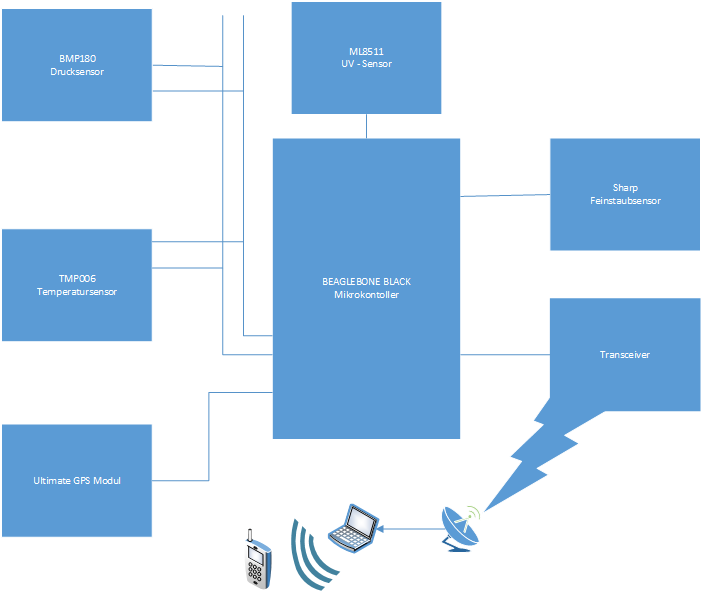
\includegraphics[width=0.8\textwidth]{8_Anhang/Blockdiagramm.png}
	\caption{Blockdiagramm vom CANSAT}
	\label{blockdiagramm}
\end{figure}

\newpage

\subsection{GANTT-Diagramme}
\subsubsection {Hardware-GANTT}
\begin{figure}[htbp]
	\centering
	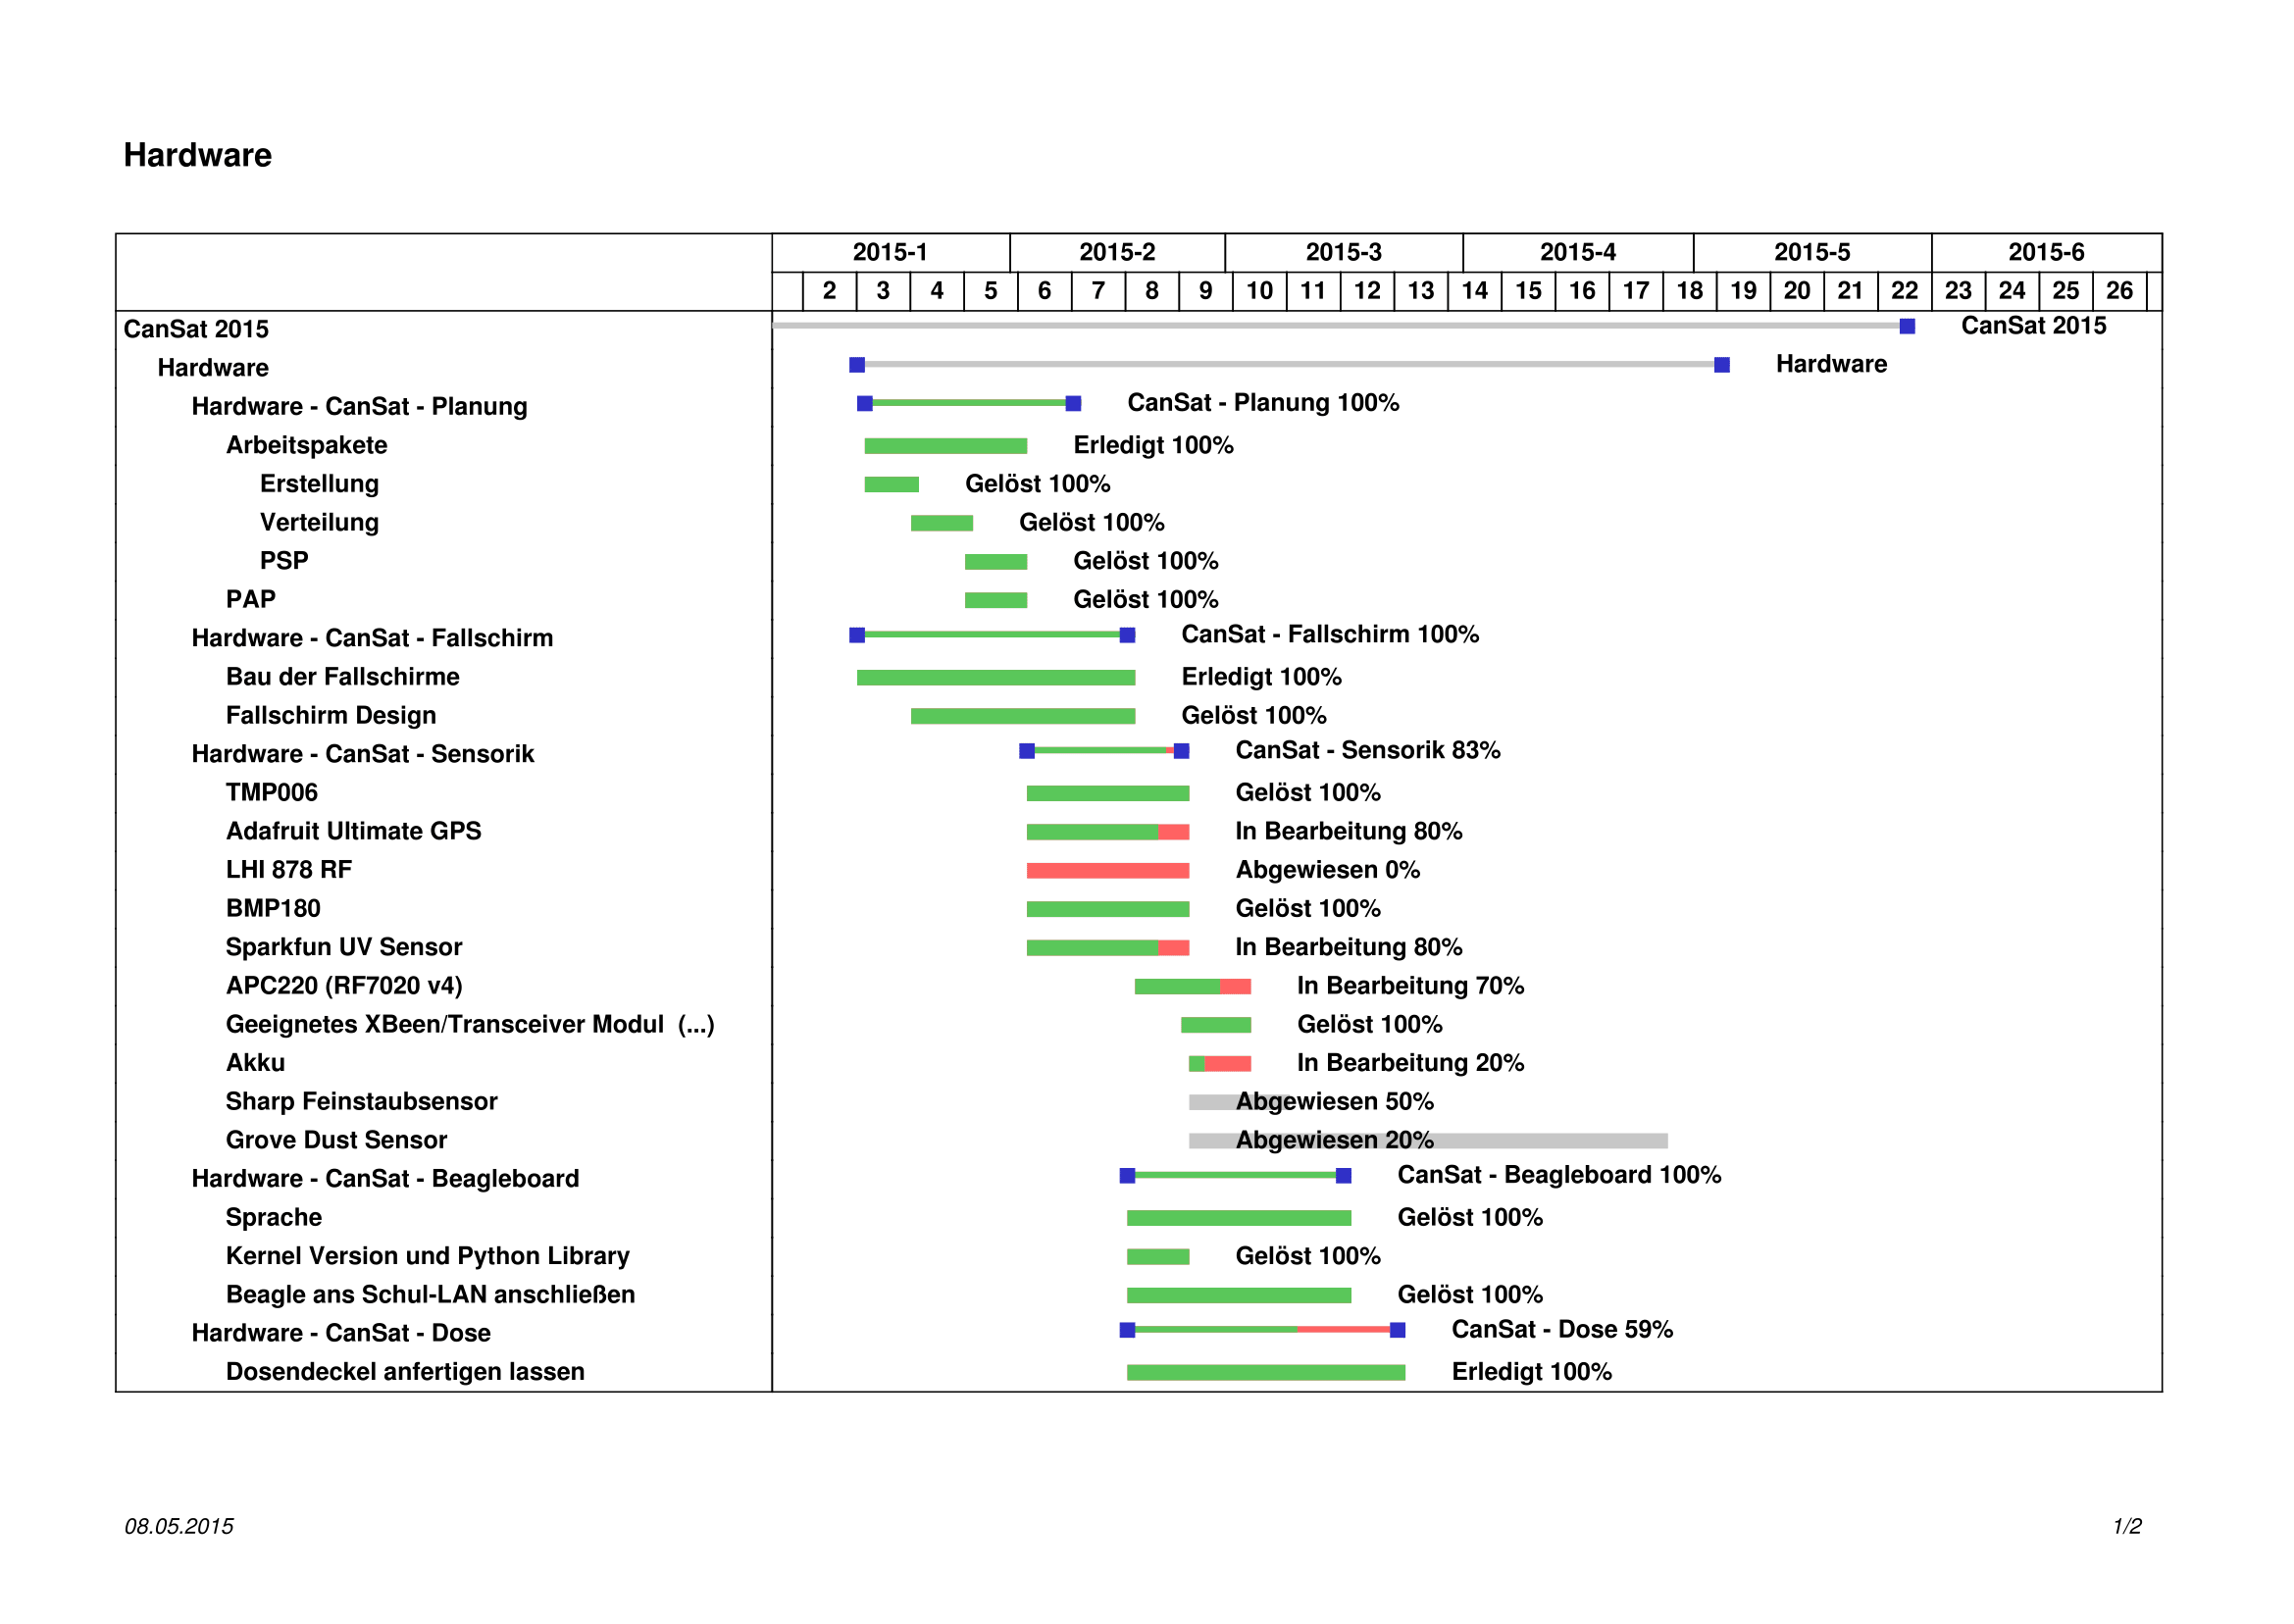
\includegraphics[trim = 10mm 50mm 20mm 65mm, clip,width=0.8\textwidth]{8_Anhang/hardware-gantt-1.png}
	\label{gantt_hardware_1}
\end{figure}
\vspace{-2cm}
\begin{figure}[htbp]
	\centering
	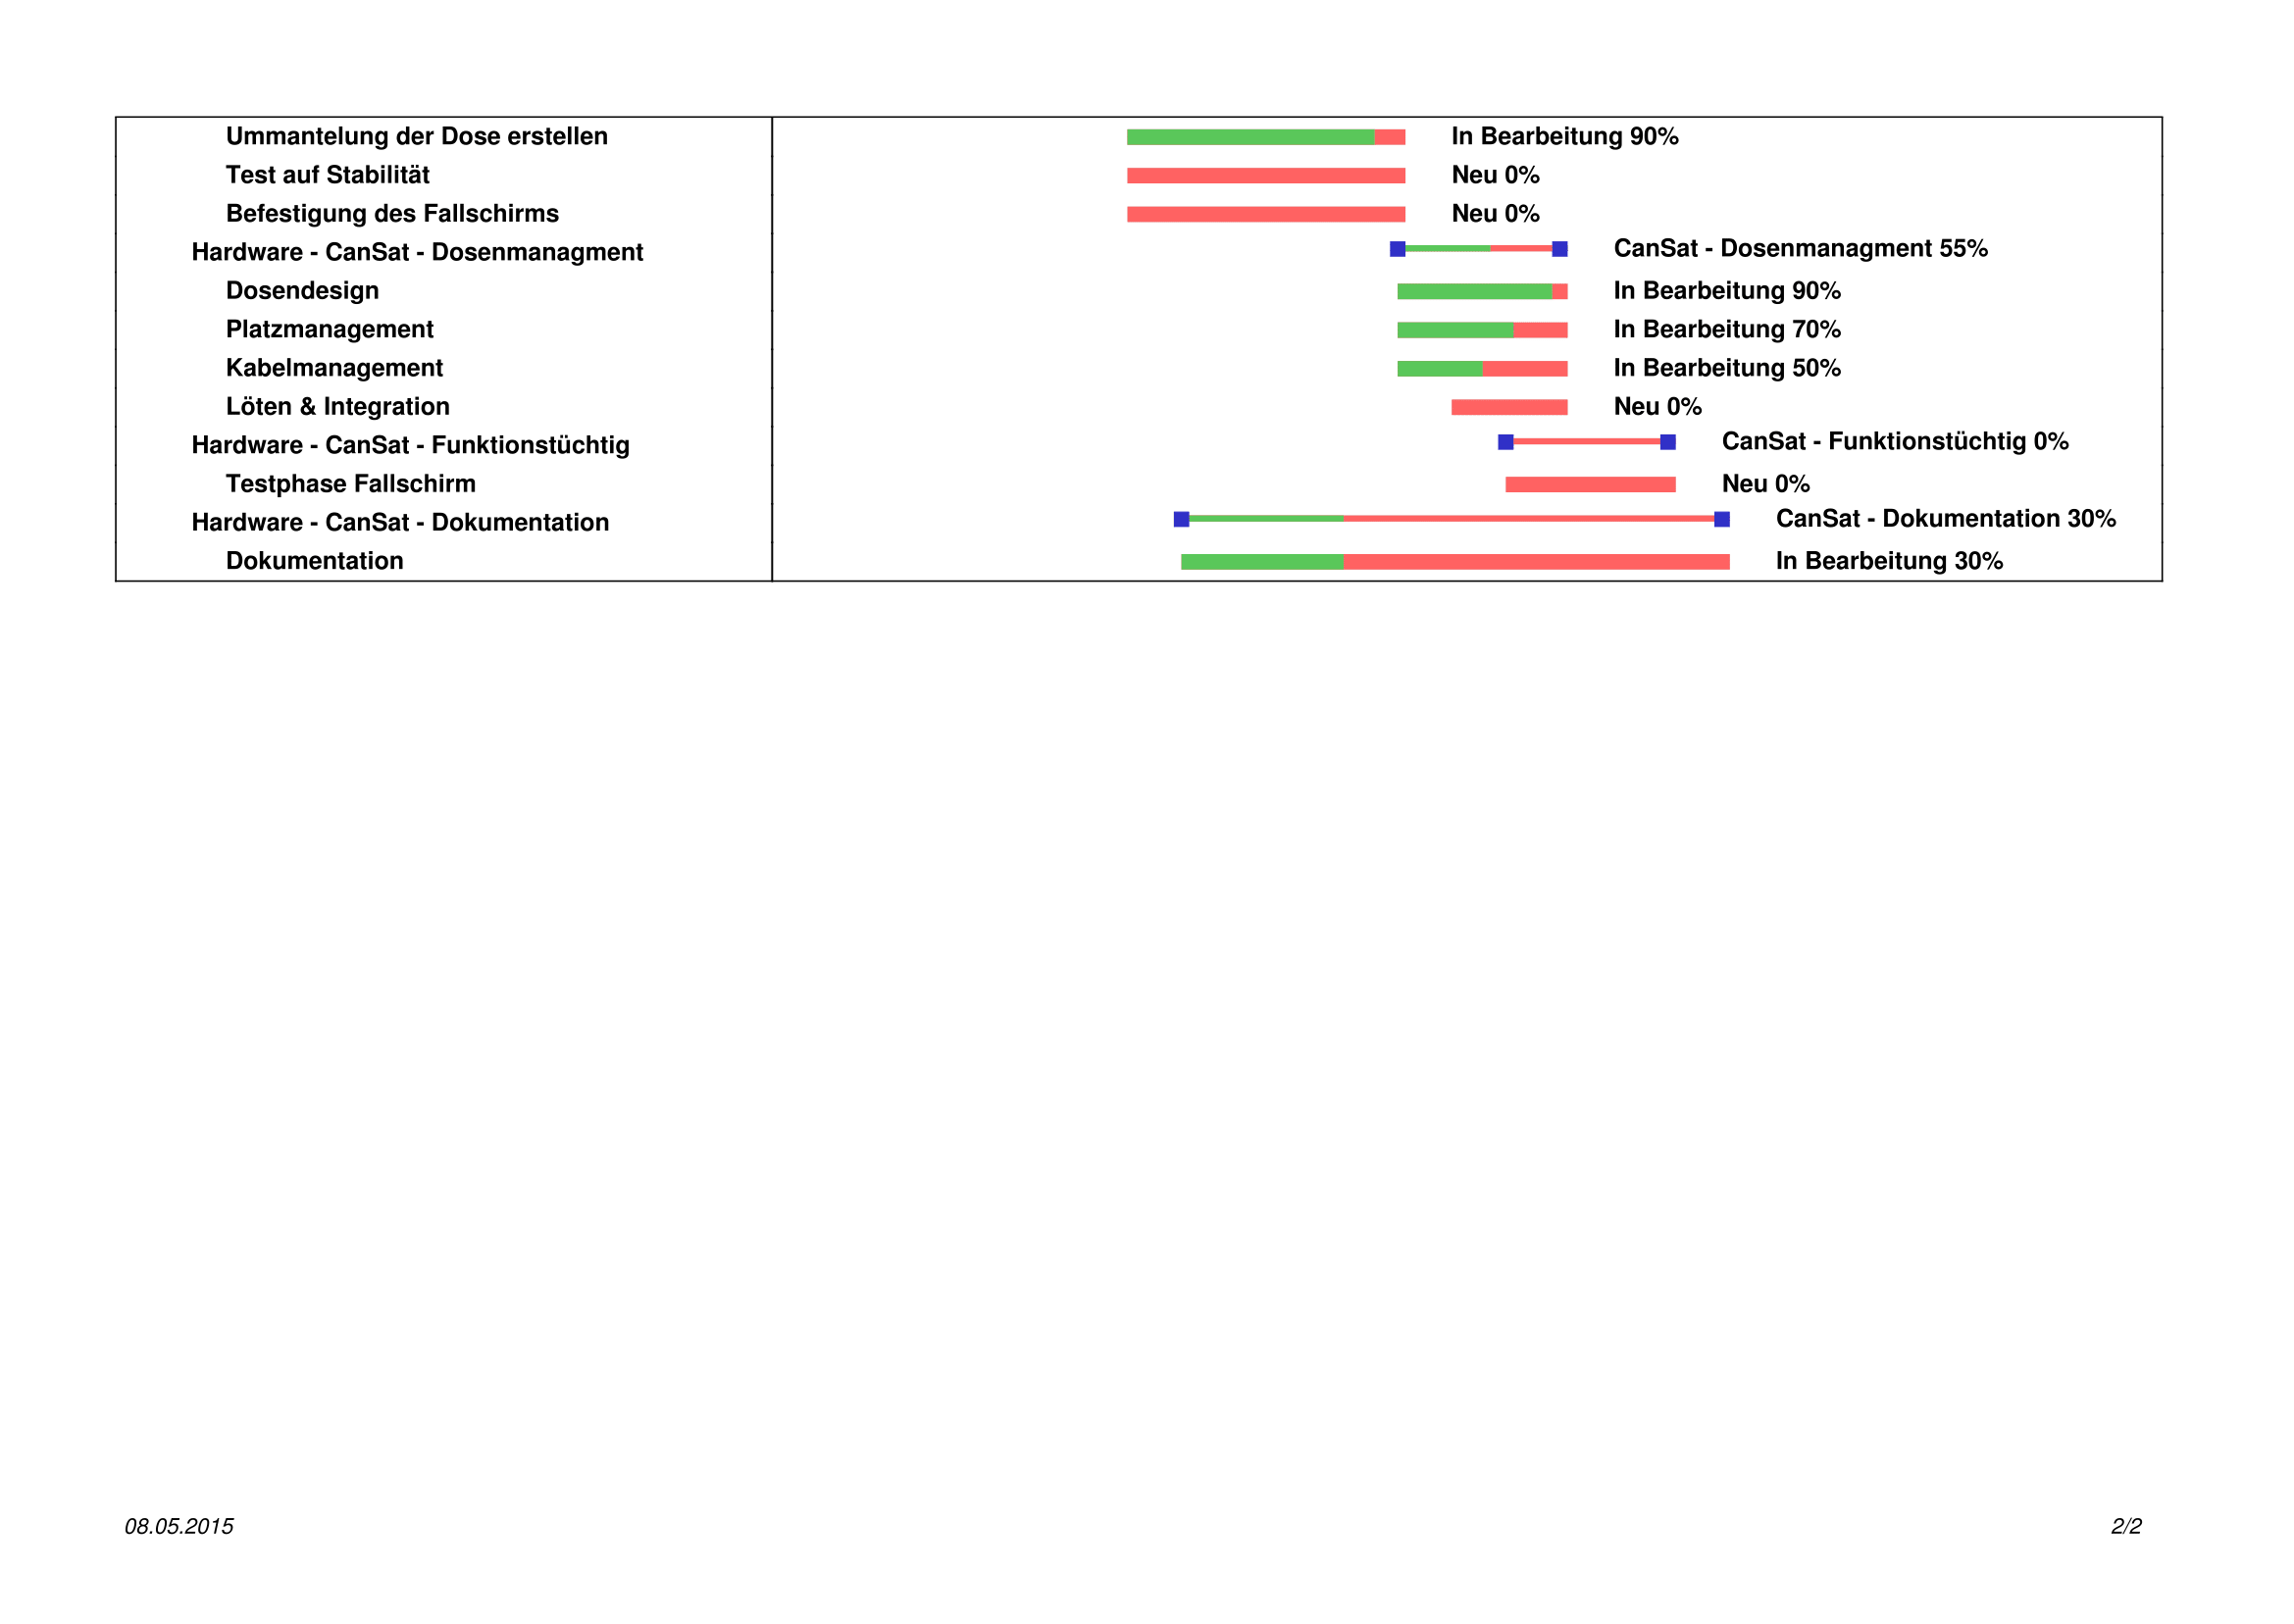
\includegraphics[trim = 11mm 350mm 20mm 40mm, clip,width=0.8\textwidth]{8_Anhang/hardware-gantt-2.png}
	\caption{Das GANTT-Diagramm der Hardware Gruppe}
	\label{gantt_hardware_2}
\end{figure}

\newpage
\subsubsection {Bodenstation-GANTT}
\begin{figure}[H]
	\centering
	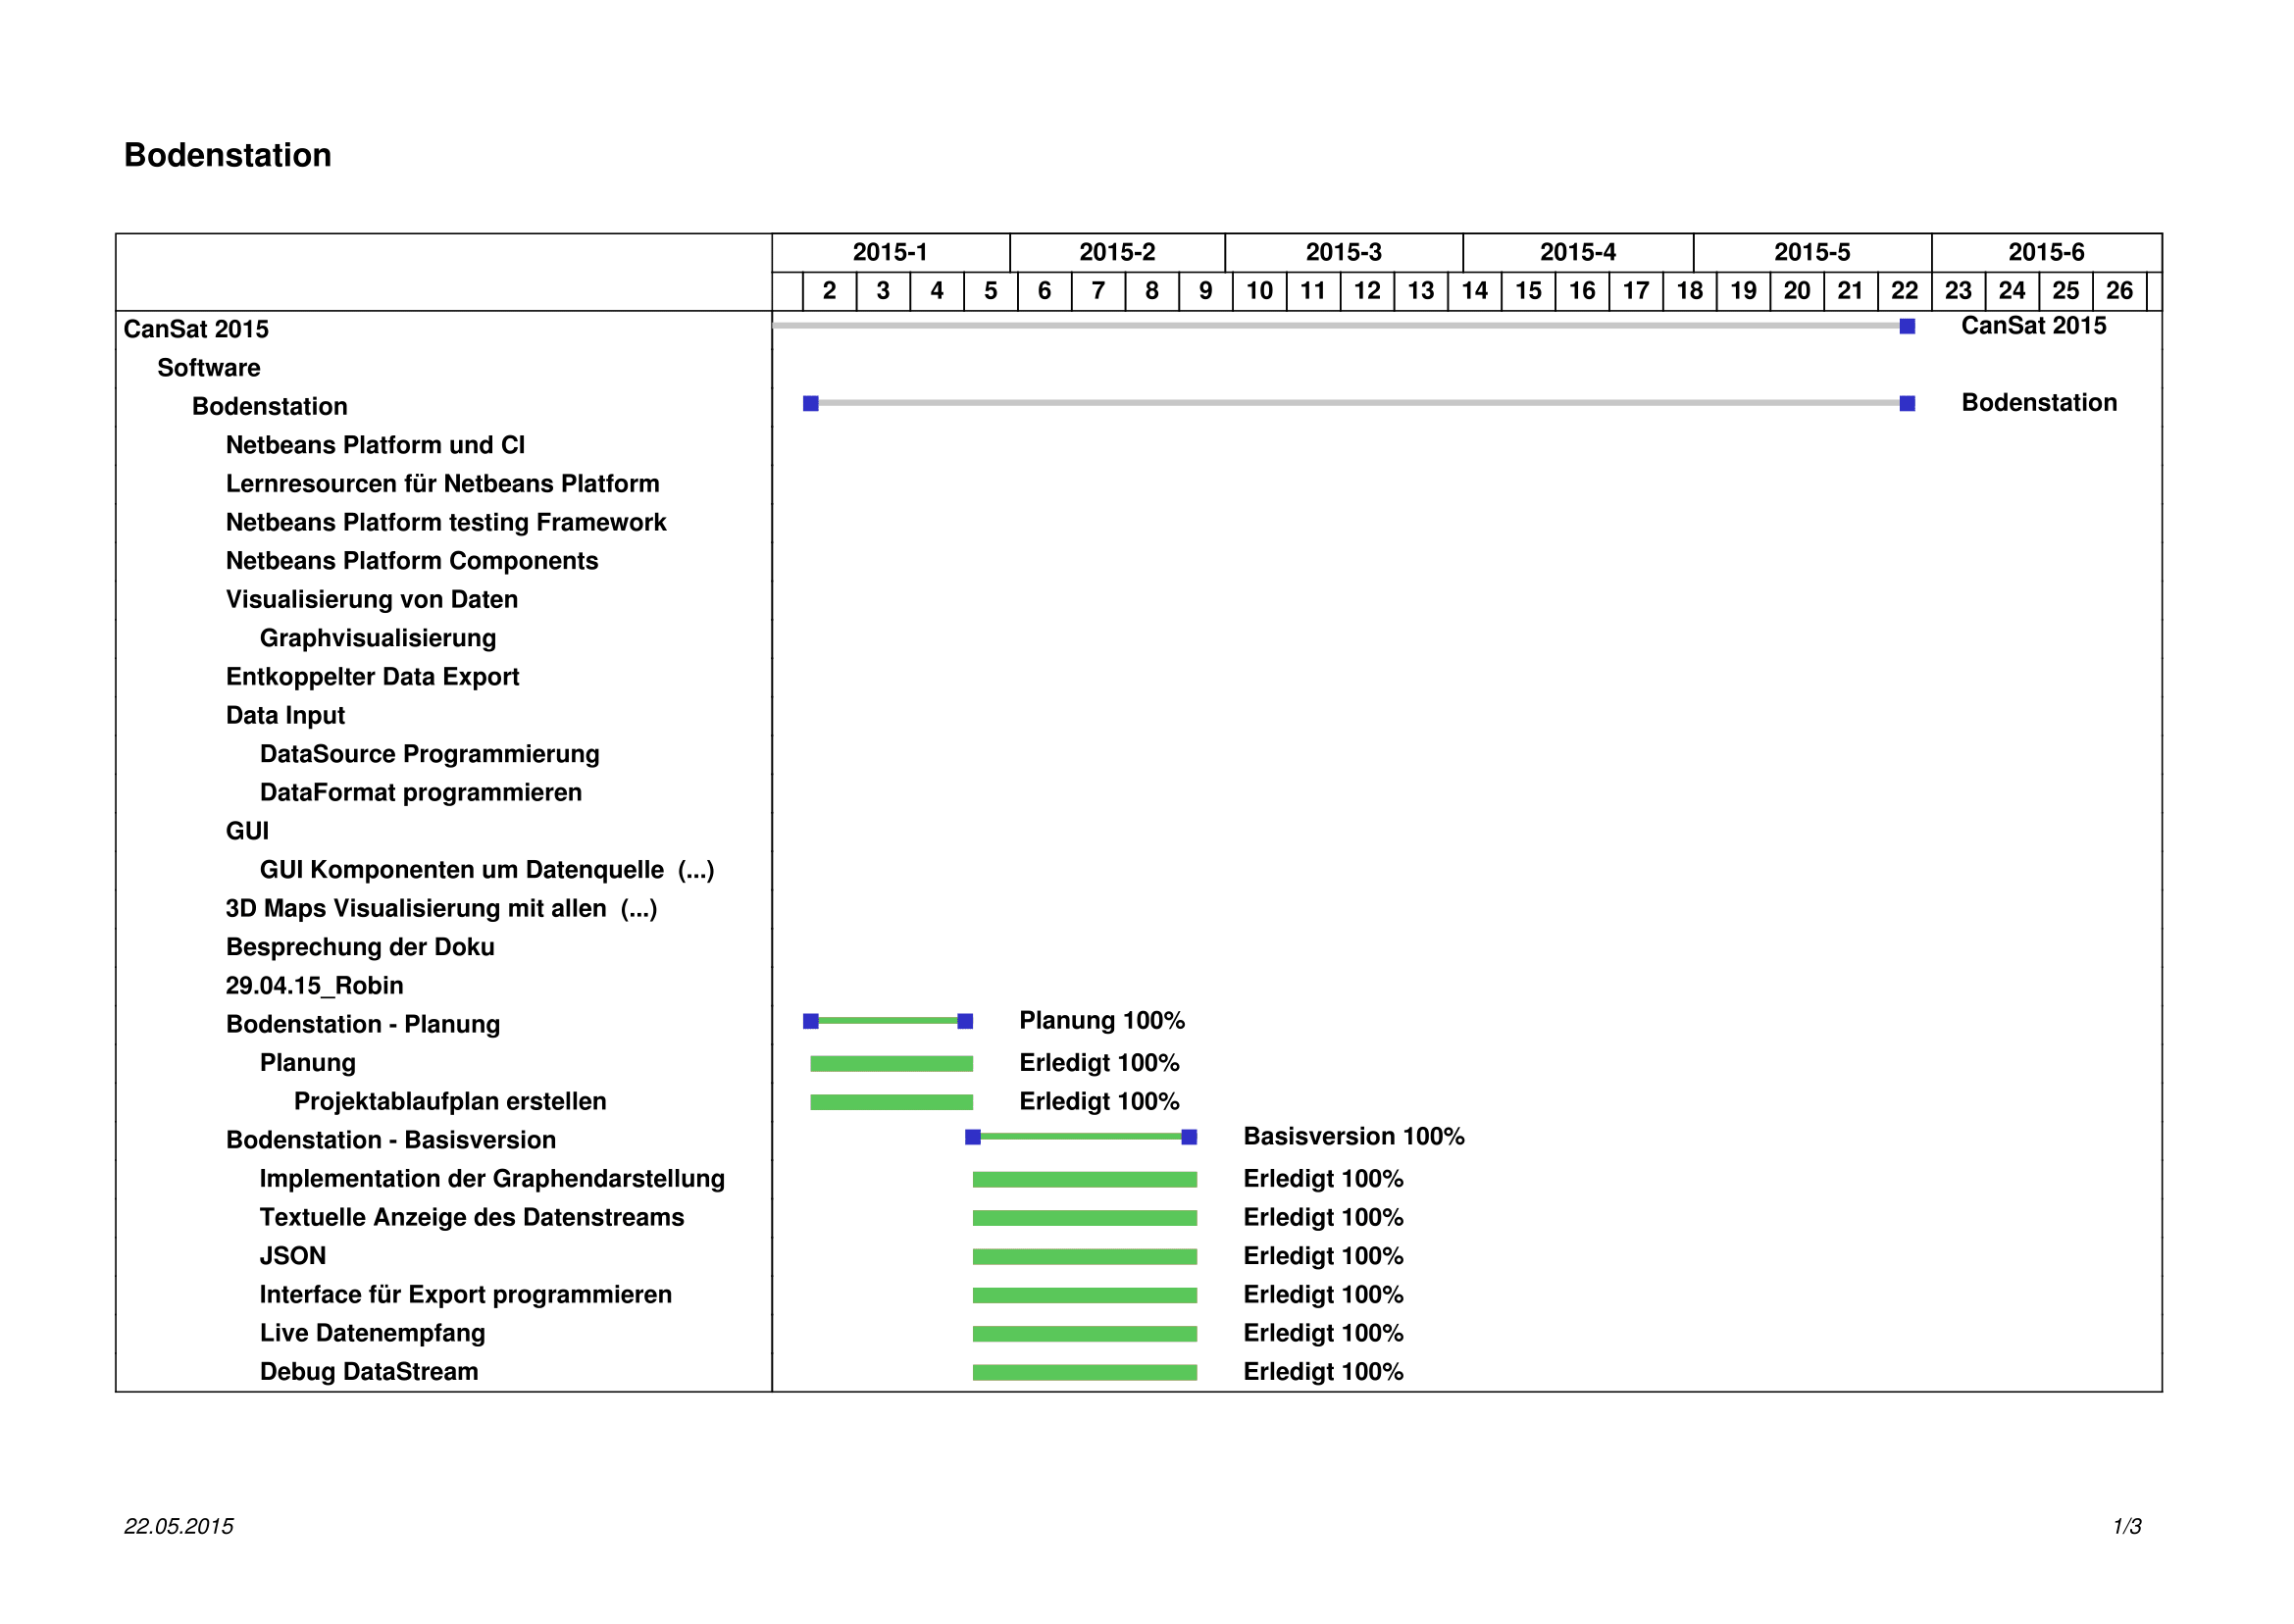
\includegraphics[trim = 25mm 50mm 46mm 65mm, clip,width=0.8\textwidth]{8_Anhang/bodenstation-gantt-1.png}
	\label{gantt_hardware_1}
\end{figure}
\vspace{-1,3cm}
\begin{figure}[H]
	\centering
	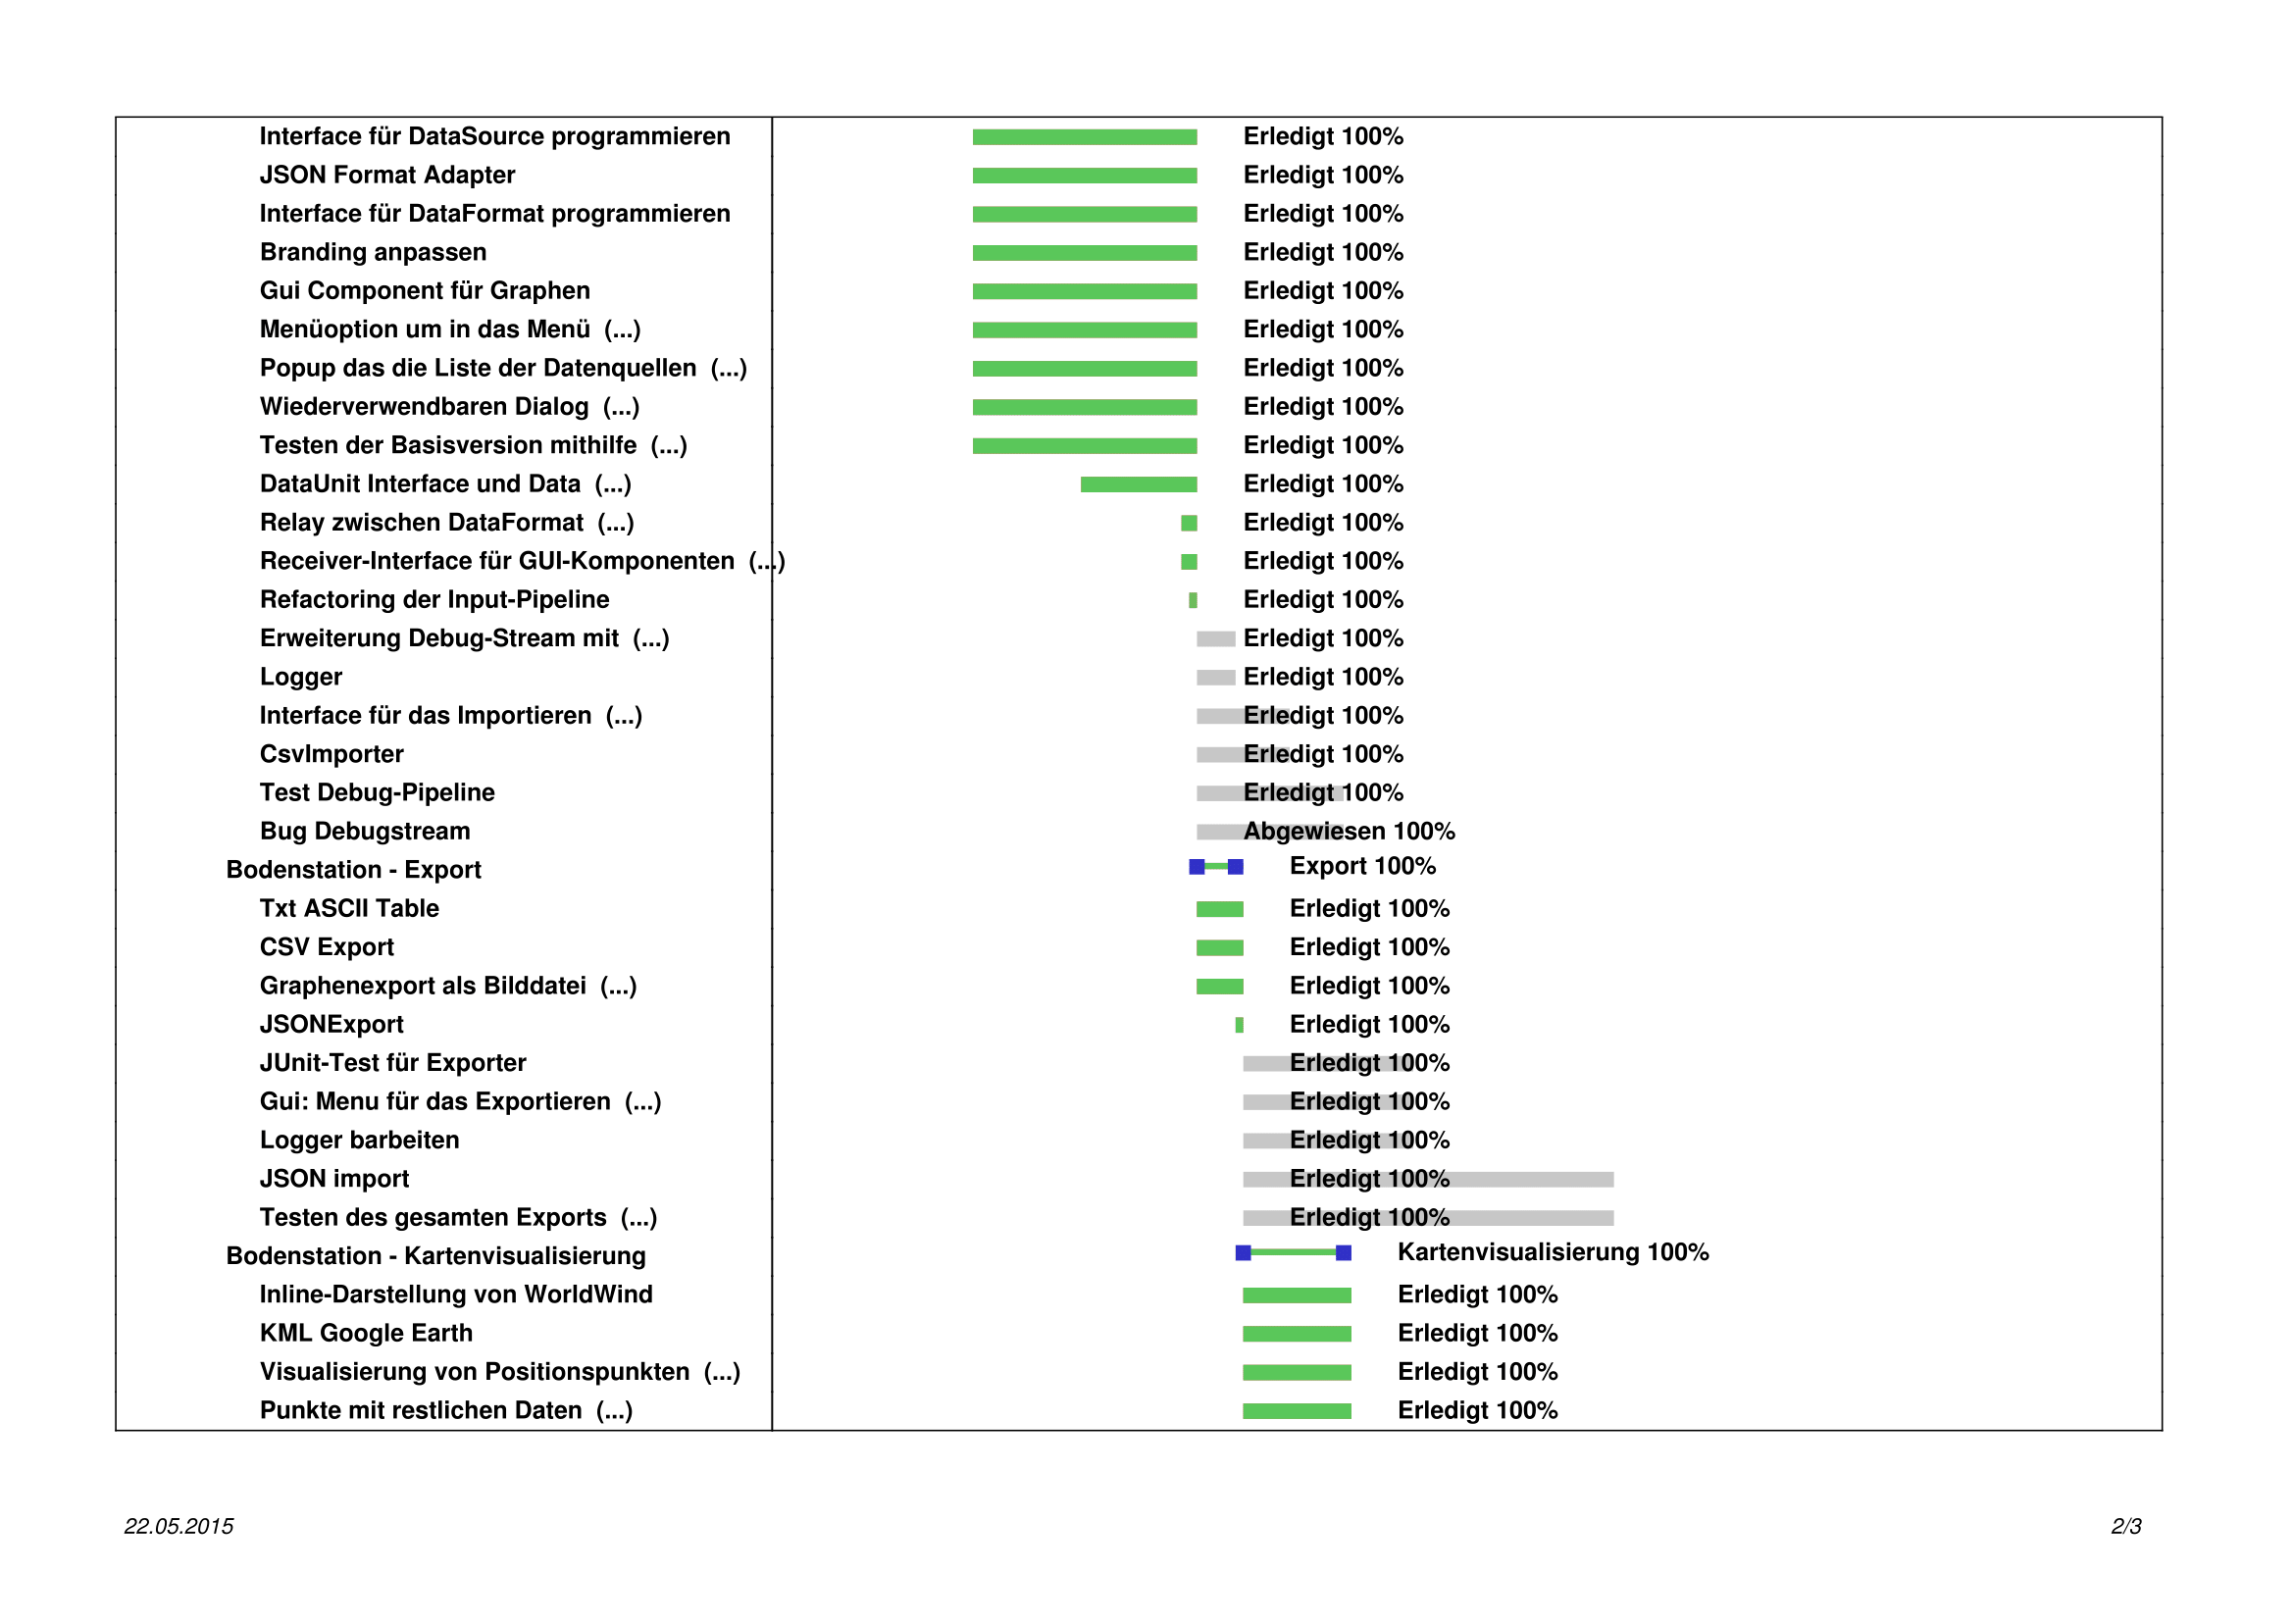
\includegraphics[trim = 30mm 50mm 45mm 40mm, clip,width=0.8\textwidth]{8_Anhang/bodenstation-gantt-2.png}
	\label{gantt_hardware_2}
\end{figure}
\vspace{-1,1cm}
\begin{figure}[H]
	\centering
	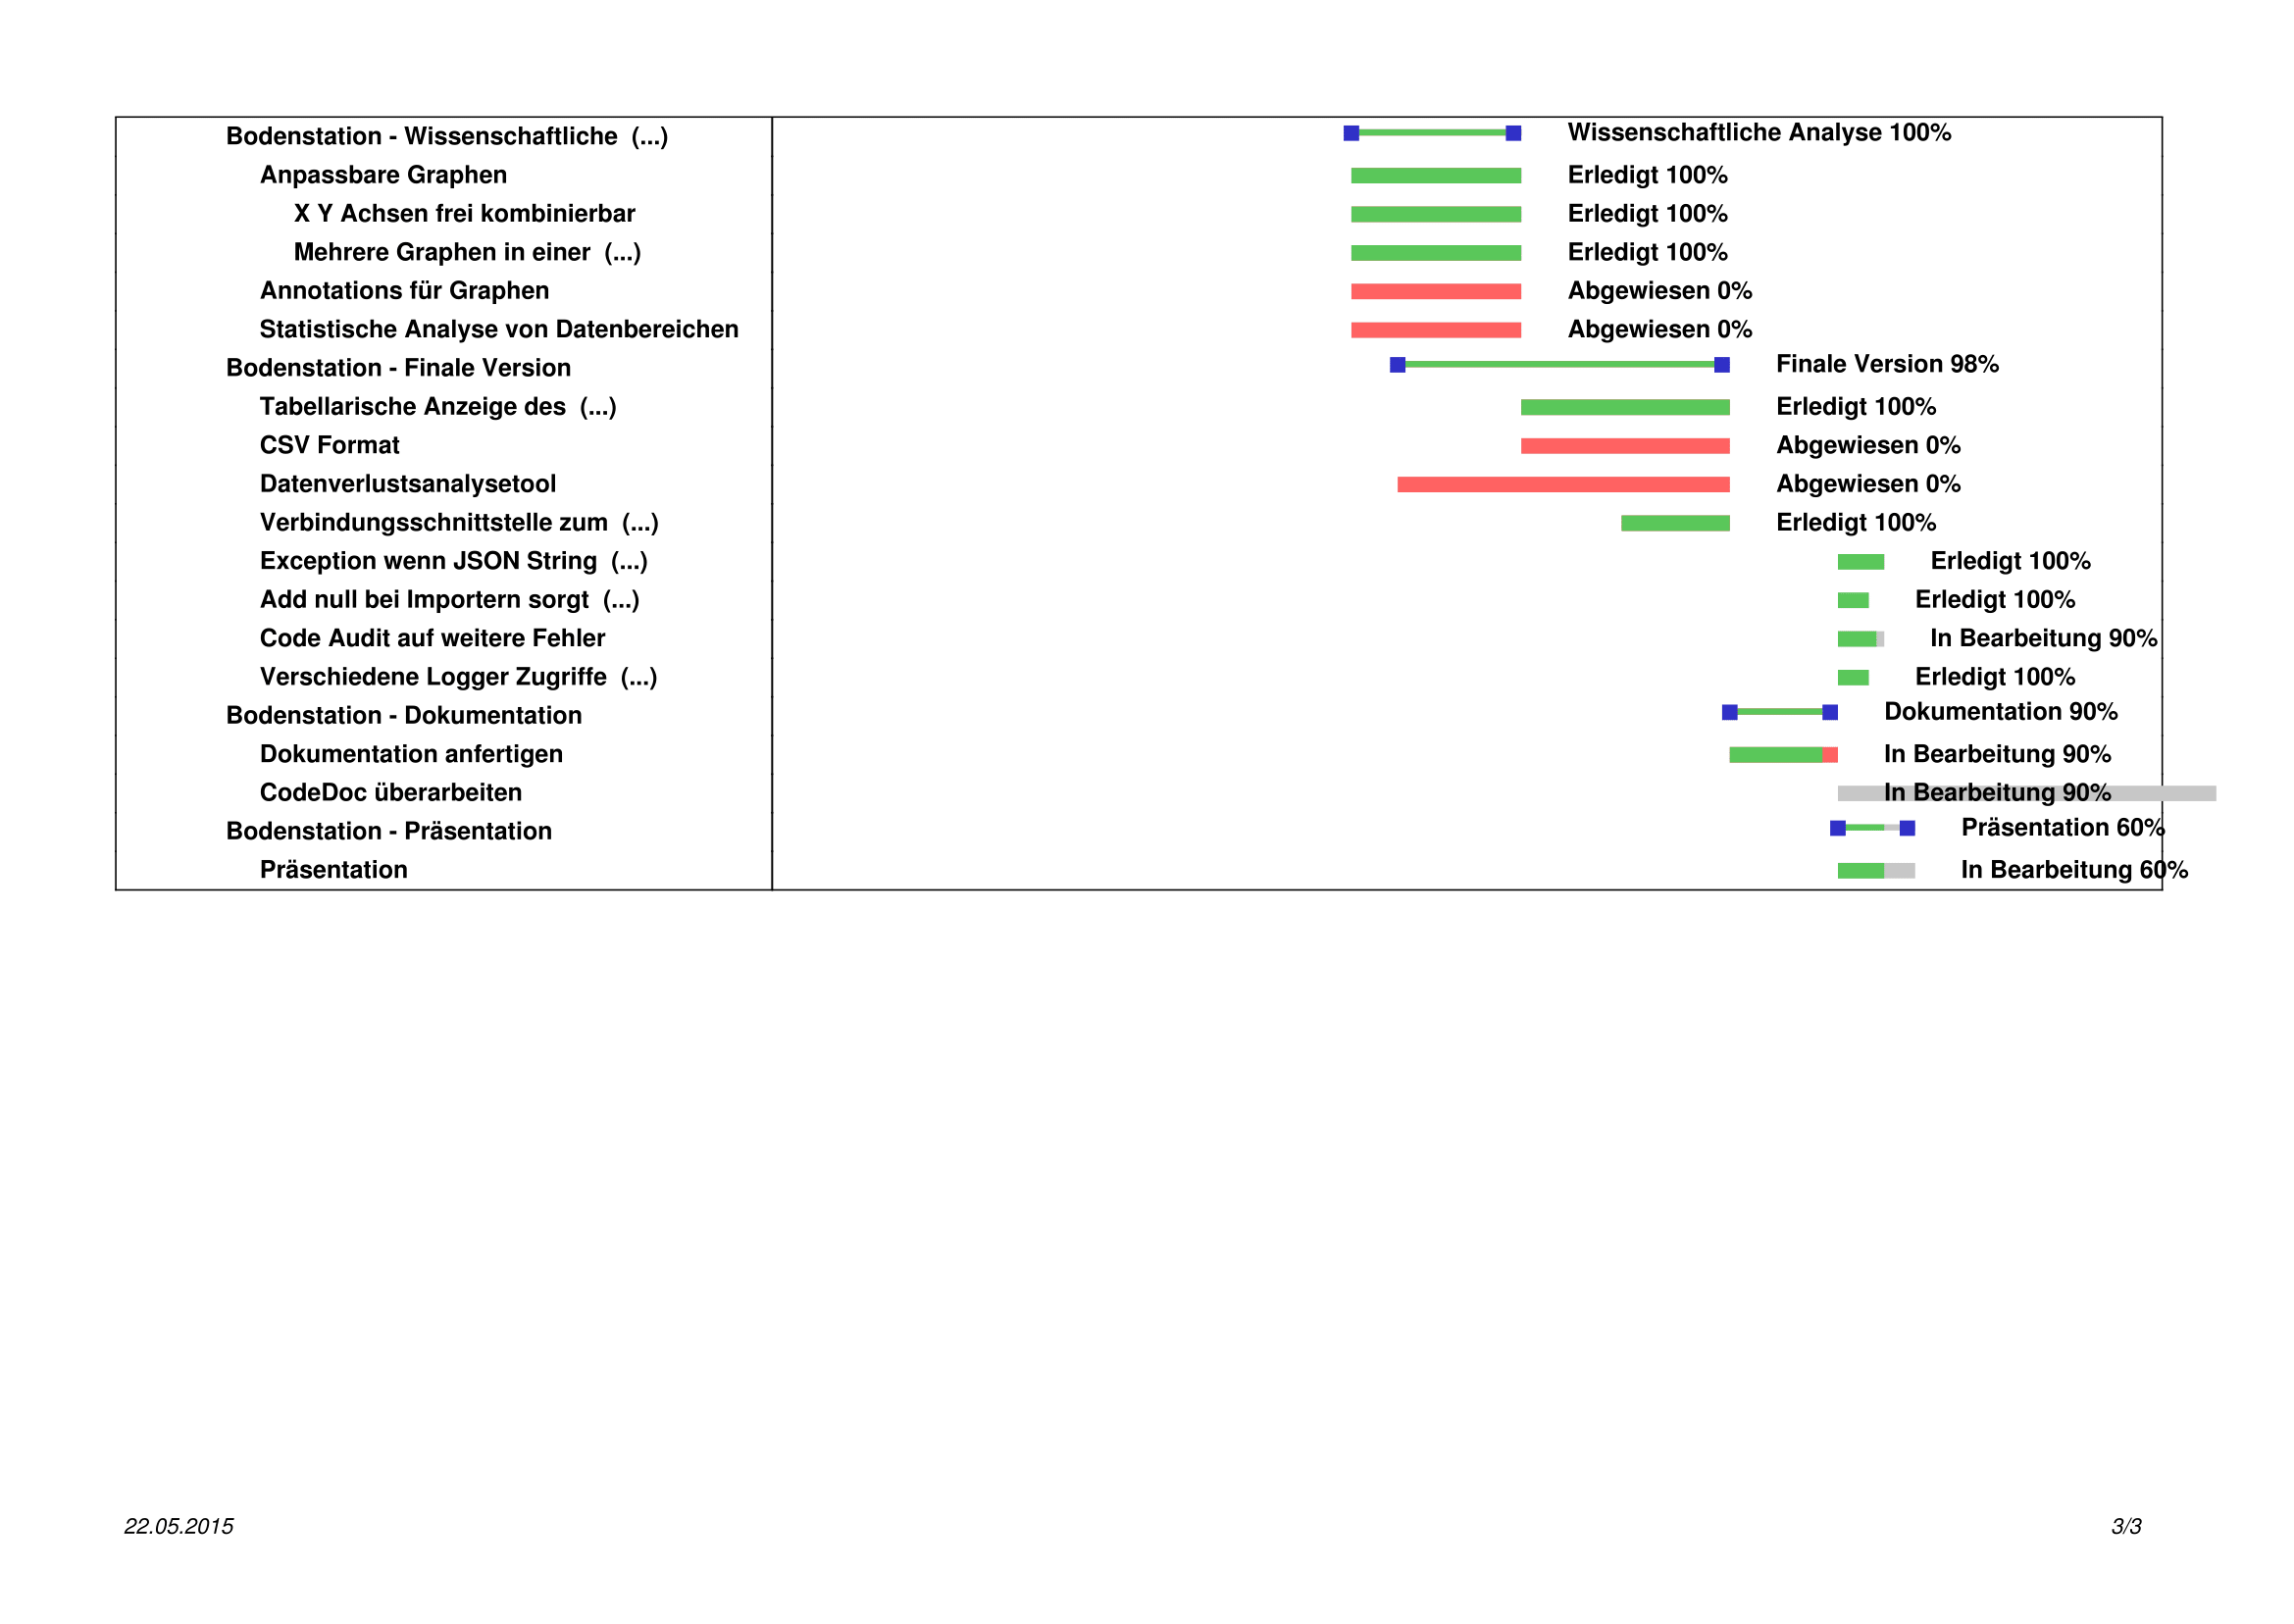
\includegraphics[trim = 30mm 200mm 45mm 40mm, clip,width=0.8\textwidth]{8_Anhang/bodenstation-gantt-3.png}
	\caption{Das GANTT-Diagramm der Bodenstation}
	\label{gantt_hardware_3}
\end{figure}
\newpage
\subsubsection {Android-App-GANTT}
\begin{figure}[H]
	\centering
	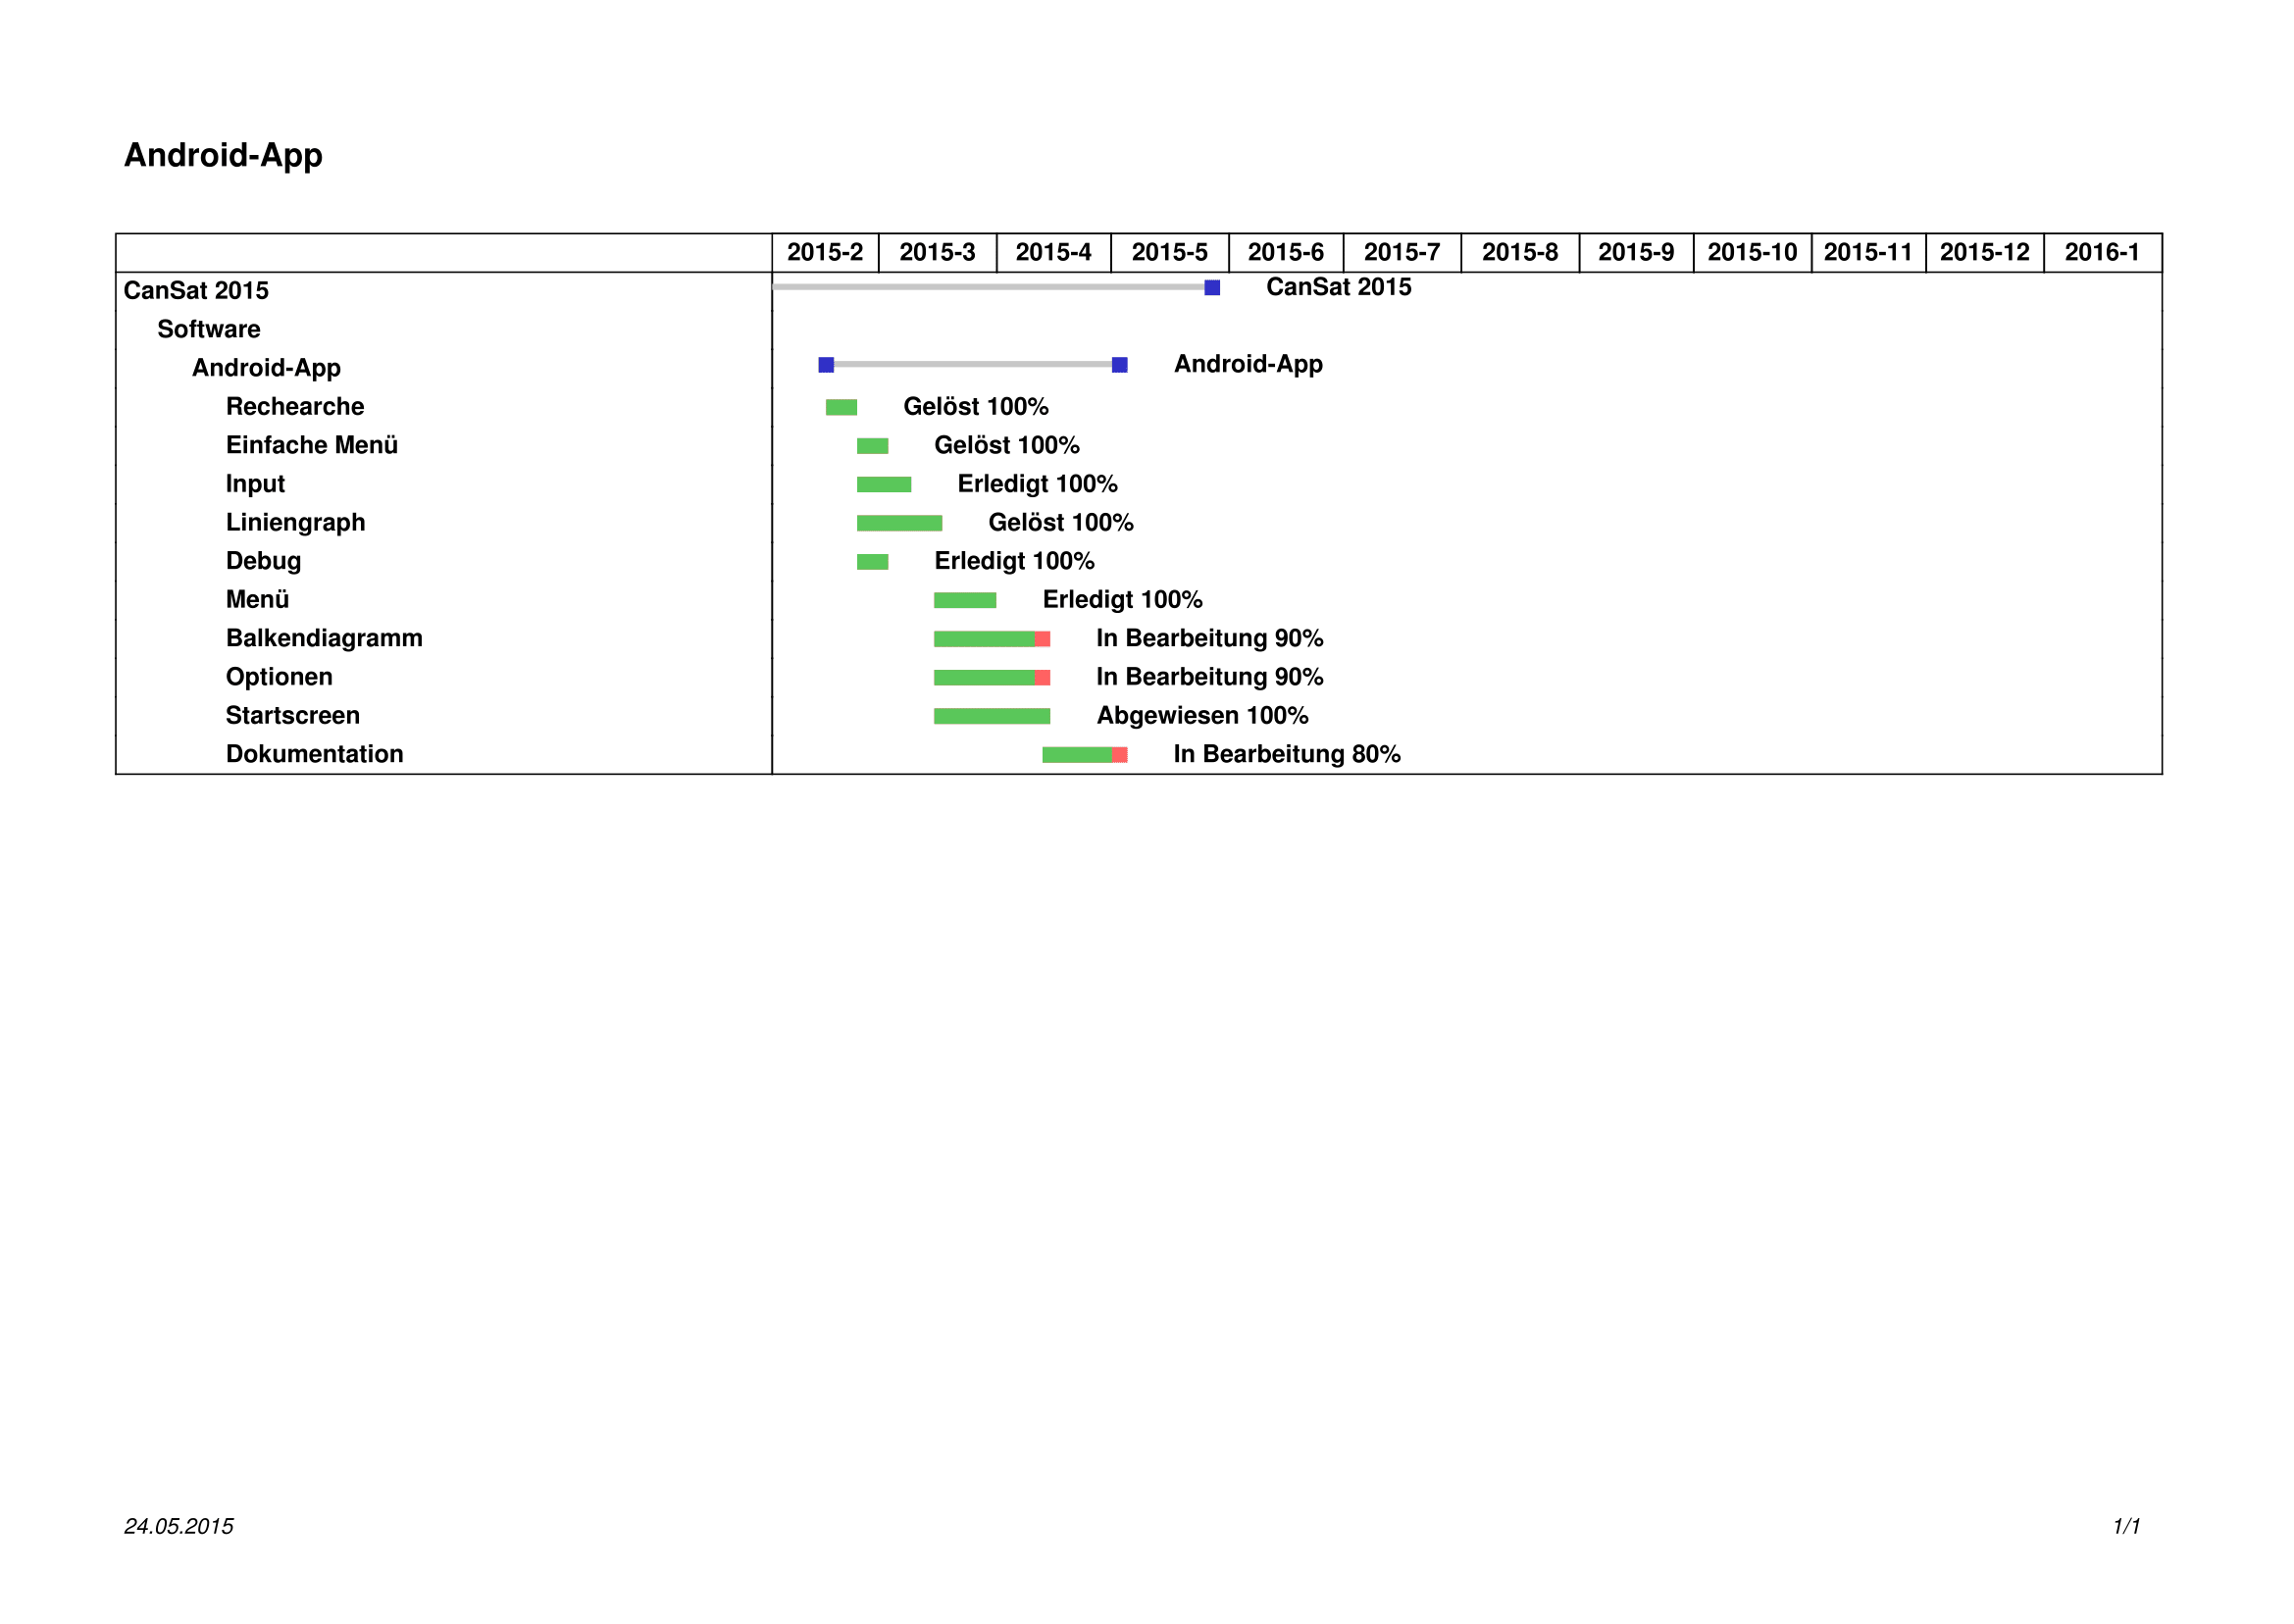
\includegraphics[trim = 30mm 200mm 45mm 40mm, clip,width=0.8\textwidth]{8_Anhang/android-app-gantt.png}
	\caption{Das GANTT-Diagramm der Android App}
	\label{gantt_hardware_3}
\end{figure}

\newpage
\vspace{-2cm}
\subsection{Der CanSat}

\begin{figure}[H]
	\centering
	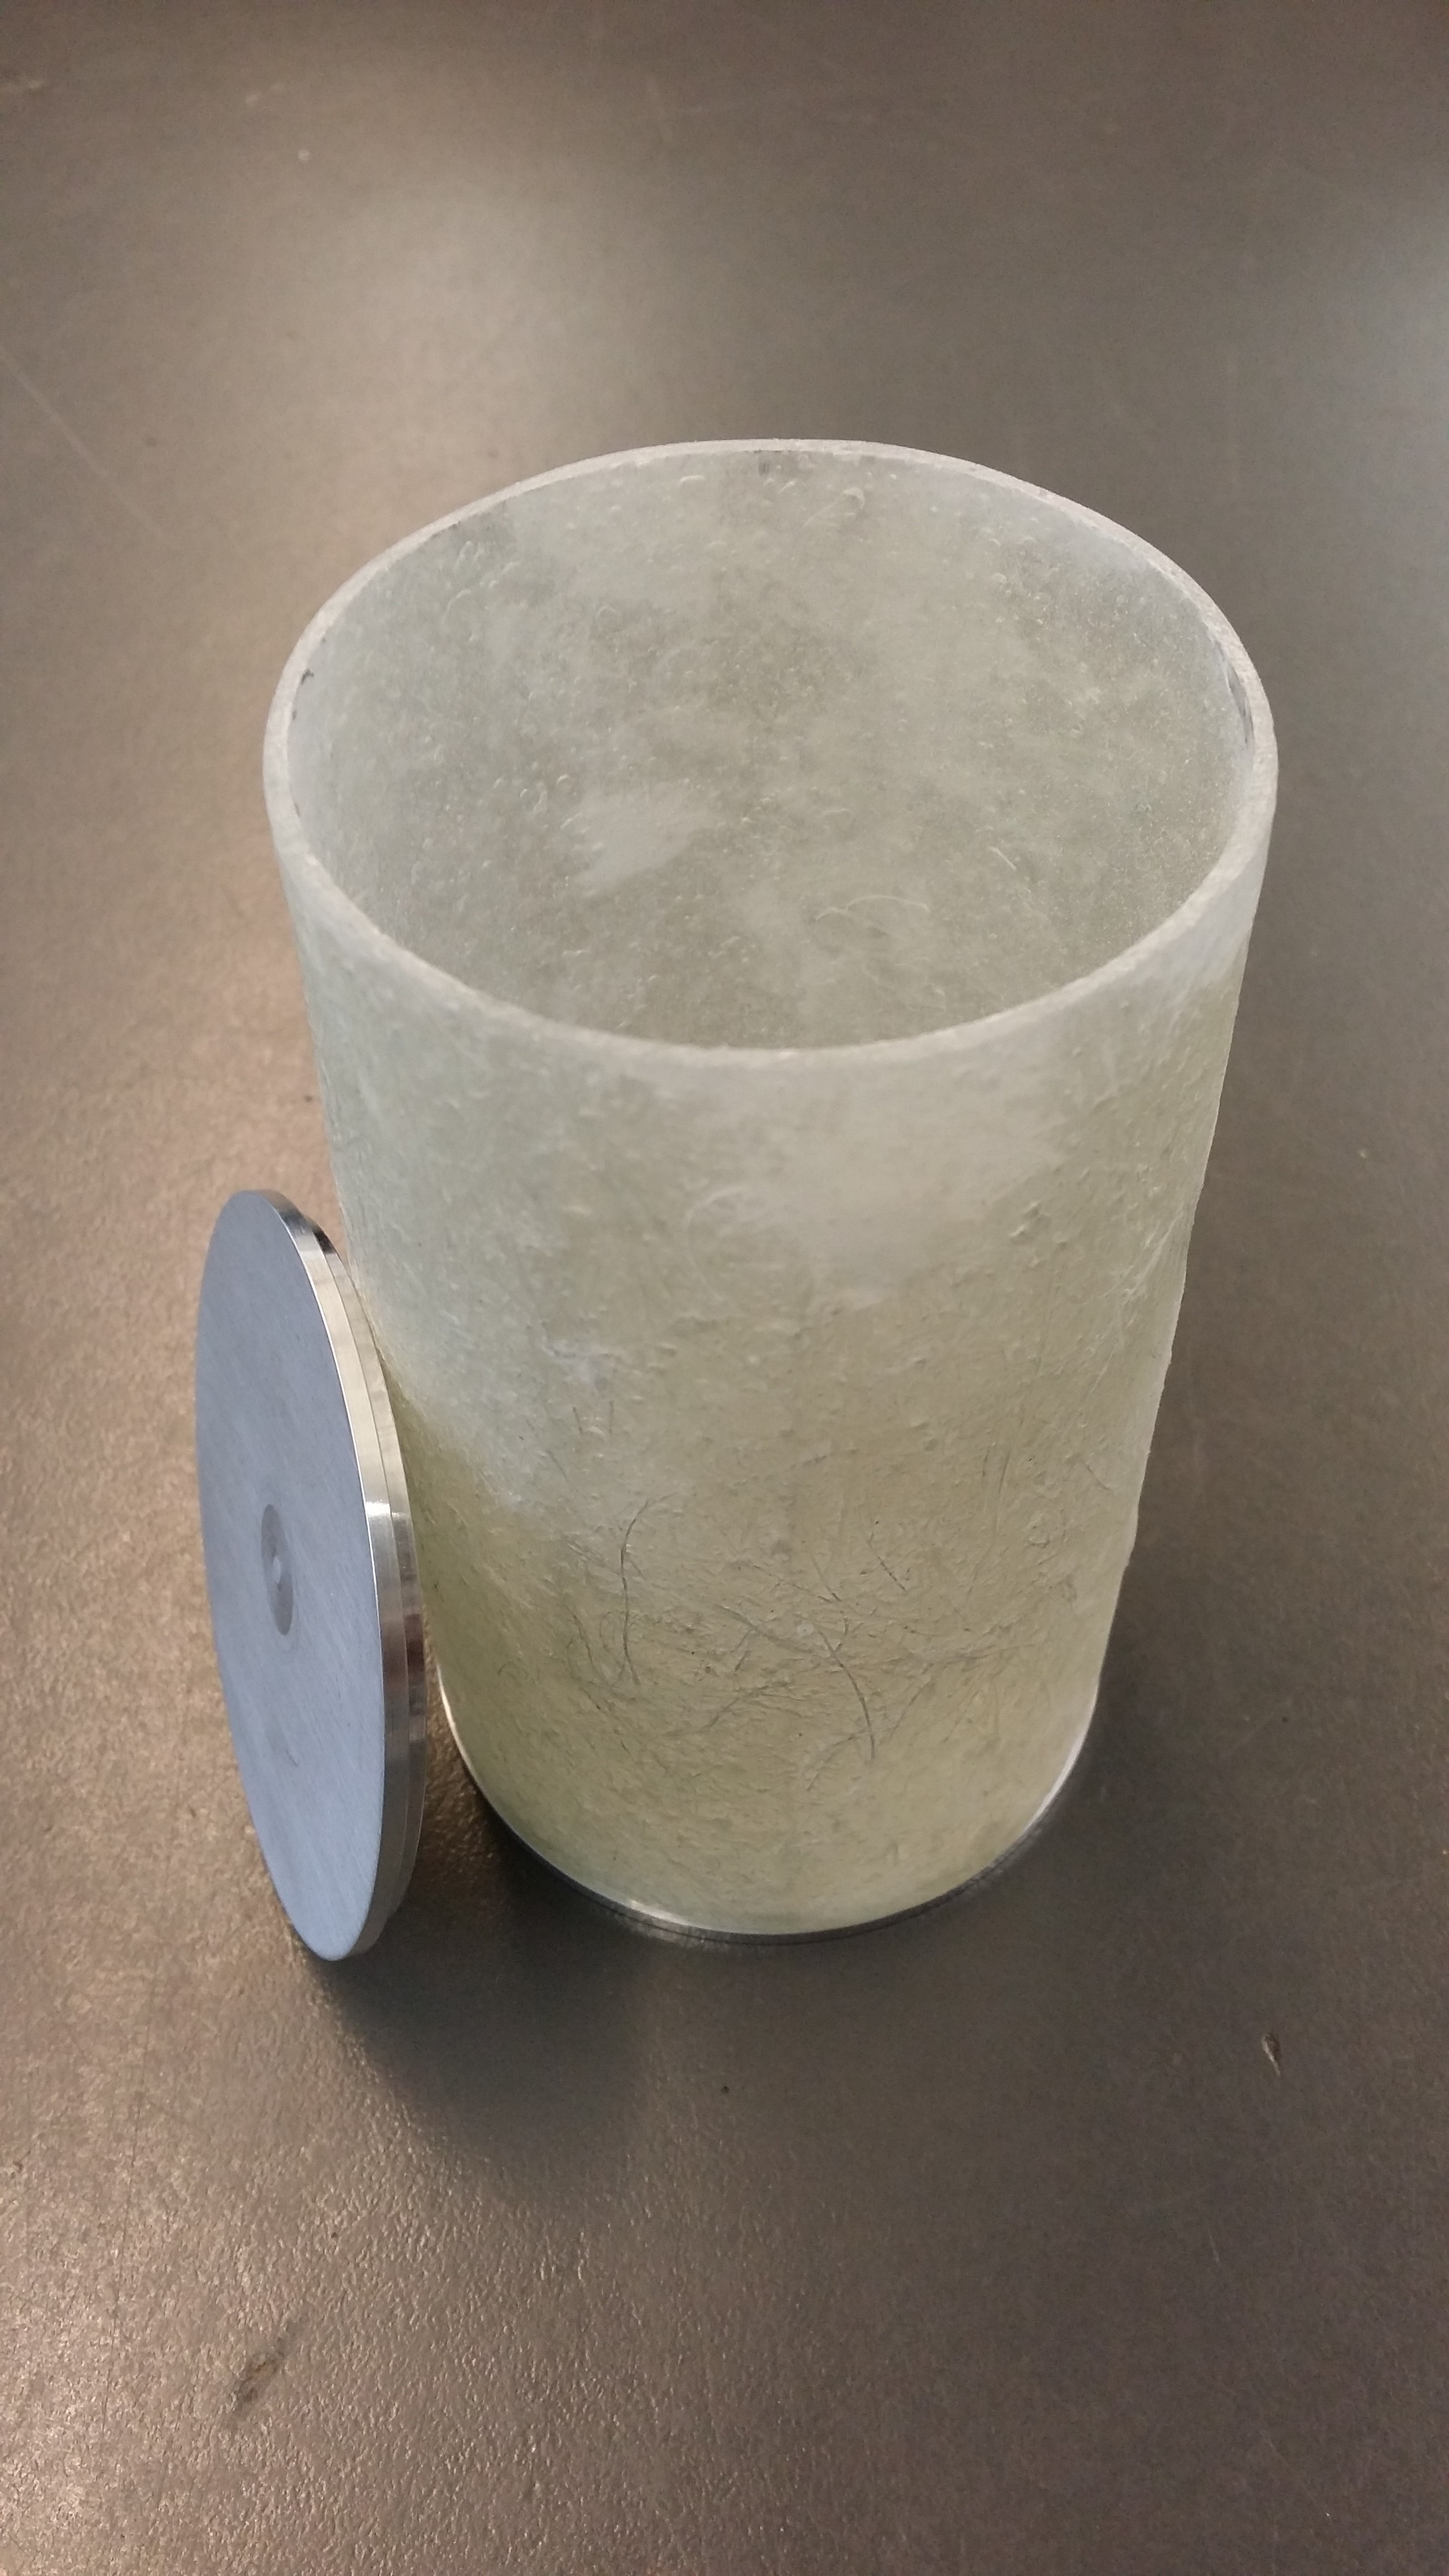
\includegraphics[trim = 11mm 335mm 20mm 210mm, clip, width=0.8\textwidth]{8_Anhang/dose.jpg}
	\caption{Die Hülle und ein Dosendeckel}
	\label{pic_dose}
\end{figure}

\begin{figure}[H]
	\centering
	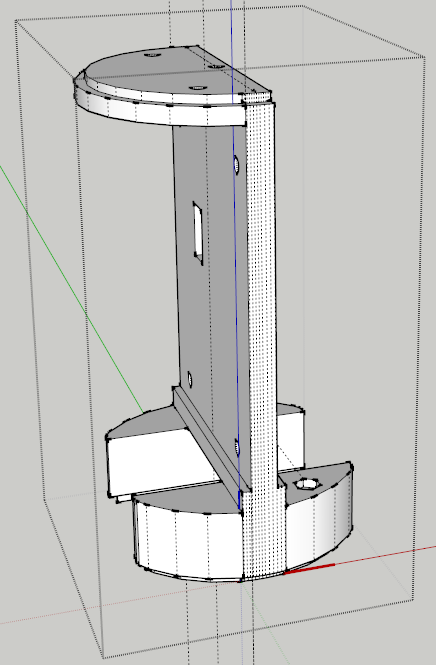
\includegraphics[ width=0.8\textwidth]{8_Anhang/Wand_3D.PNG}
	\caption{Screenshot der Zwischenwand aus Sketchup}
	\label{pic_wand_3d}
\end{figure}

\newpage

\begin{figure}[h] 
      \centering 
      \includemovie[ 
        poster,controls,
       3Djscript=2_Beschreibung_des_CANSAT/Encompass.js
      ]{0.8\textwidth}{15cm}{2_Beschreibung_des_CANSAT/CanSat_2015.u3d} 
      \caption{Der Satellit (Diese Zeichnung ist möglicherweiße nicht sichtbar, da es eine 3D Zeichnung ist. Bitte verwenden Sie den \href{https://get.adobe.com/reader/?loc=de}{Adobe Acrobat Reader})}\label{pic_3d} 
\end{figure} 

\newpage

\begin{figure}[H]
	\centering
	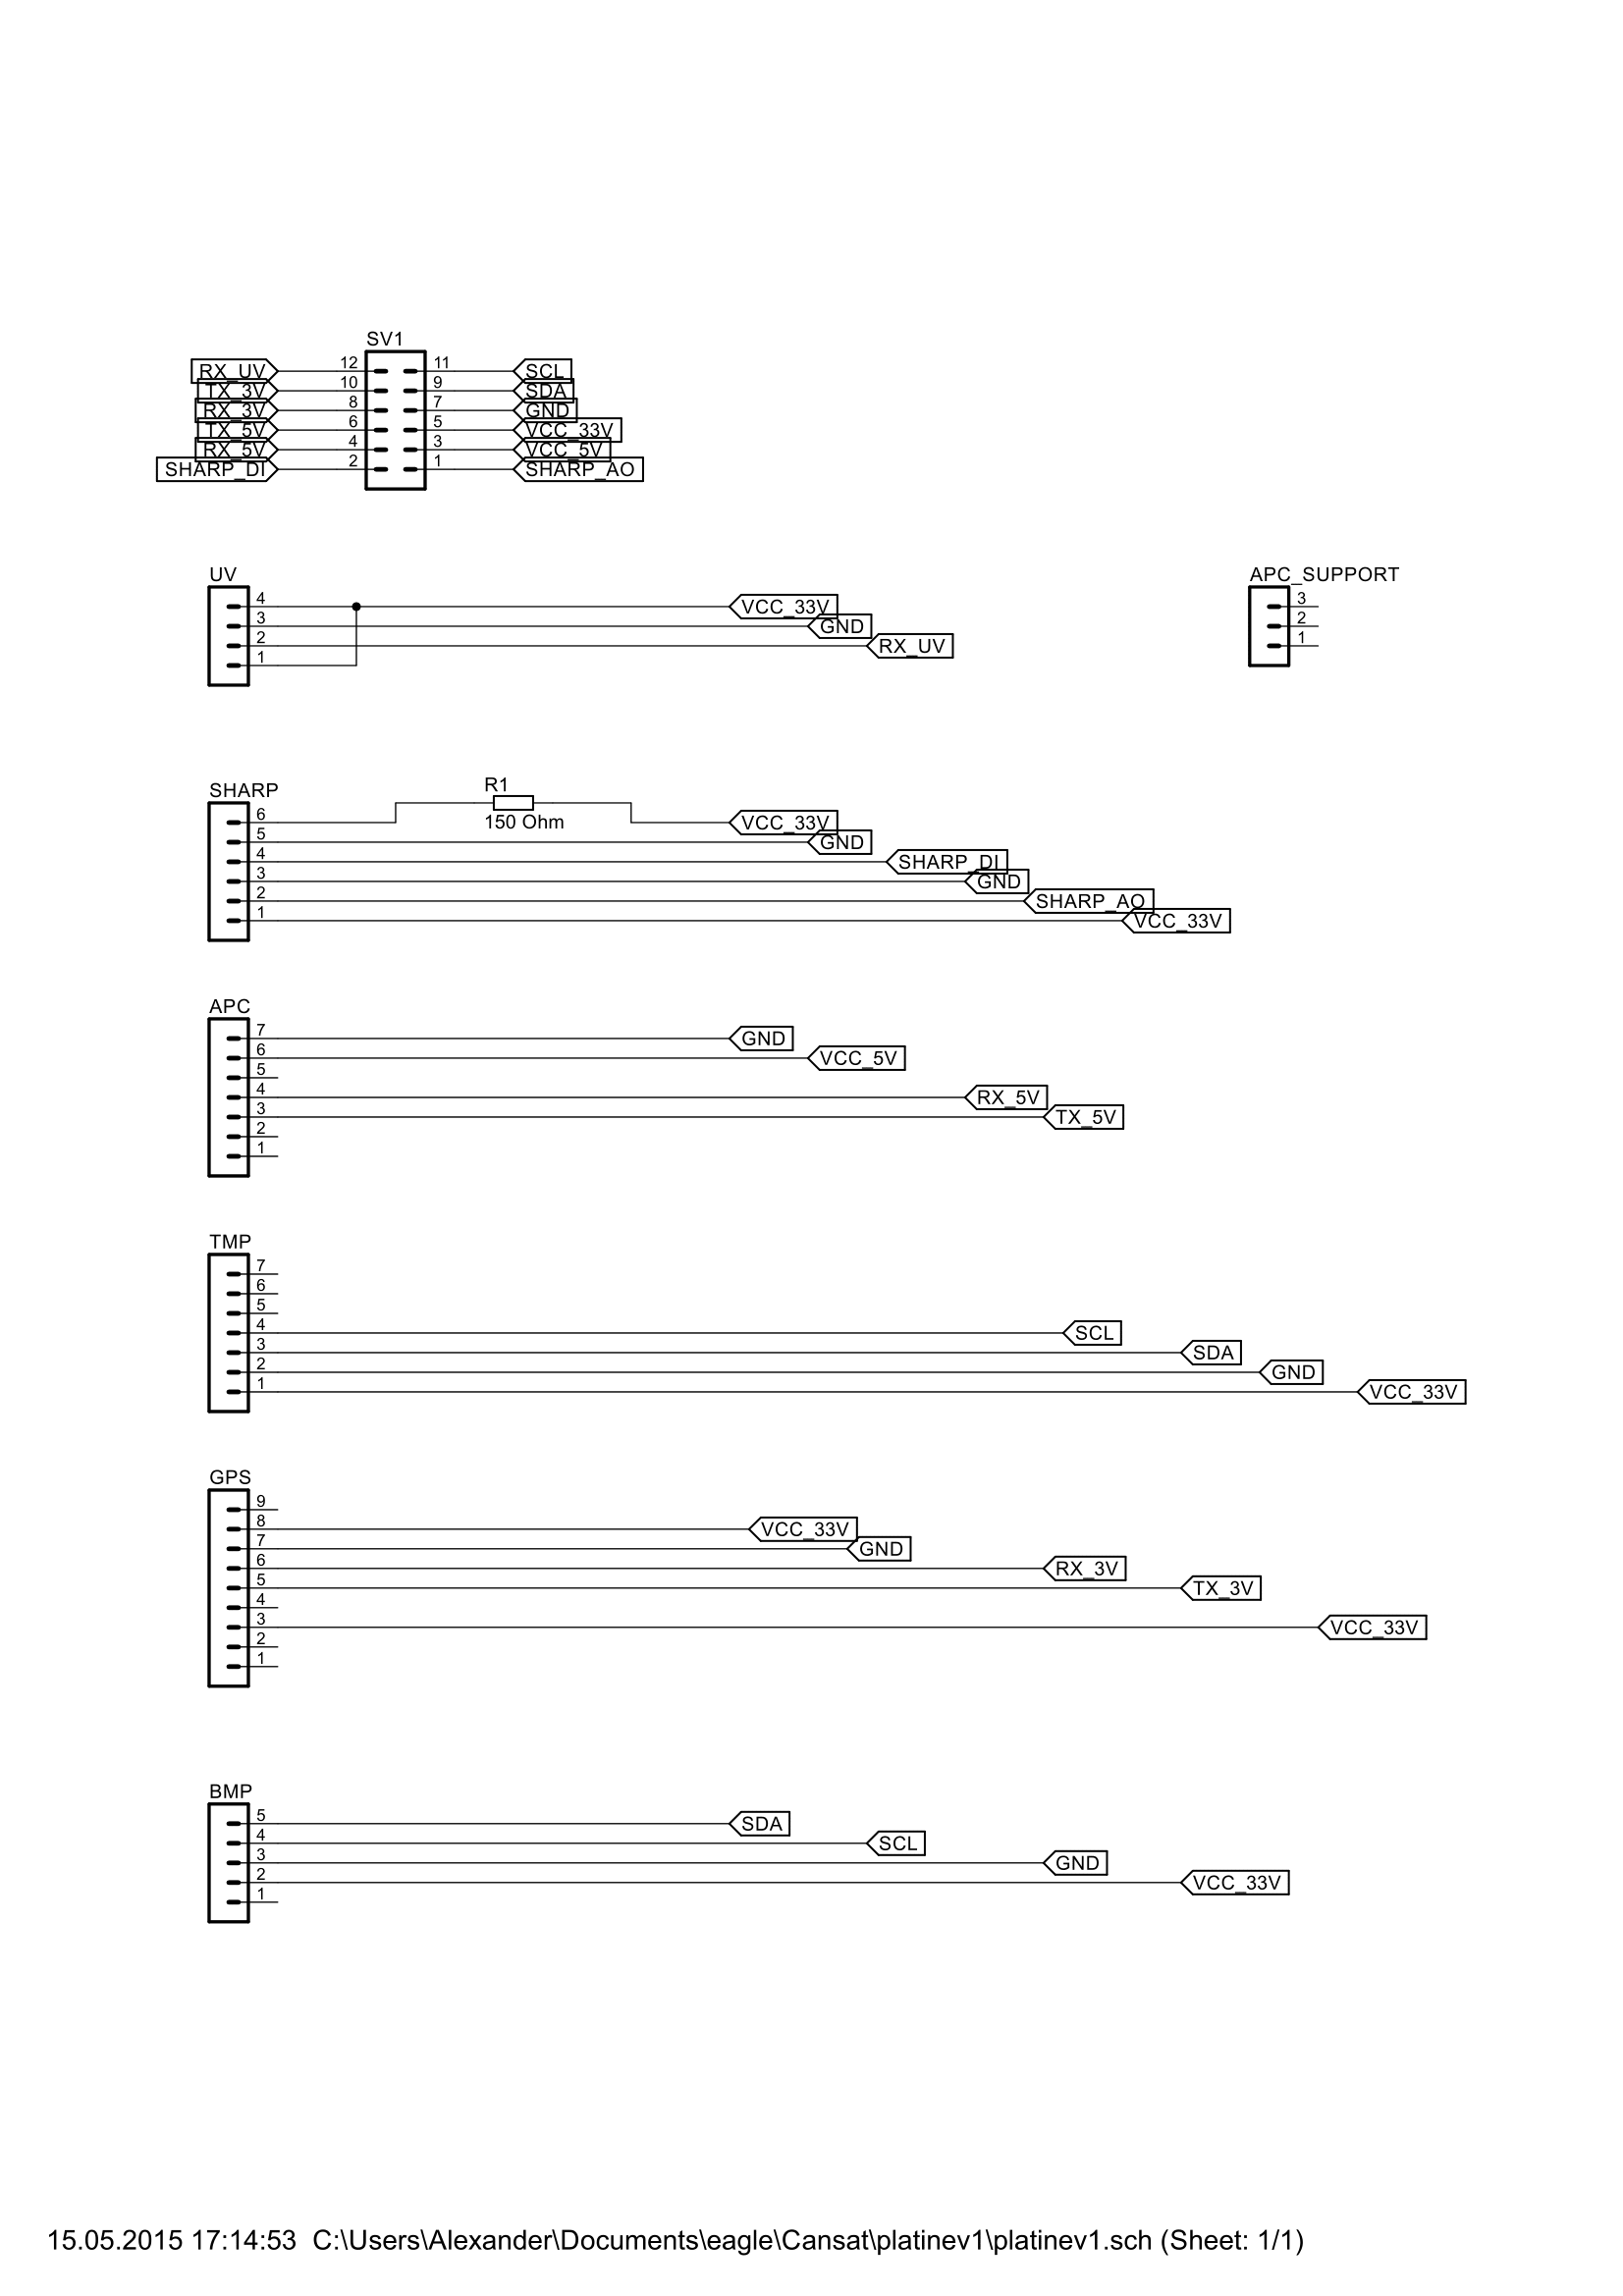
\includegraphics[trim = 60mm 100mm 55mm 100mm, clip, width=0.8\textwidth]{8_Anhang/Schaltplanv1.png}
	\caption{Der Schaltplan der Sensorik Platine}
	\label{pic_schaltplan}
\end{figure}

\newpage

\begin{figure}[H]
	\centering
	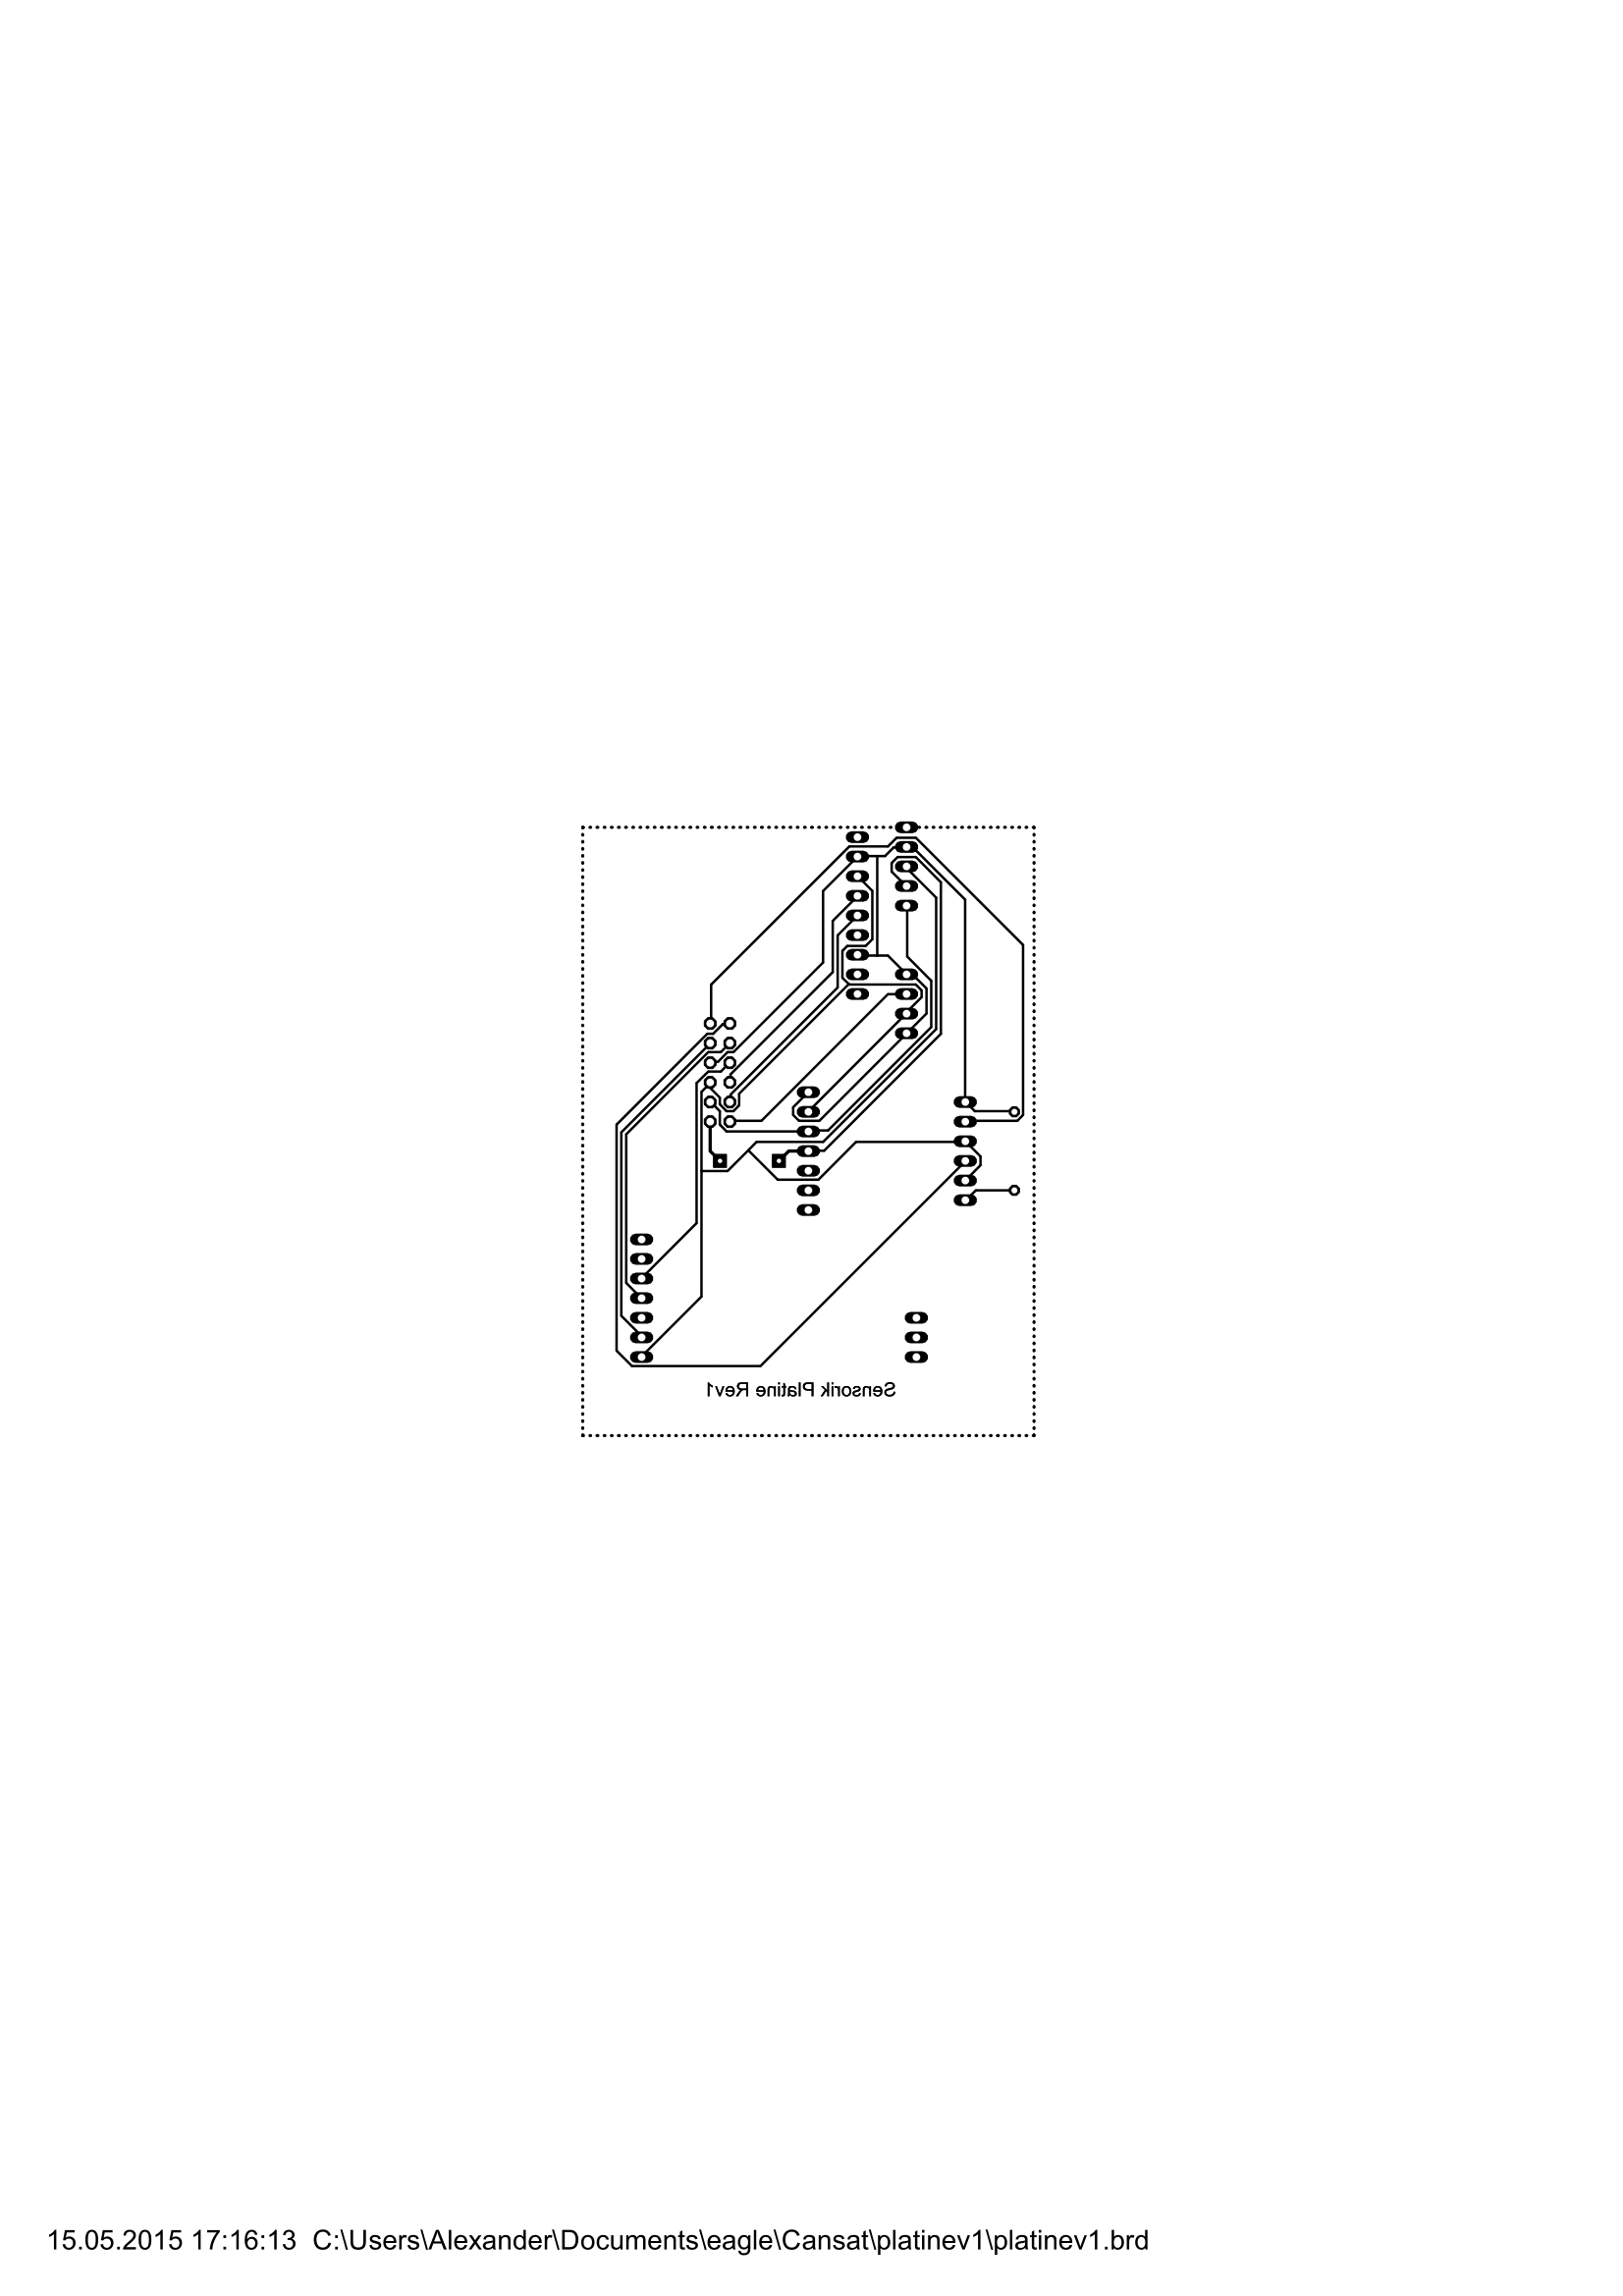
\includegraphics[trim = 200mm 300mm 200mm 280mm, clip,width=0.8\textwidth]{8_Anhang/Layoutv1.png}
	\caption{Das Layout der Sensorik Platine}
	\label{pic_layout}
\end{figure}

\newpage

\begin{figure}[H]
	\centering
	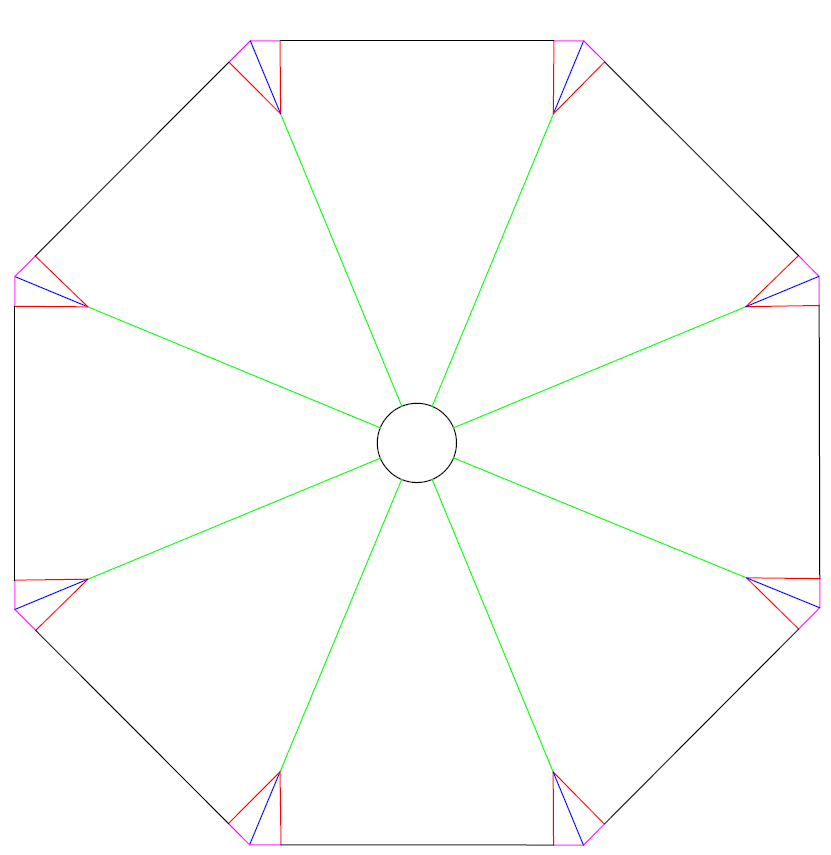
\includegraphics[ width=0.8\textwidth]{8_Anhang/fallschirmSkizze.PNG}
	\caption{Skizze des Fallschirms}
	\label{pic_fallschrimskizze}
\end{figure}

\newpage

\subsection{Bodenstationsarchitektur}
\begin{figure}[H]
	\centering
	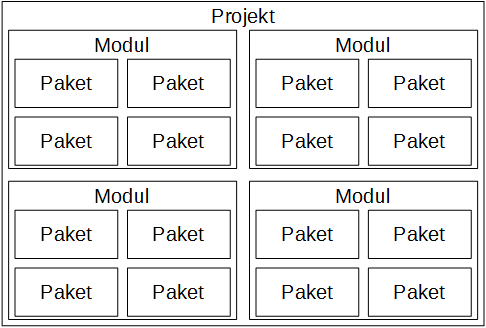
\includegraphics[width=0.8\textwidth]{3_Beschreibung_der_Bodenstation/NBP_Modularchitektur.png}
	\caption{Modularchitektur von Netbeans Platform}
	\label{nbp_modularchitektur}
\end{figure}

\begin{figure}[H]
	\centering
	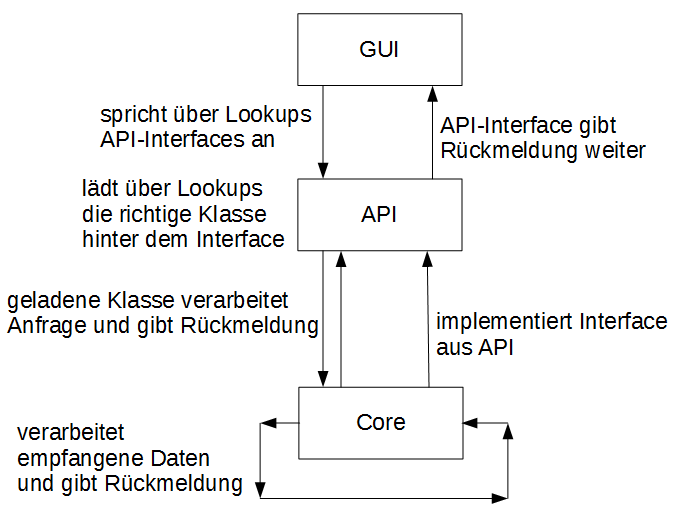
\includegraphics[width=0.8\textwidth]{3_Beschreibung_der_Bodenstation/Bodenstation_Modularchitektur.png}
	\caption{Modularchitektur der Bodenstation}
	\label{station_modularchitektur}
\end{figure}
\vspace{-5cm}

\newpage

\begin{figure}[H]
	\centering
	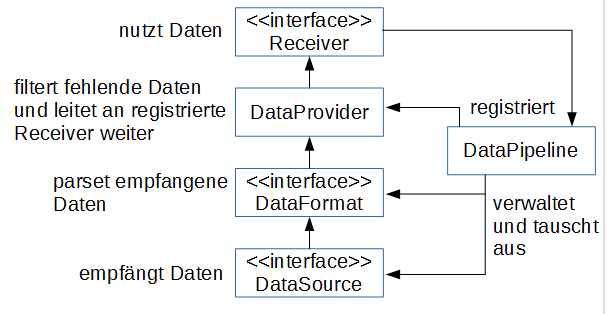
\includegraphics[width=0.8\textwidth]{3_Beschreibung_der_Bodenstation/Input-Pipeline_Architektur.png}
	\caption{Architektur der Input-Pipeline}
	\label{inputpipeline}
\end{figure}

\newpage
\subsection{Protokolle}
Auf den nachfolgenden Seiten finden sich Protokolle diverser Meetings. Diese Protokolle wurden mal mit mehr, und mal mit weniger Mühe und Aufwand angefertigt. Uns war lediglich wichtig, dass es Protokolle gibt, an denen wir unsere Arbeit belegen können, und an denen bereits getroffene Entscheidungen nachvollzogen werden können.

\includepdf[pages=-]{8_Anhang/Protokolle/140625_Meeting_Protokoll}%

\newpage
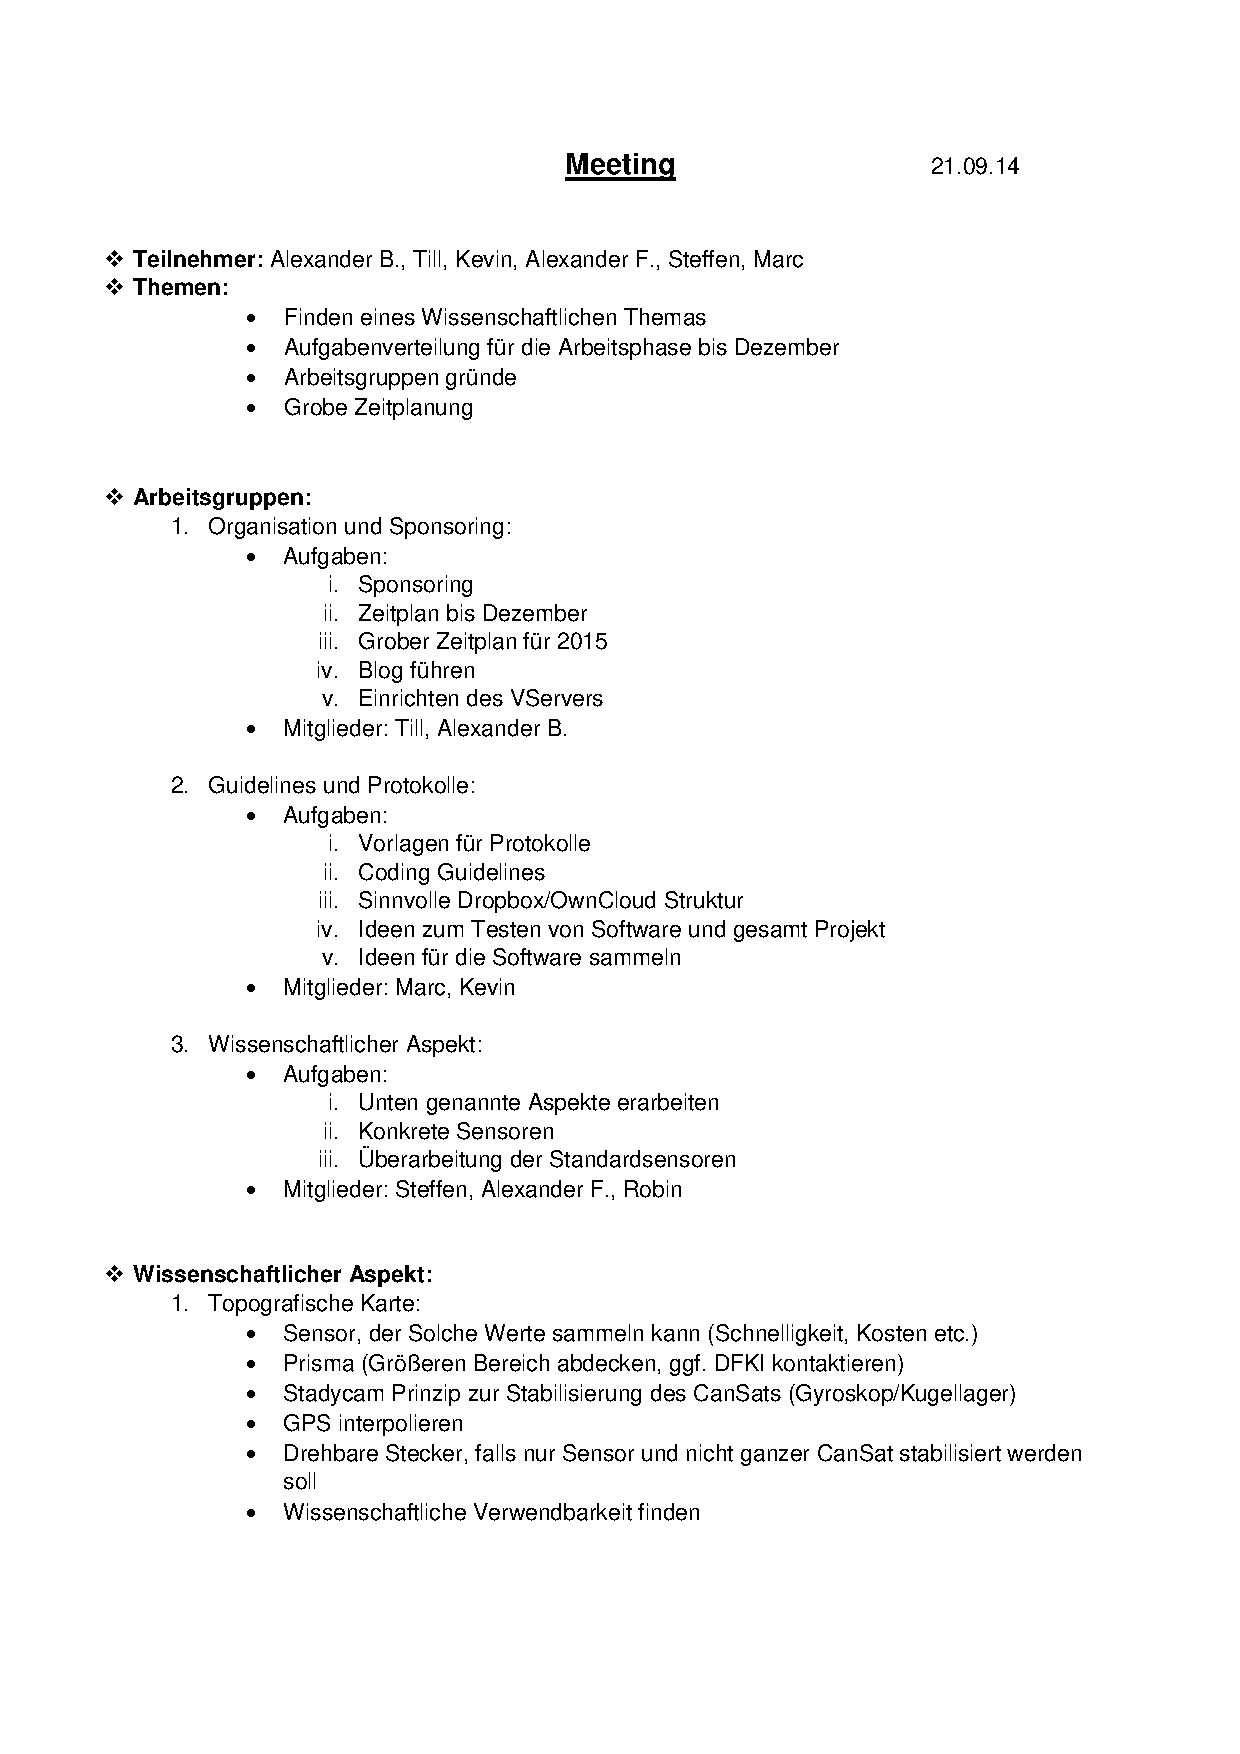
\includepdf[pages=-]{8_Anhang/Protokolle/140921_Meeting_Protokoll}%

\newpage
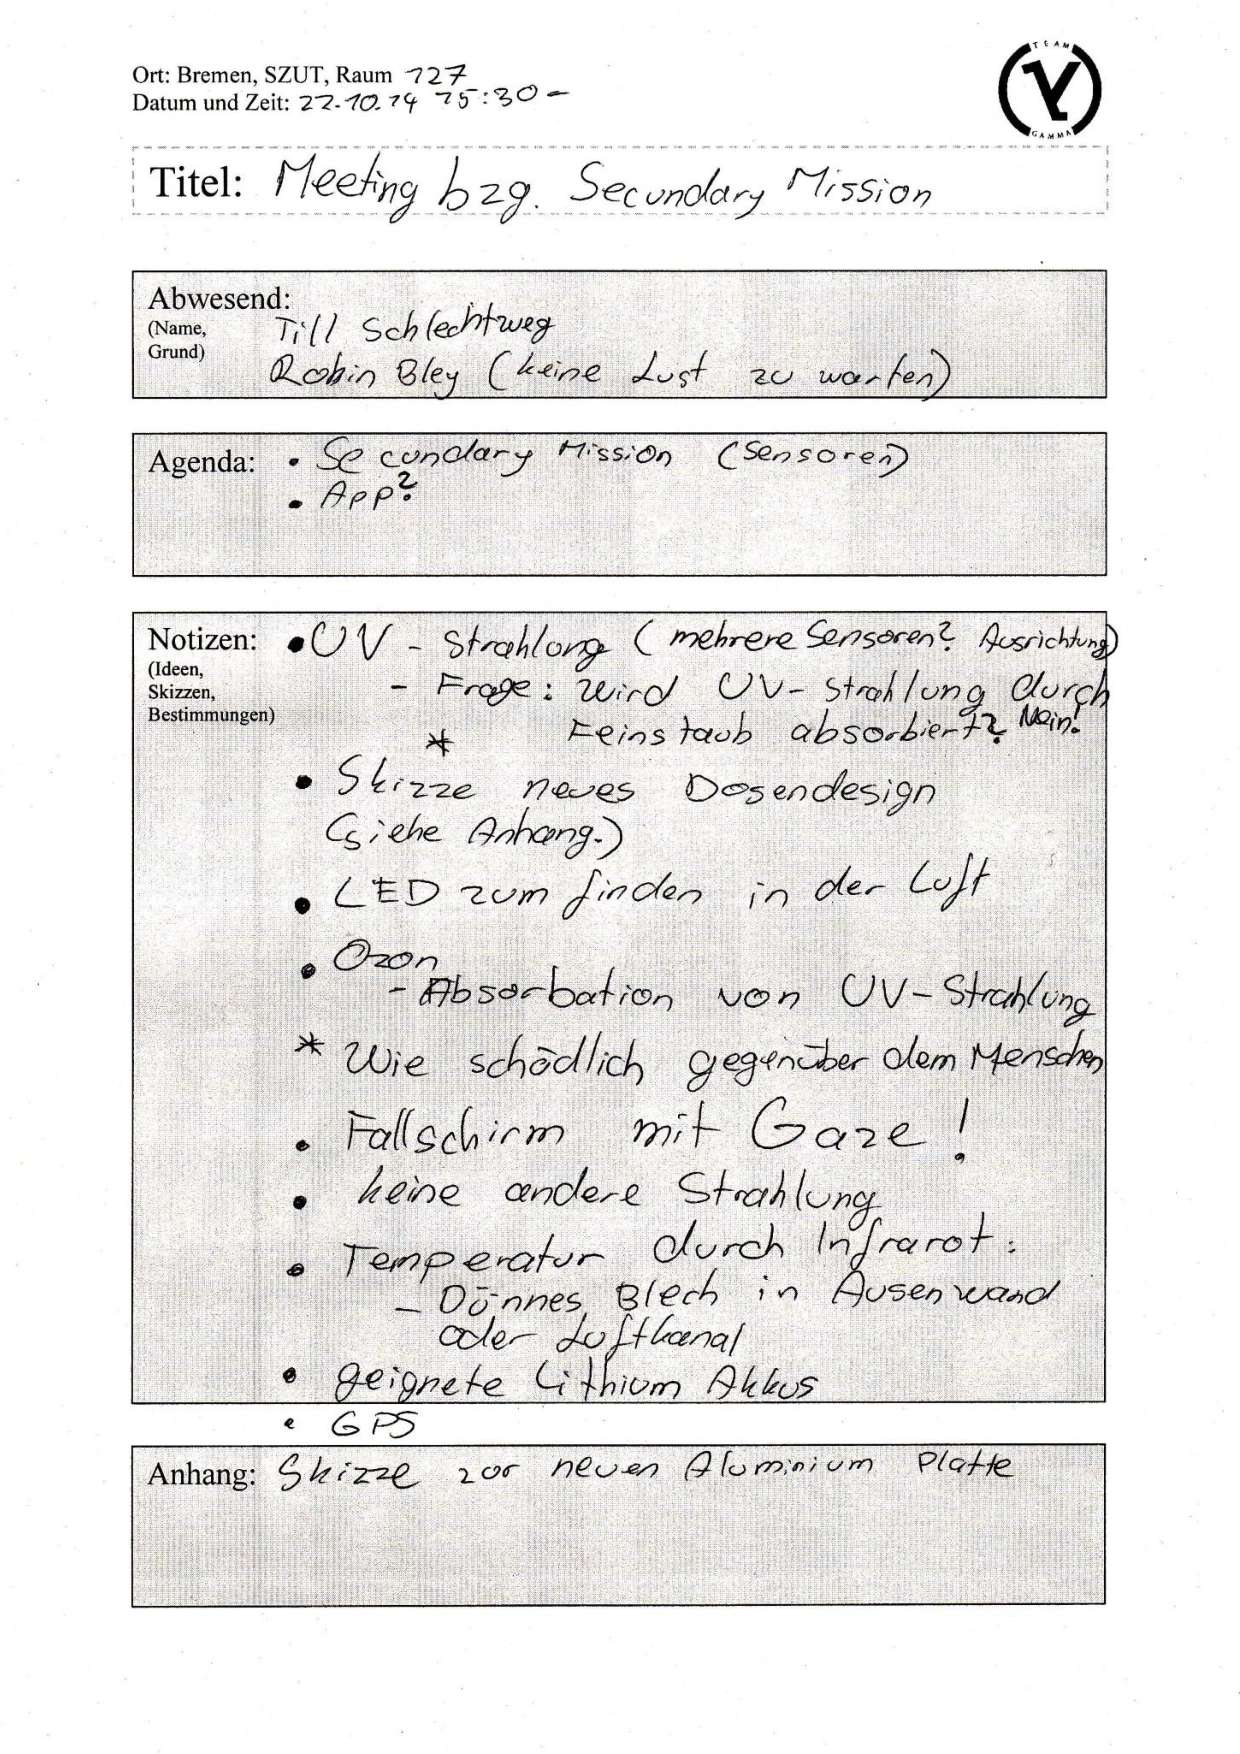
\includepdf[pages=-]{8_Anhang/Protokolle/141022_Meeting_Protokoll}%

\newpage
\begin{figure}[H]
	\centering
	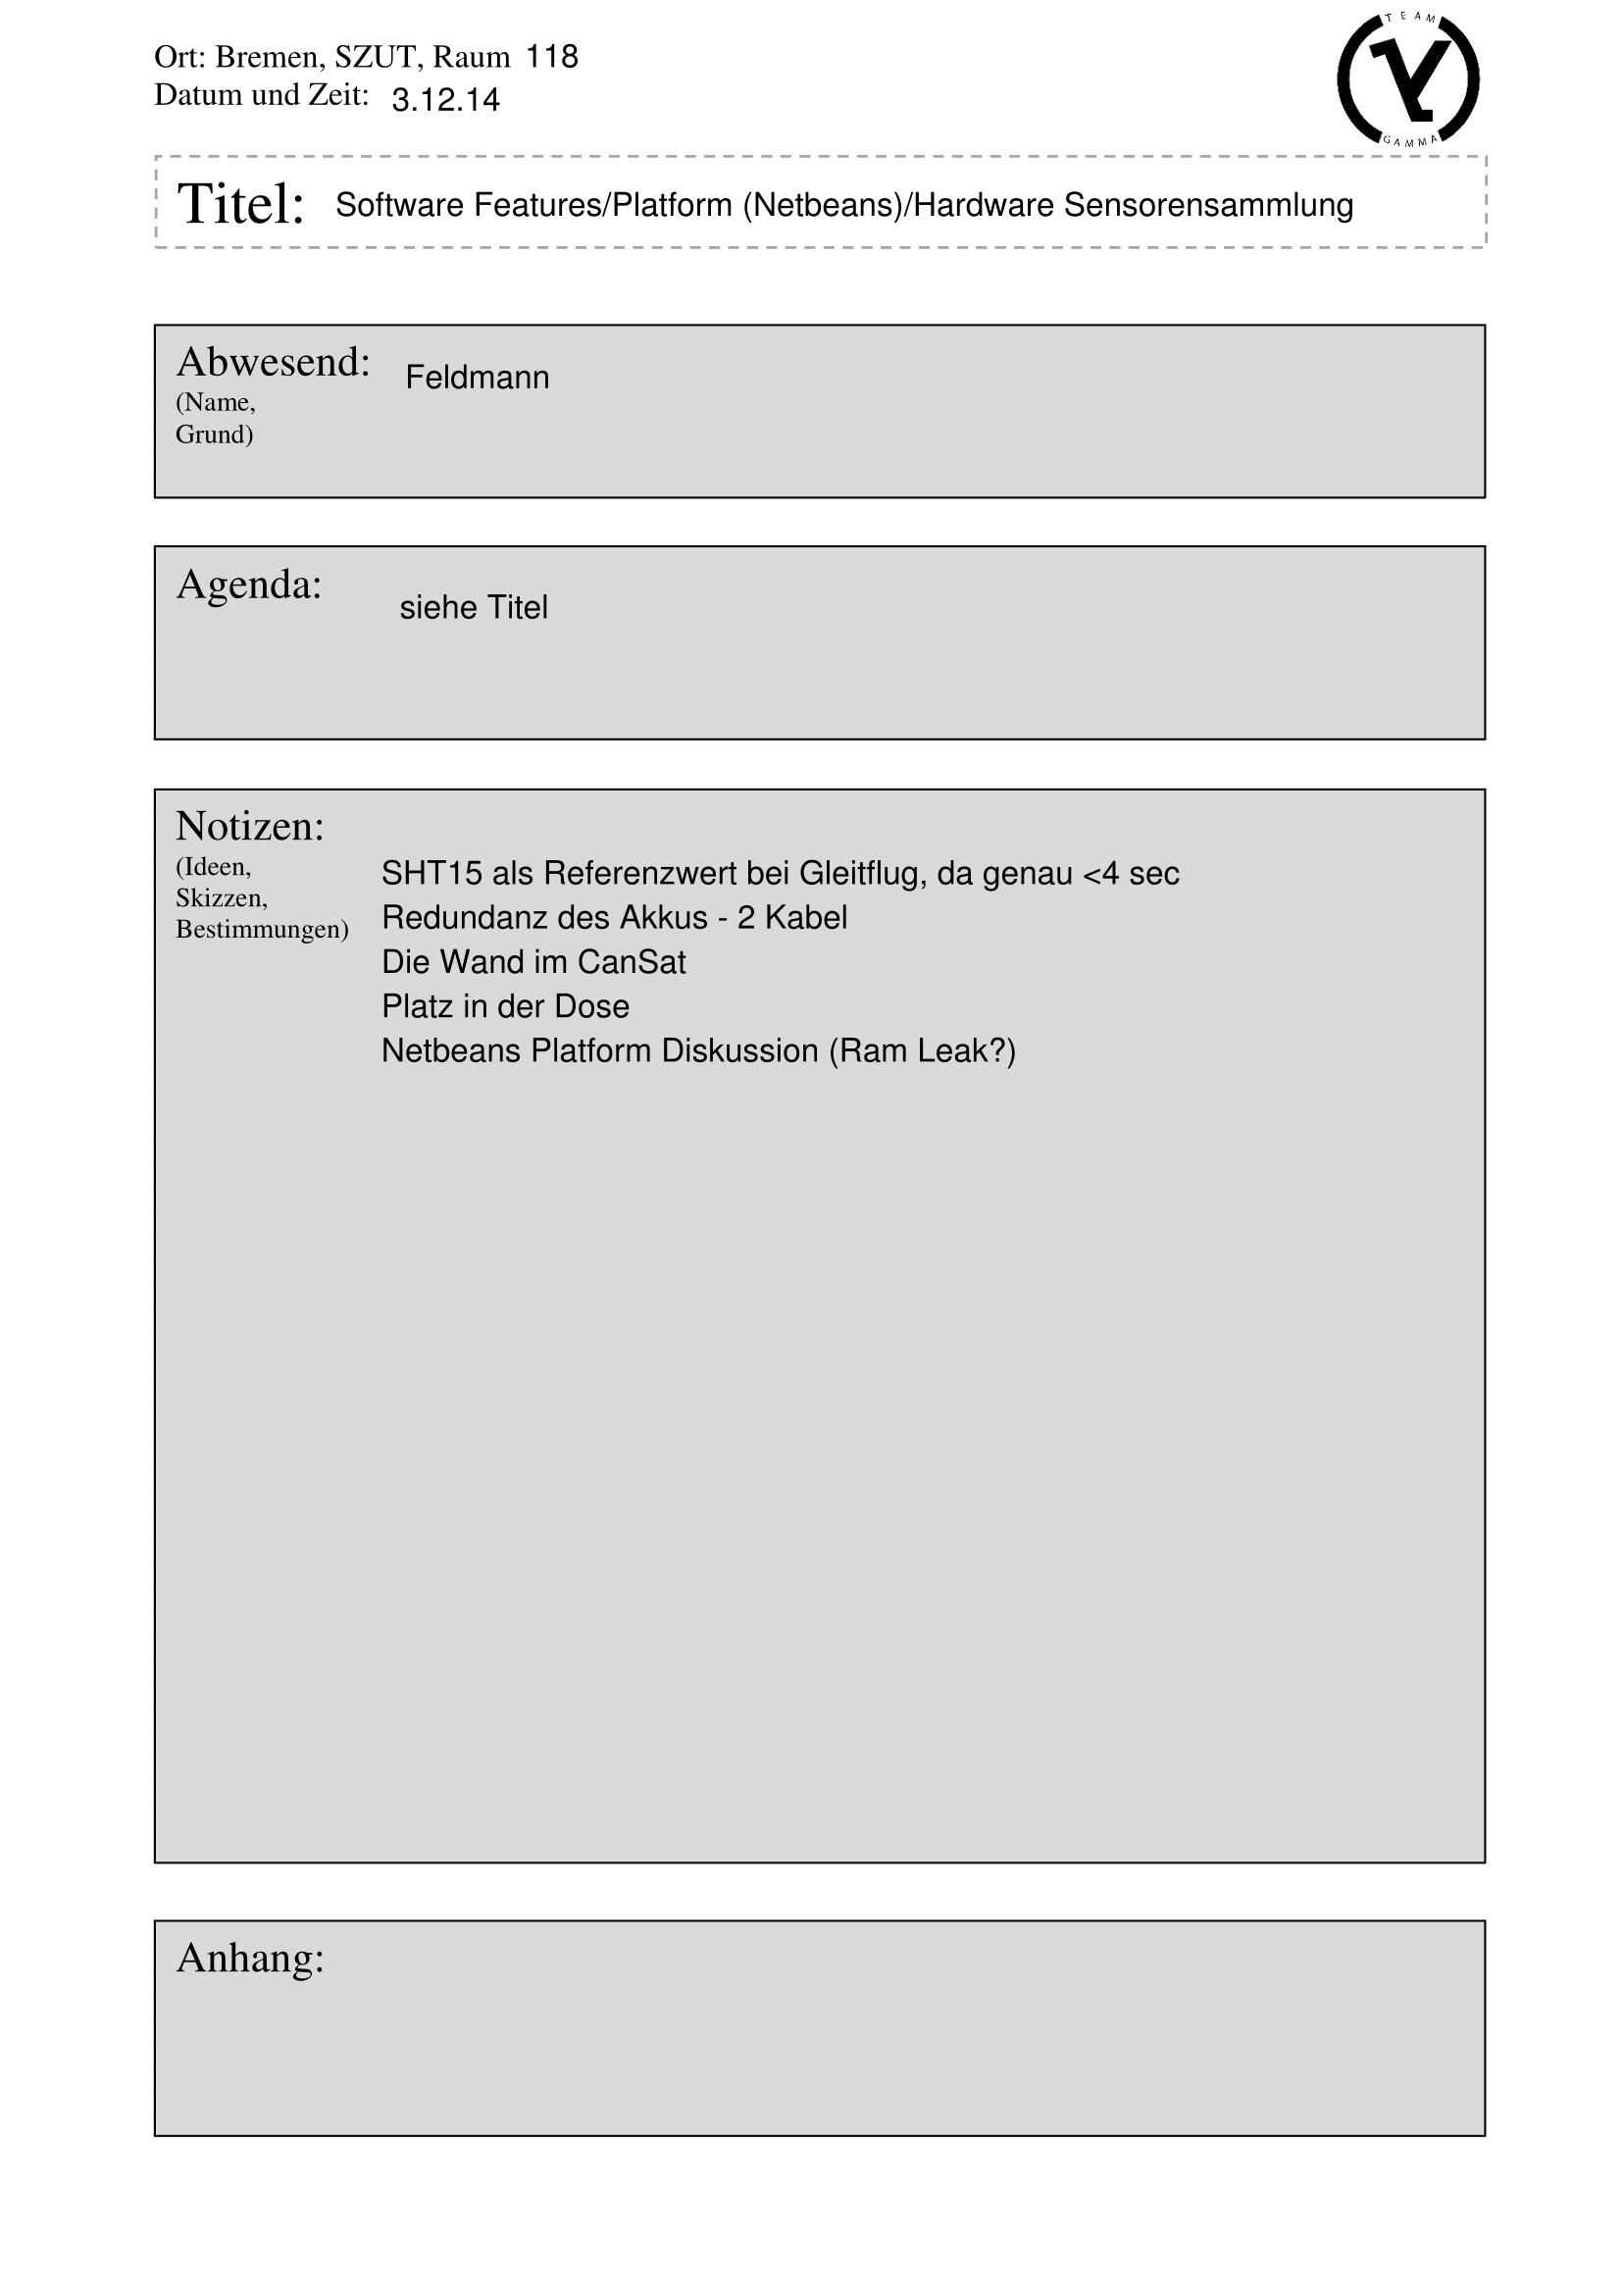
\includegraphics[width=0.8\textwidth]{8_Anhang/Protokolle/141203_Meeting_Protokoll.png}%
	\label{pic_protokoll_140203}
\end{figure}

\newpage
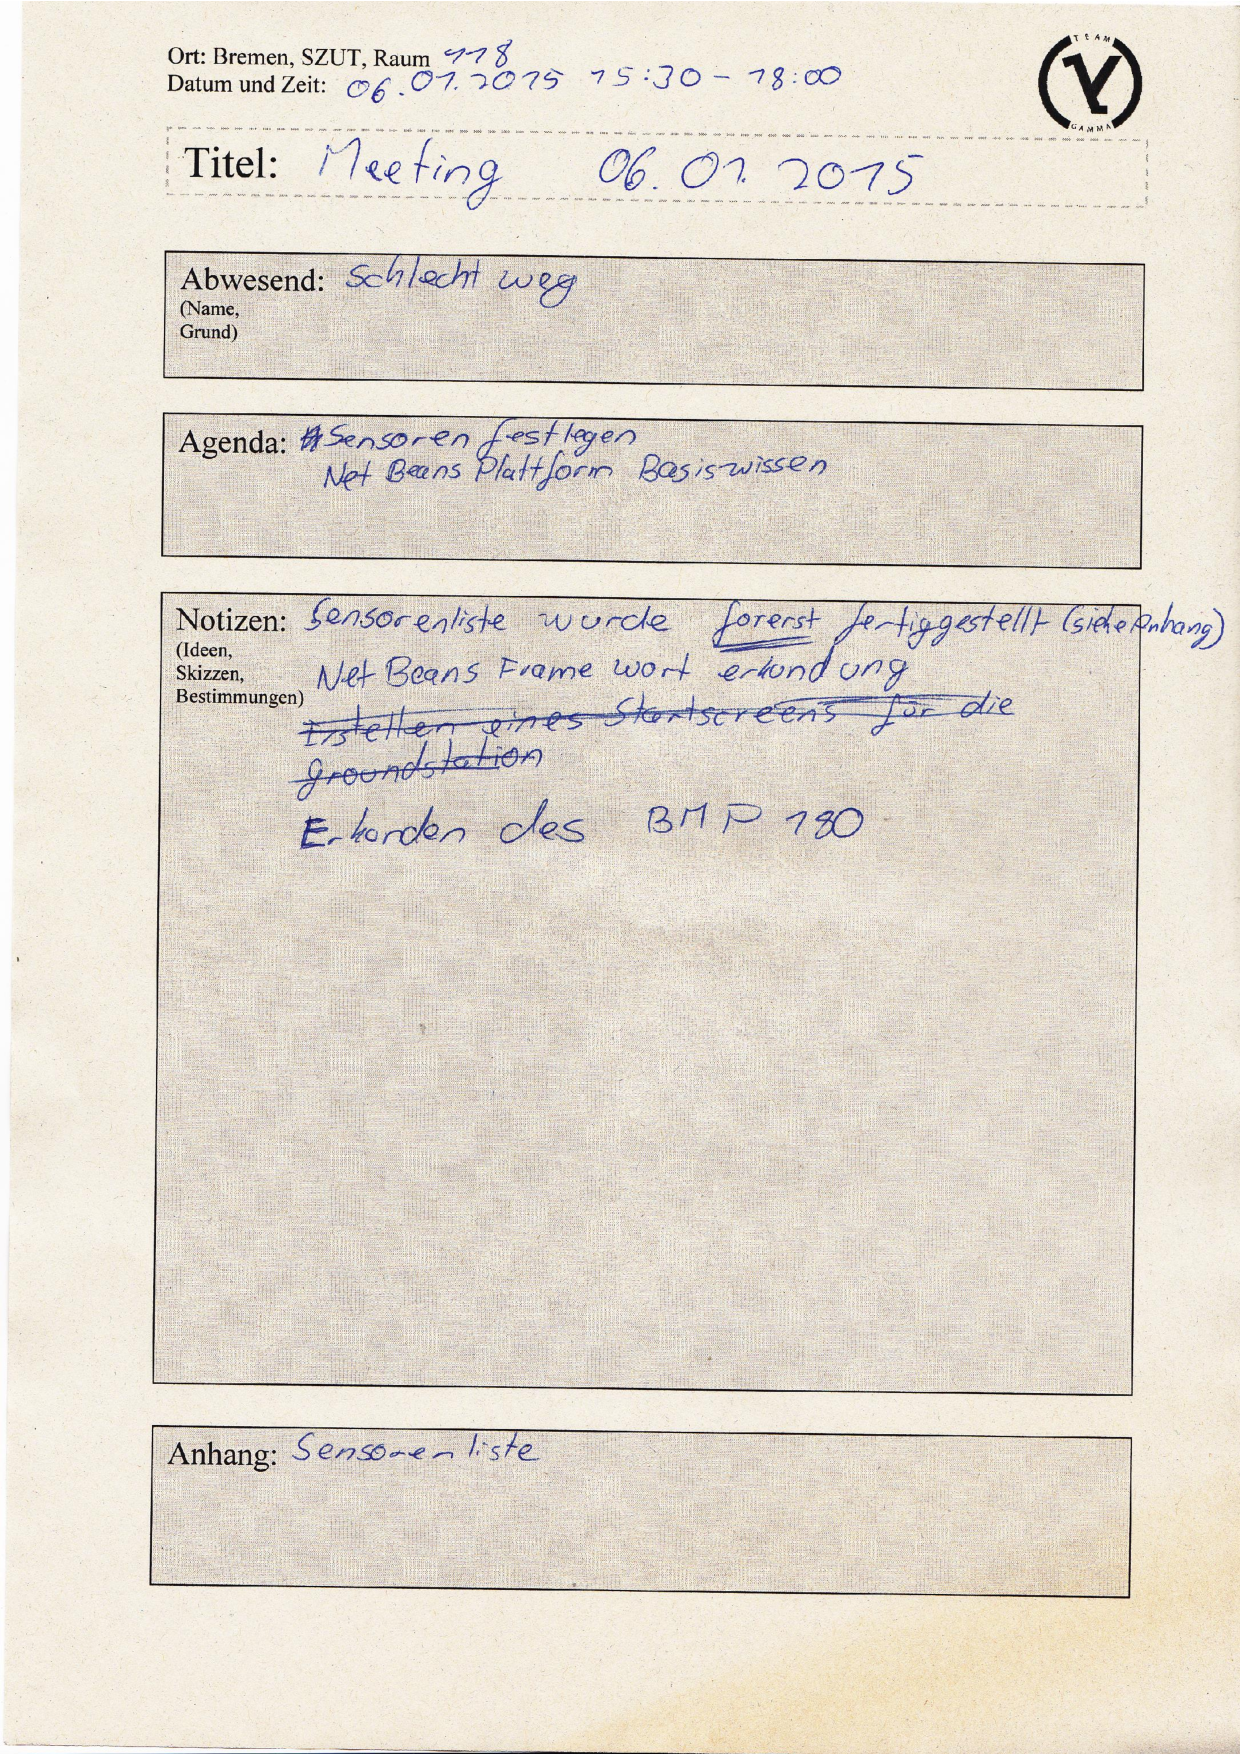
\includepdf{8_Anhang/Protokolle/150106_Meeting_Protokoll}%
\newpage

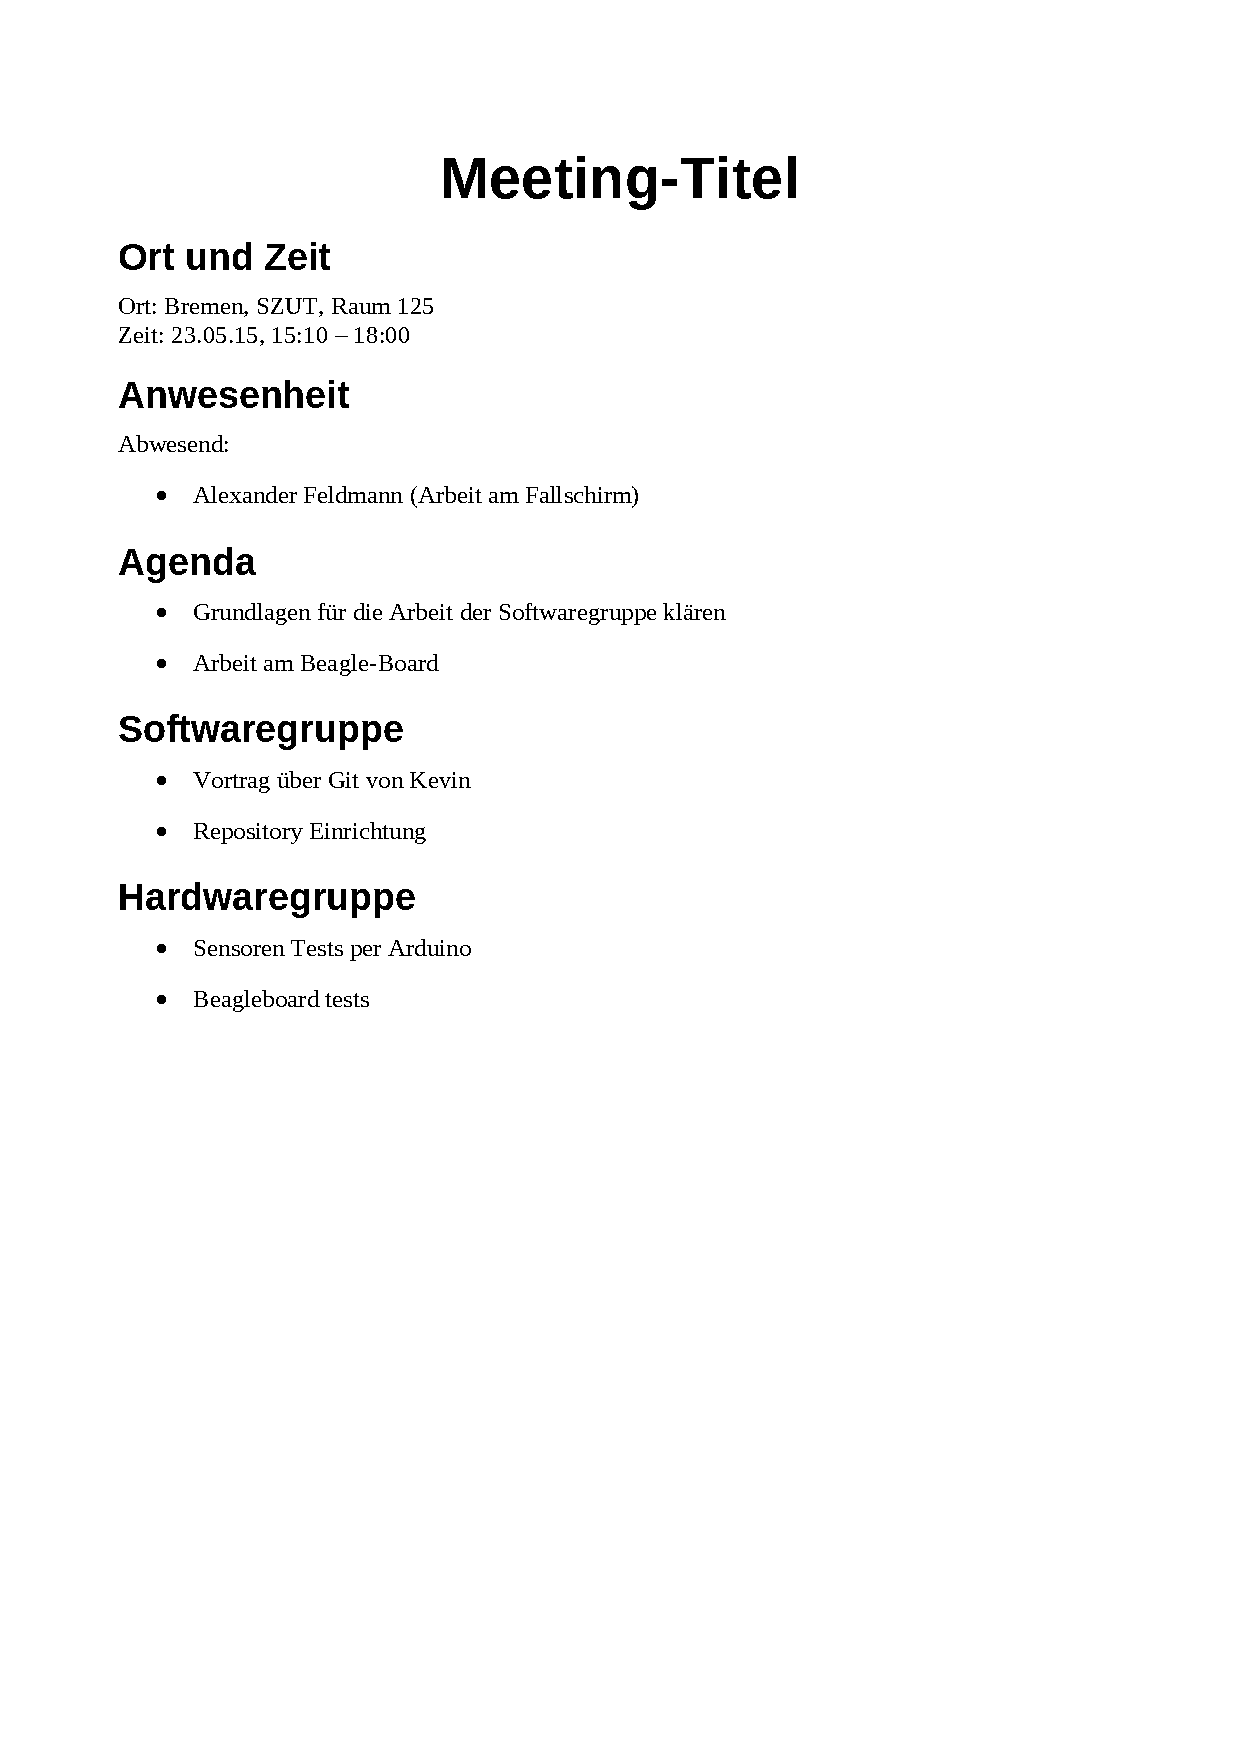
\includepdf{8_Anhang/Protokolle/150204_Meeting_Protokoll}%
\newpage
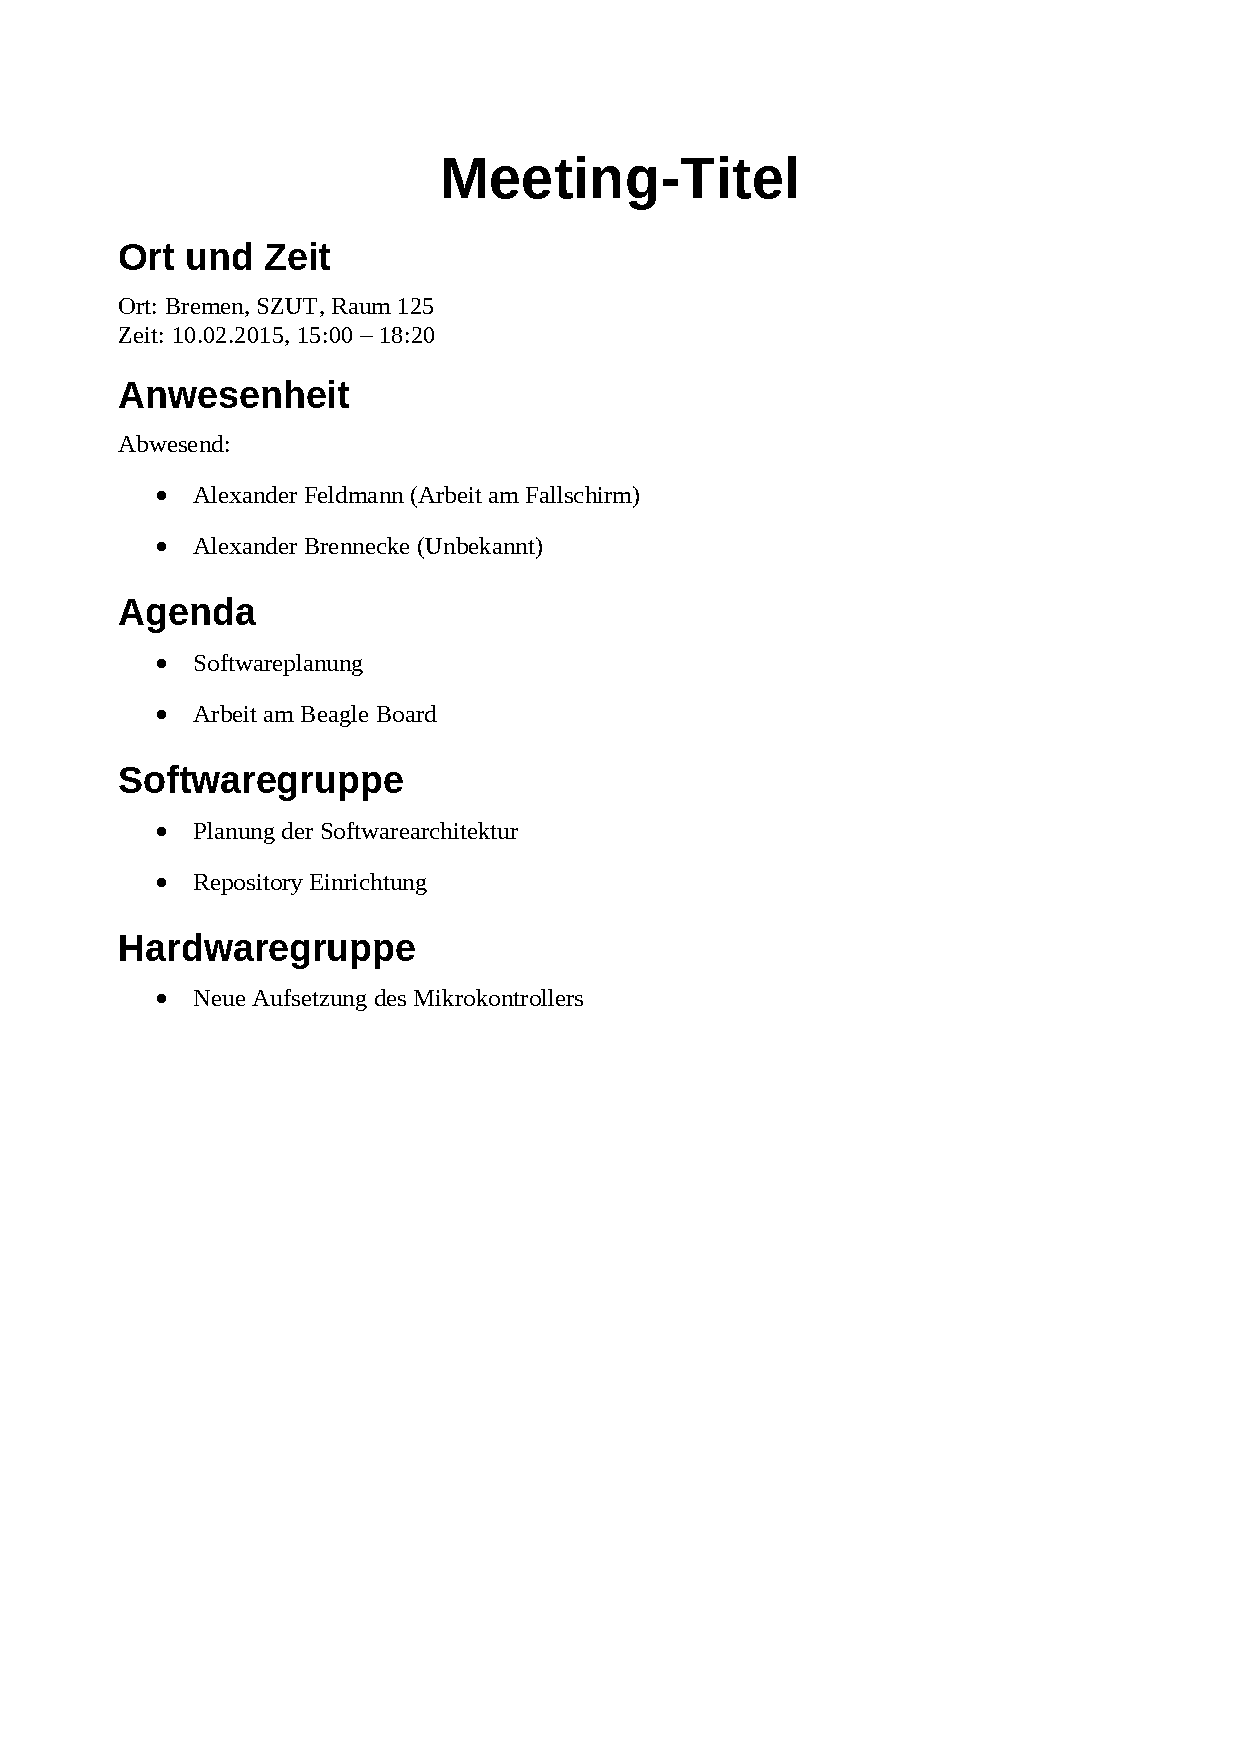
\includepdf{8_Anhang/Protokolle/150210_Meeting_Protokoll}%
\newpage
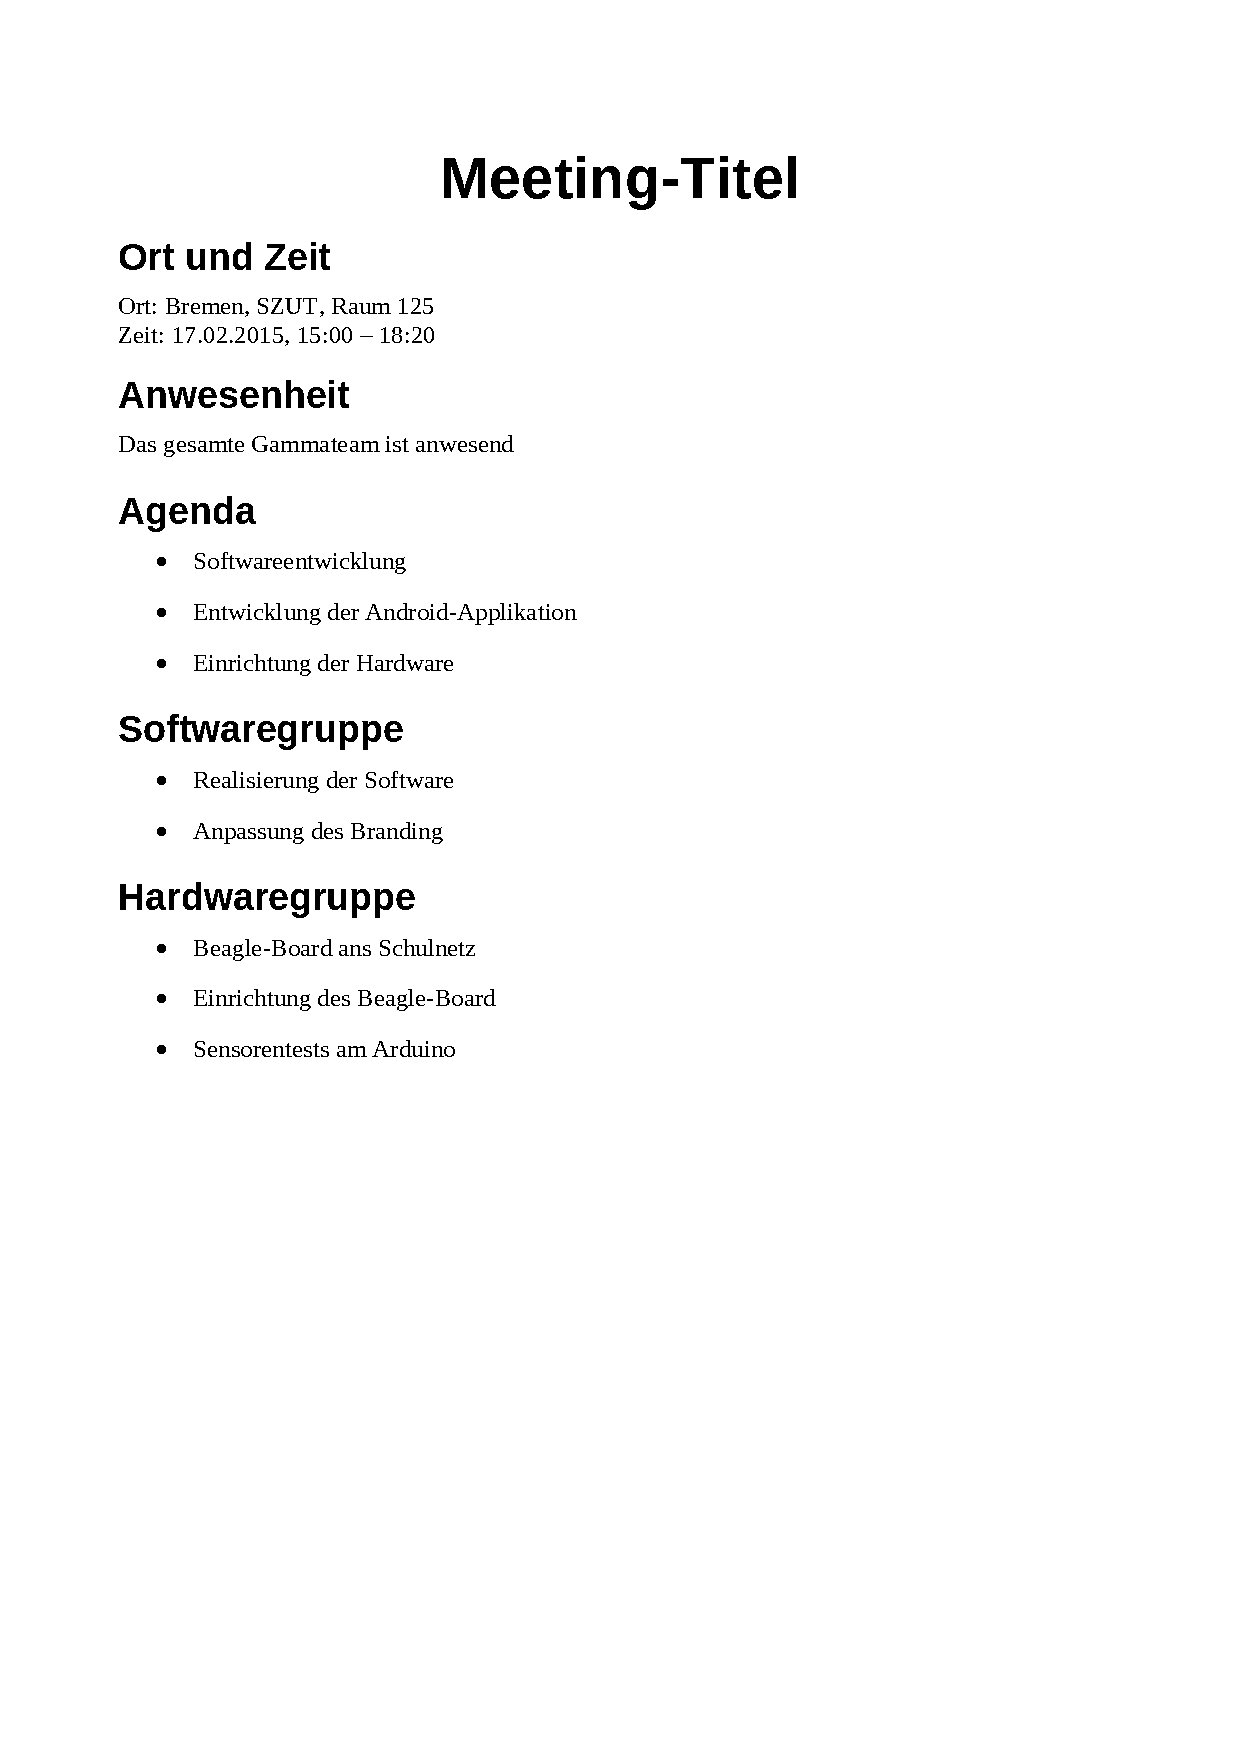
\includepdf{8_Anhang/Protokolle/150217_Meeting_Protokoll}%
\newpage
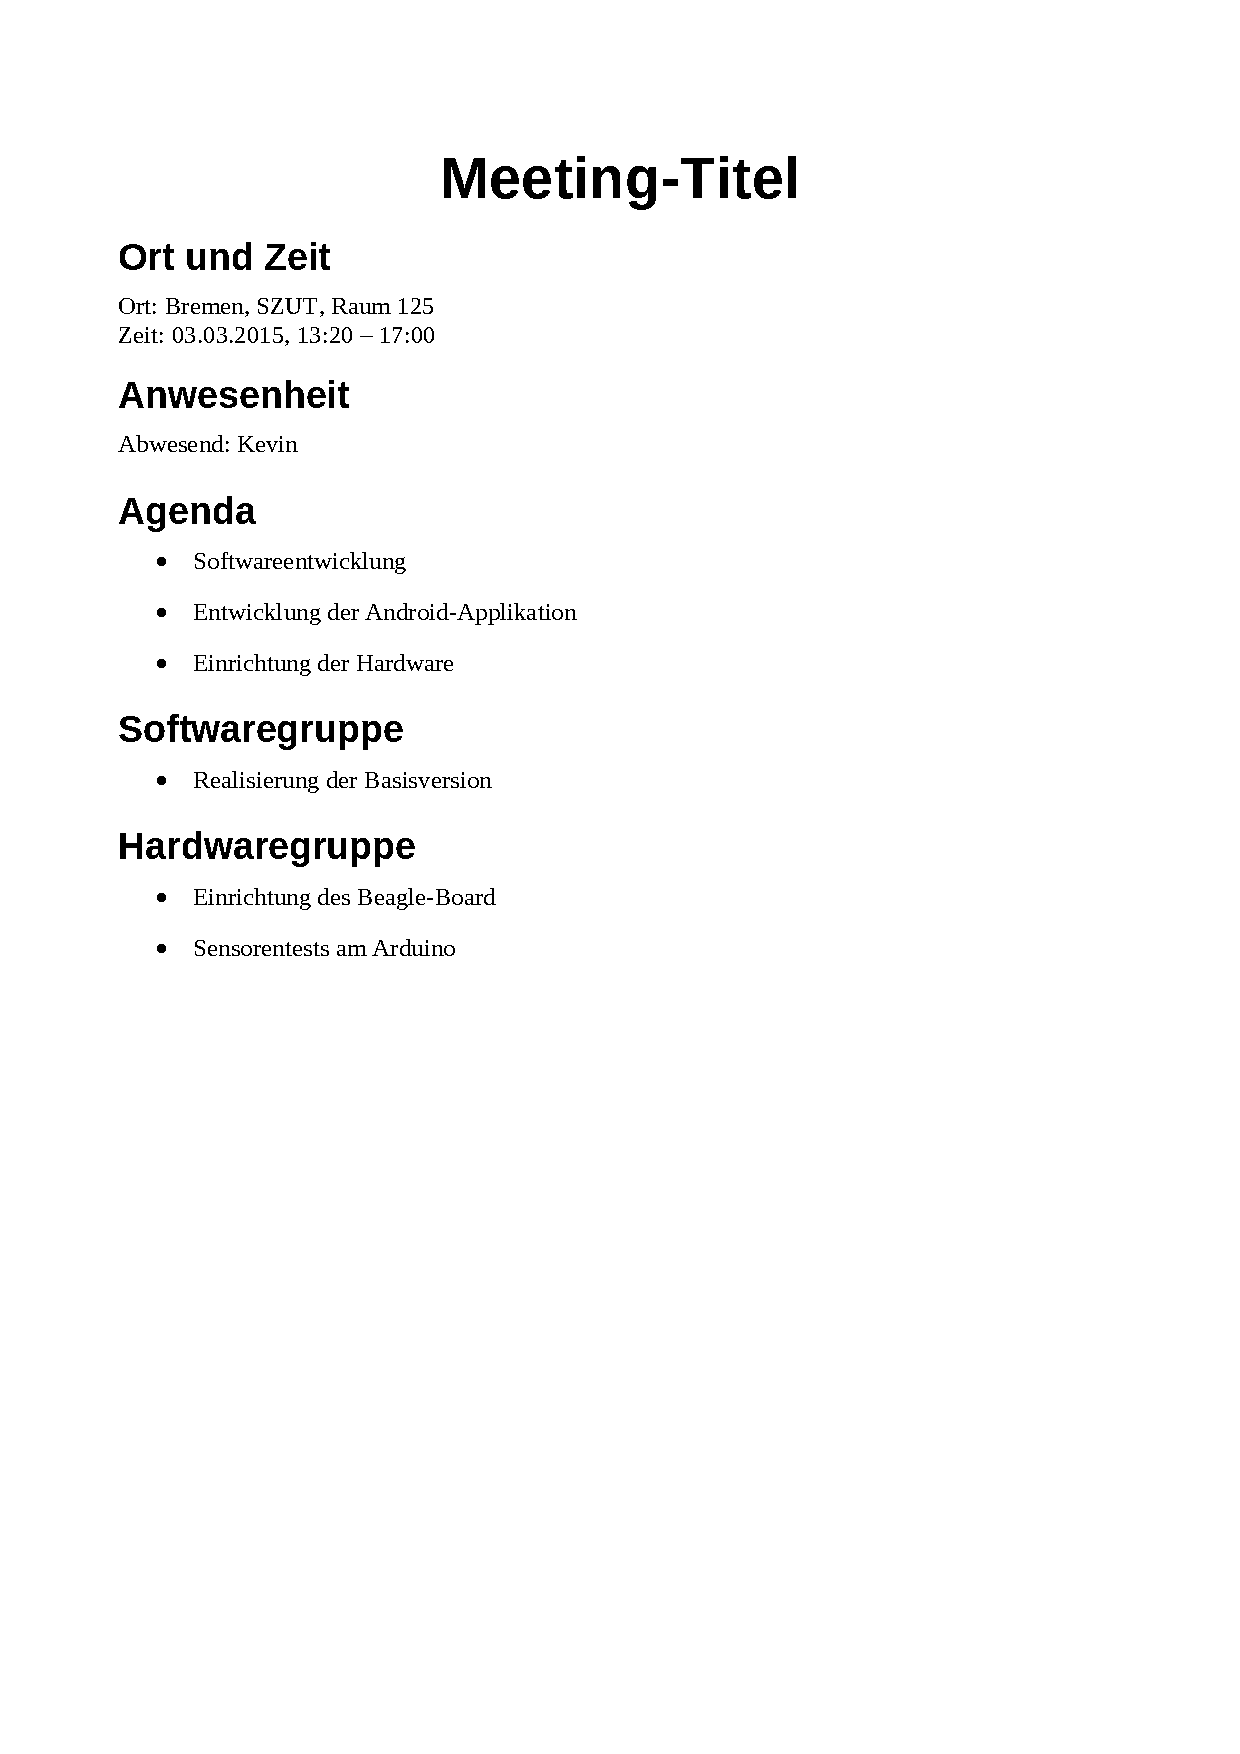
\includepdf{8_Anhang/Protokolle/150303_Meeting_Protokoll}%
\newpage
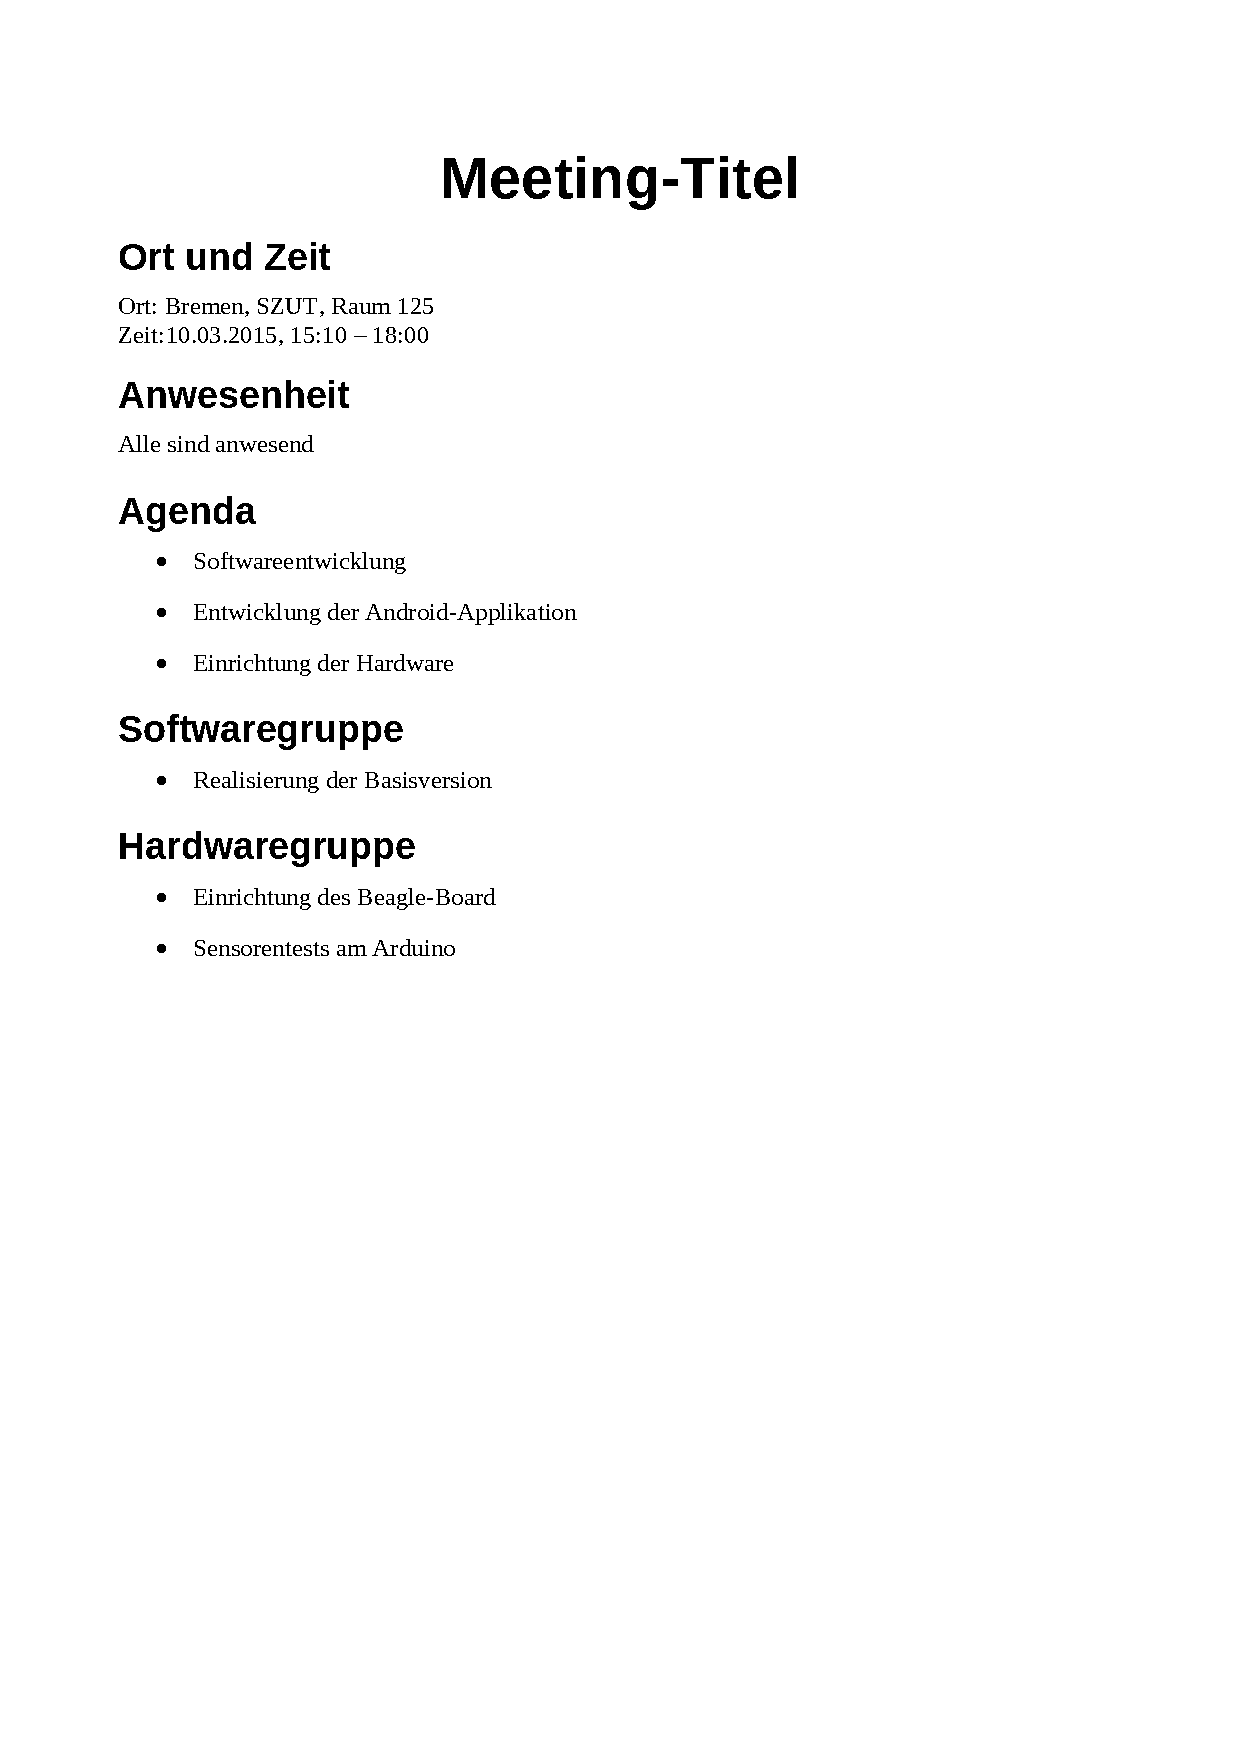
\includepdf{8_Anhang/Protokolle/150310_Meeting_Protokoll}%
\newpage
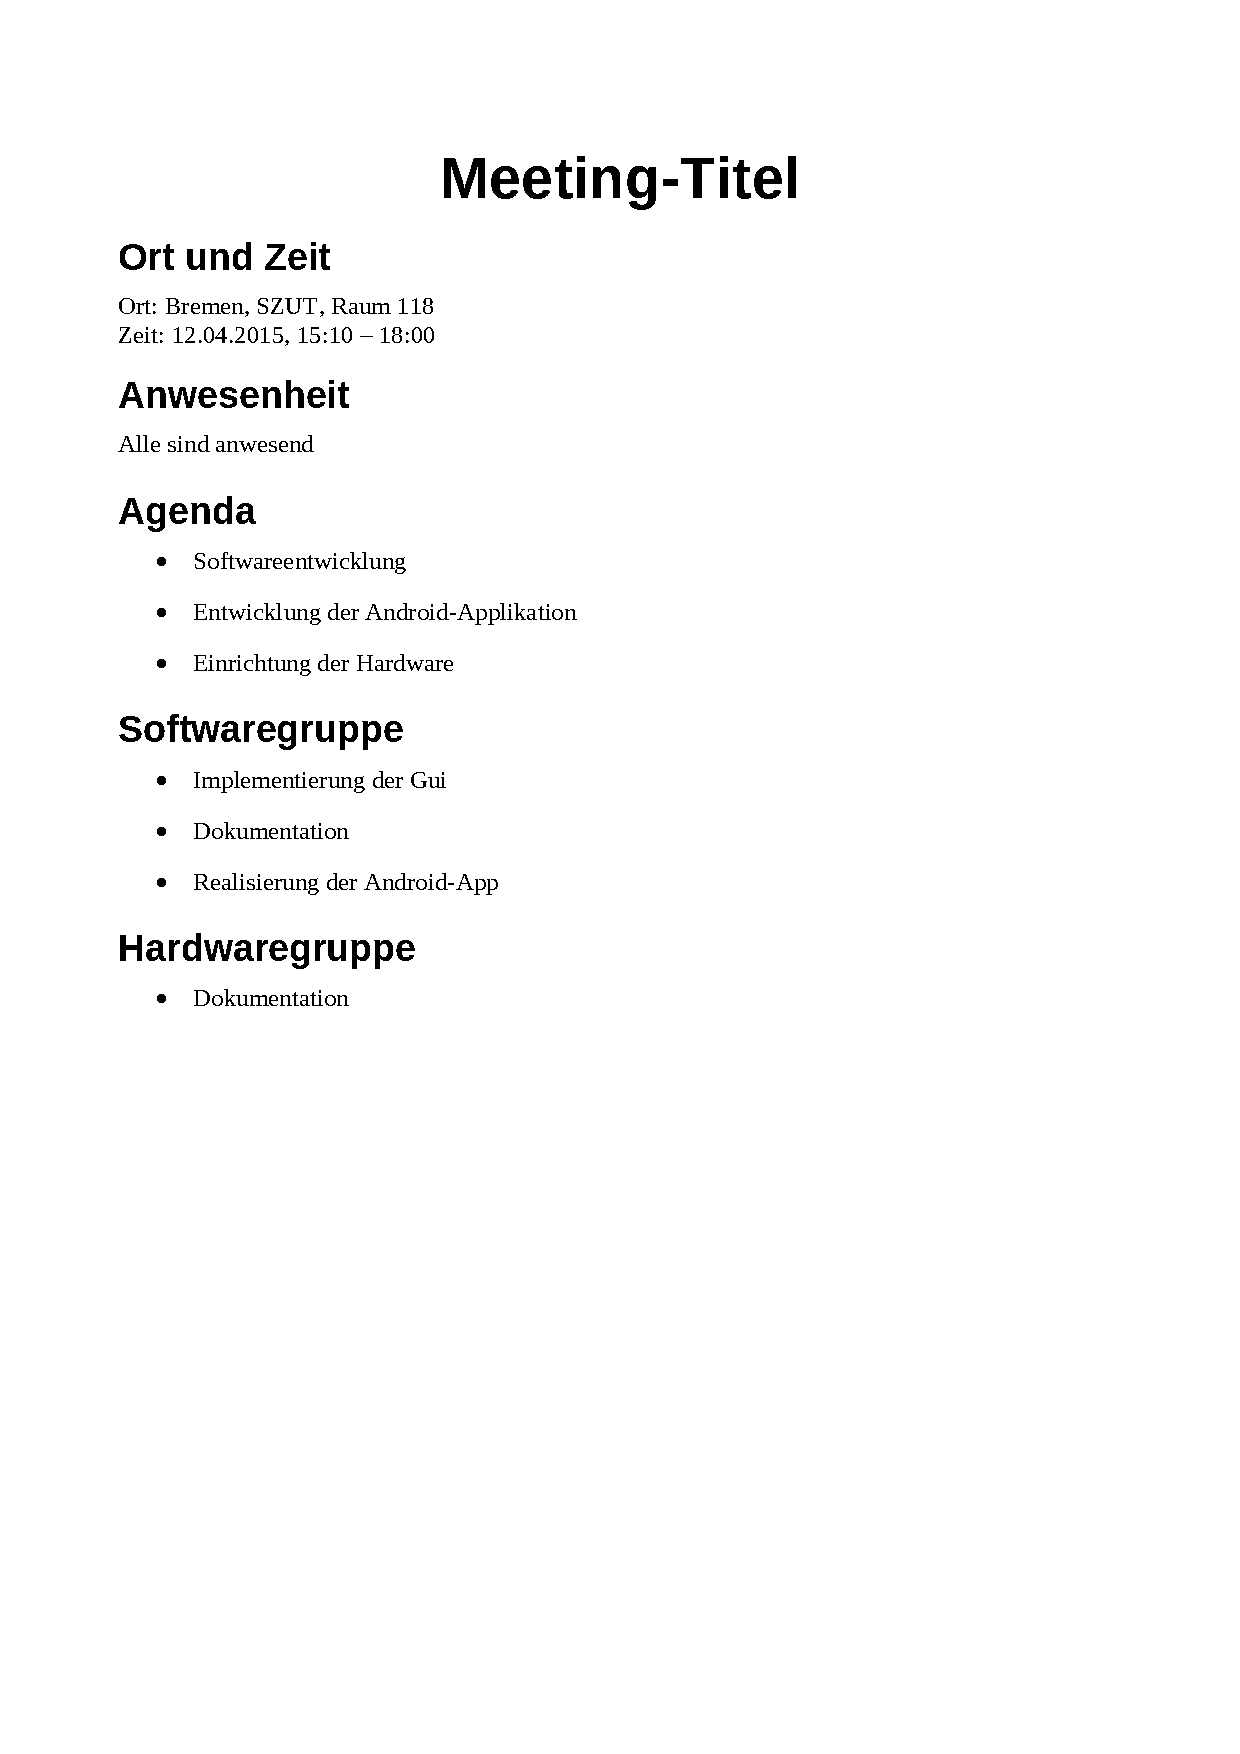
\includepdf{8_Anhang/Protokolle/150317_Meeting_Protokoll}%
\newpage
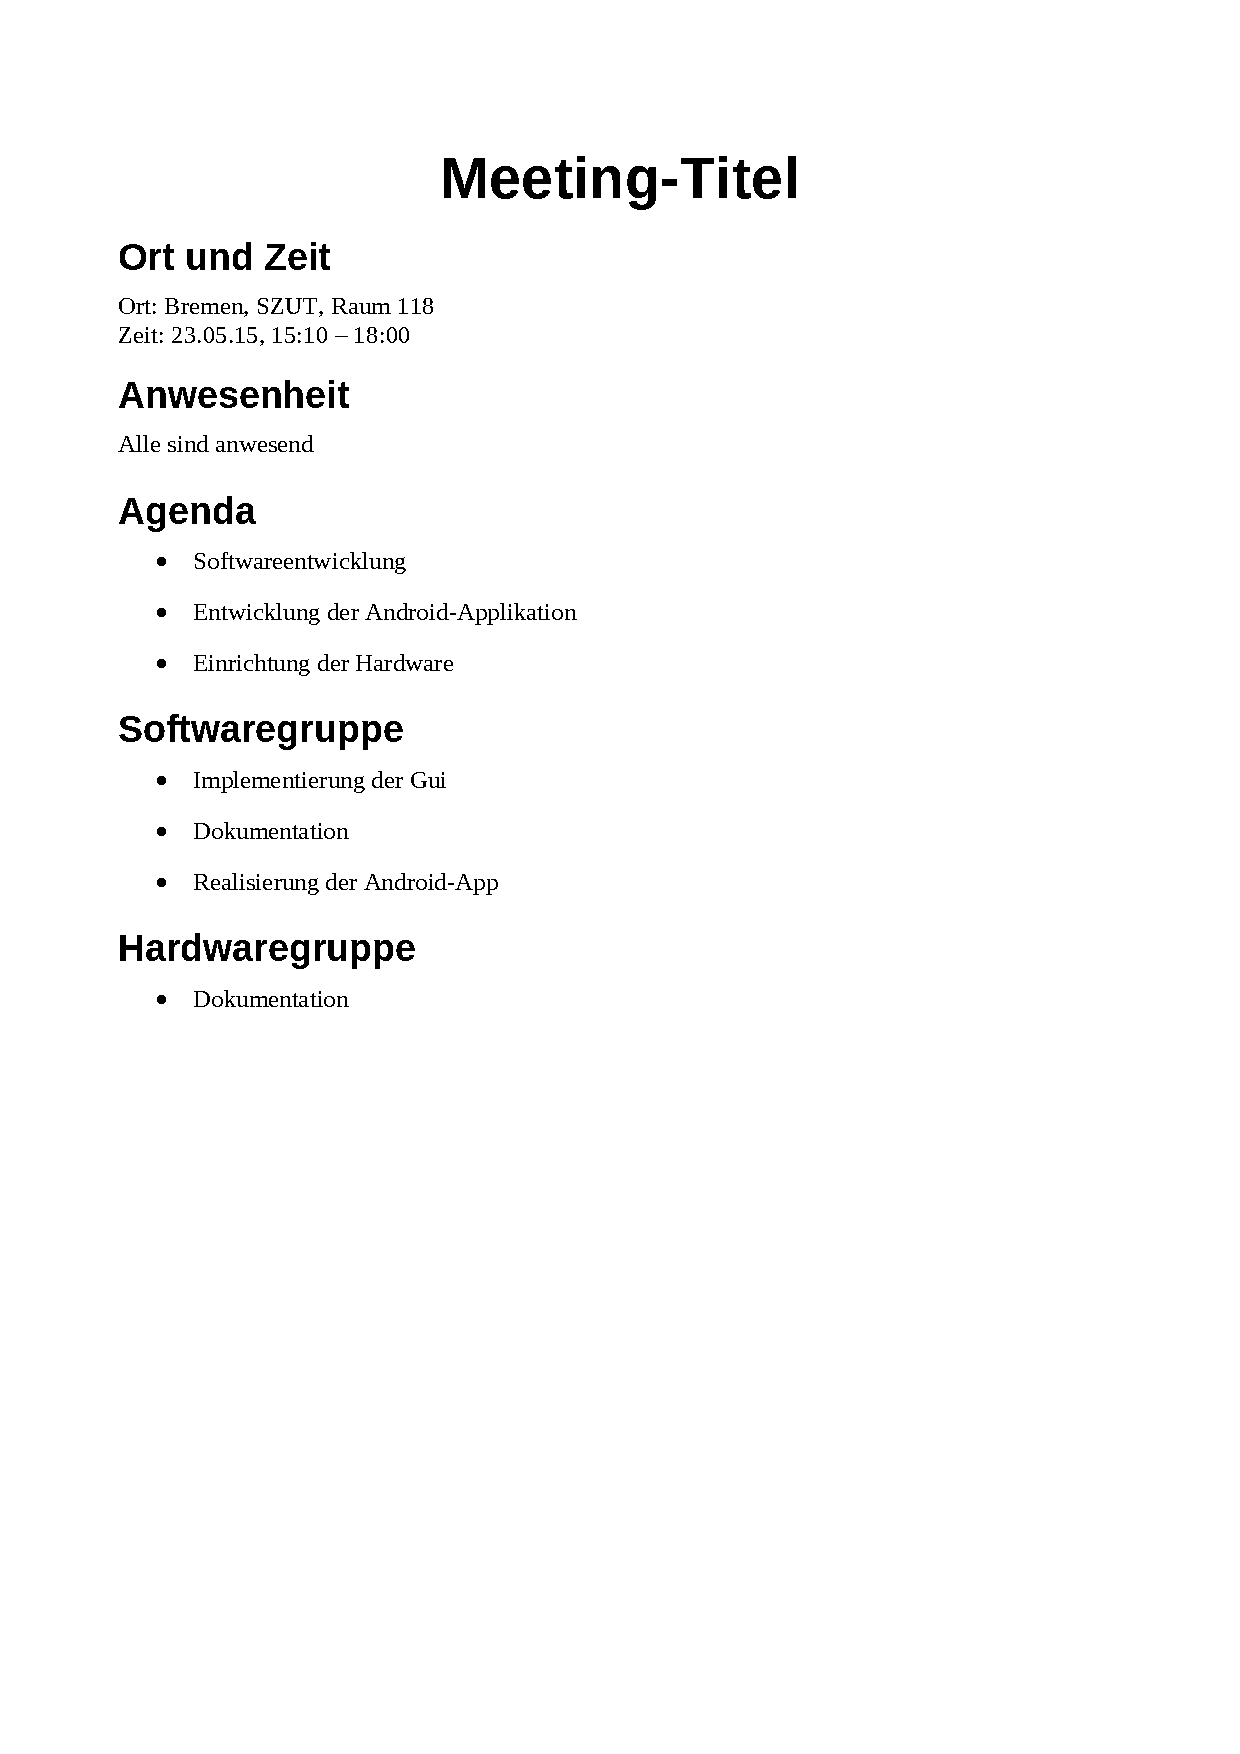
\includepdf{8_Anhang/Protokolle/150412_Meeting_Protokoll}%
\newpage
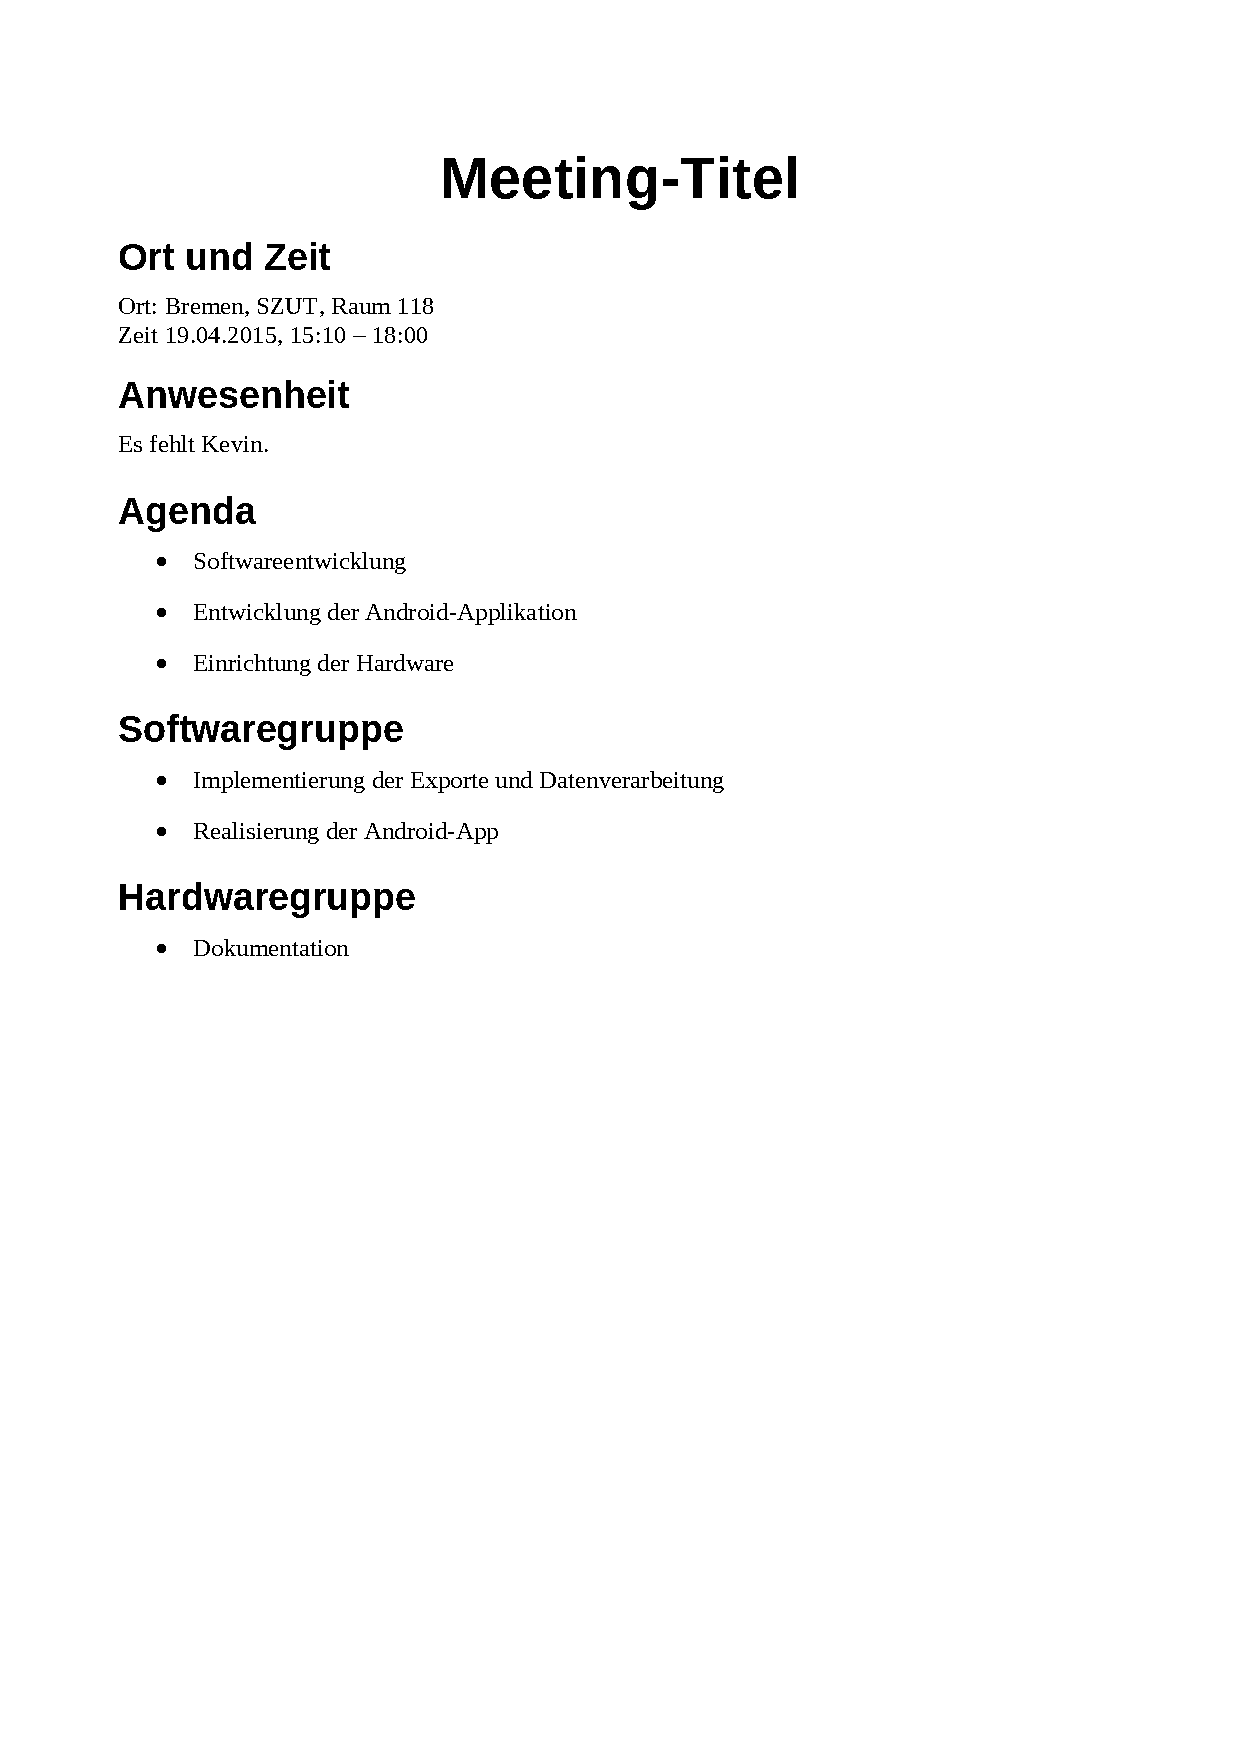
\includepdf{8_Anhang/Protokolle/150419_Meeting_Protokoll}%
\newpage
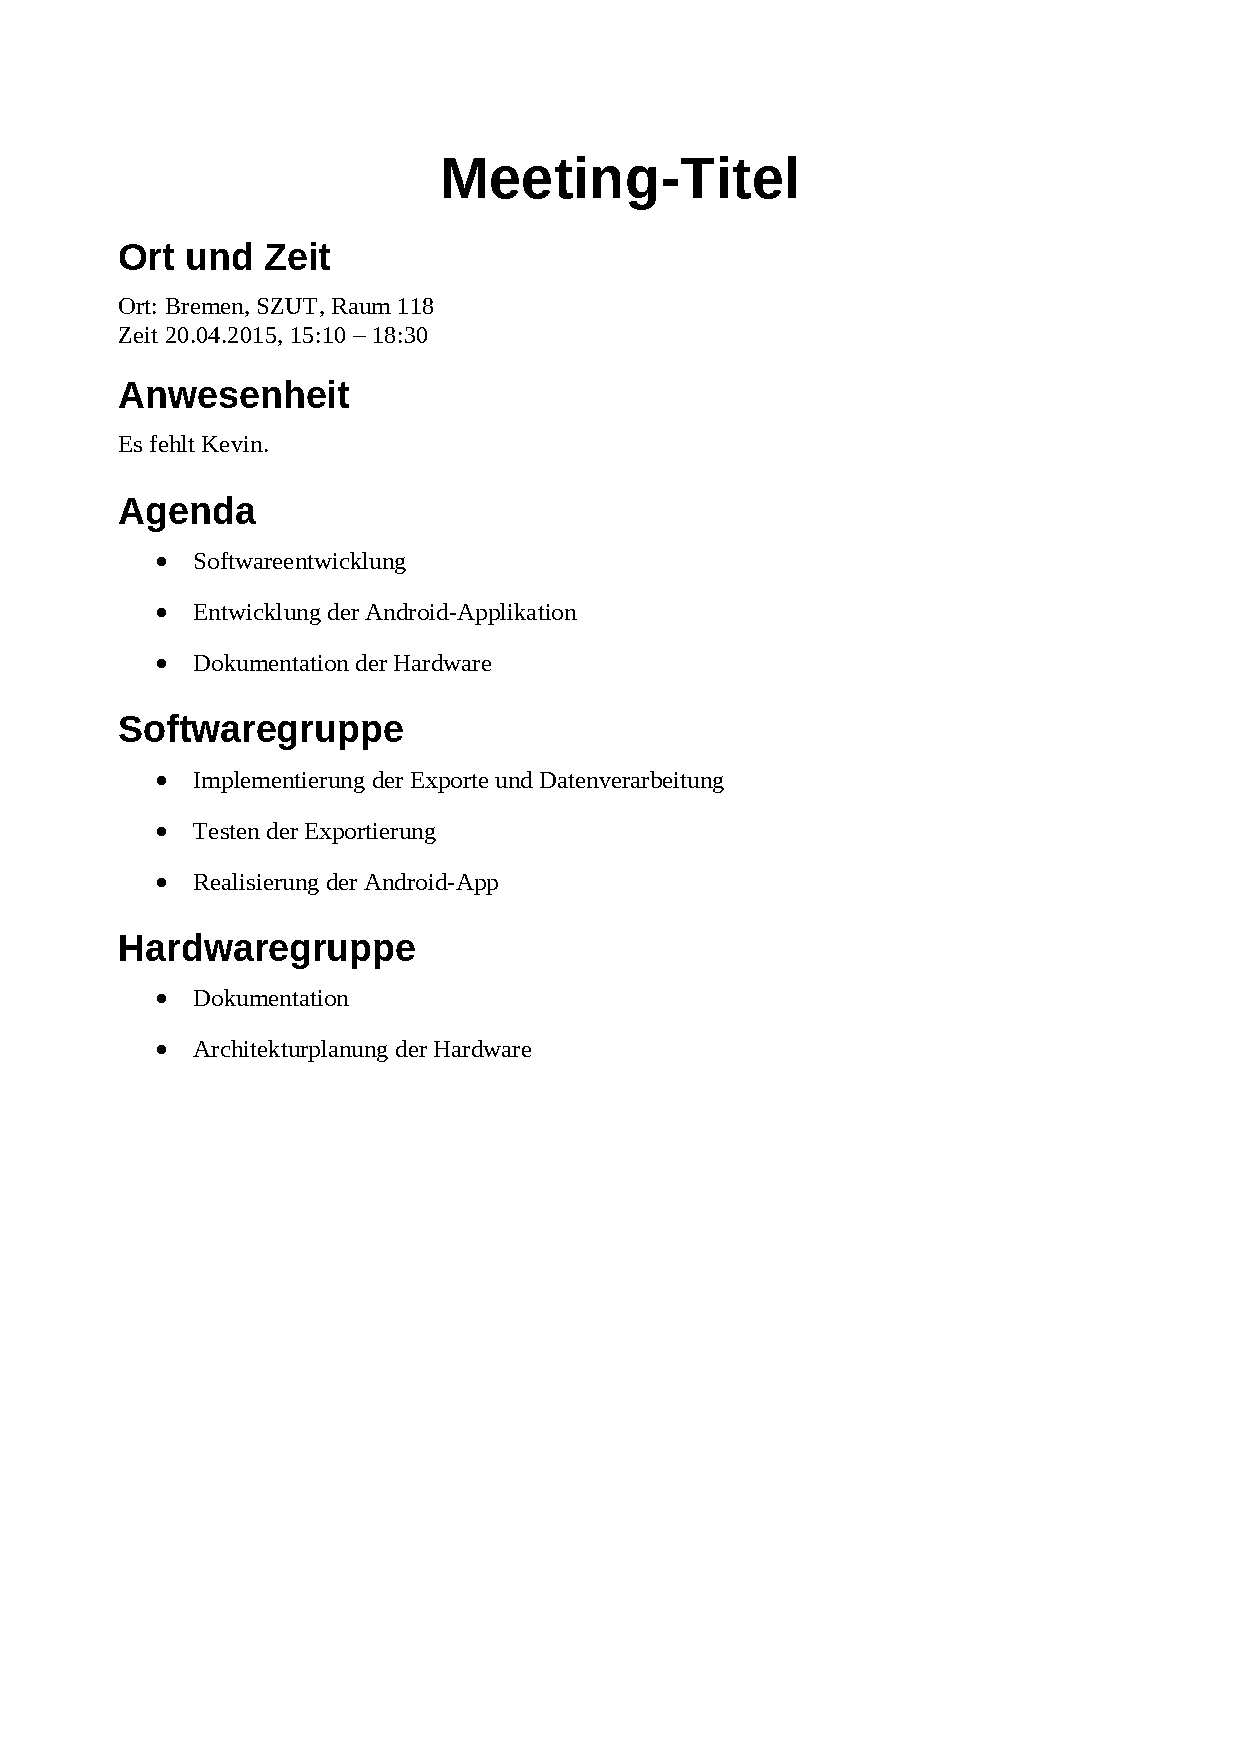
\includepdf{8_Anhang/Protokolle/150420_Meeting_Protokoll}%
\newpage
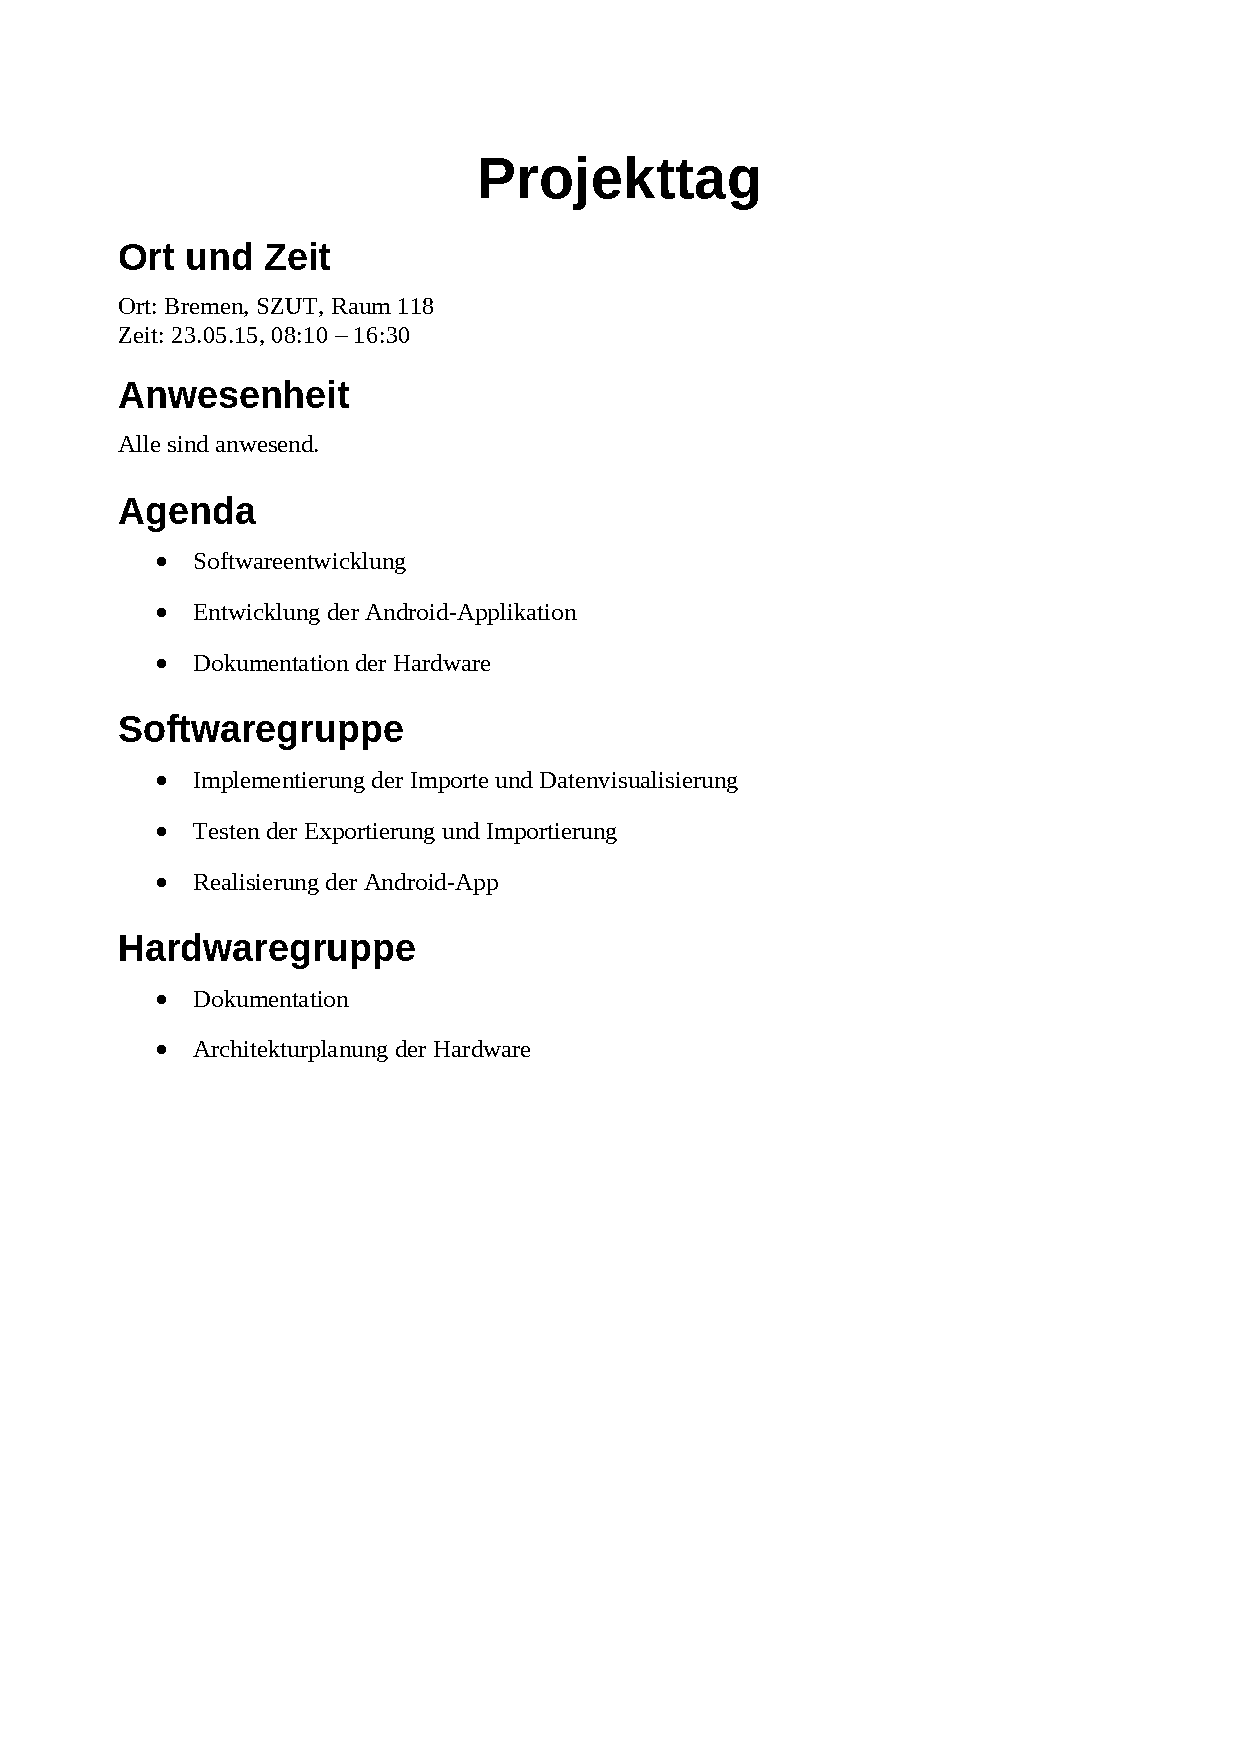
\includepdf{8_Anhang/Protokolle/150426_Meeting_Protokoll}%
\newpage
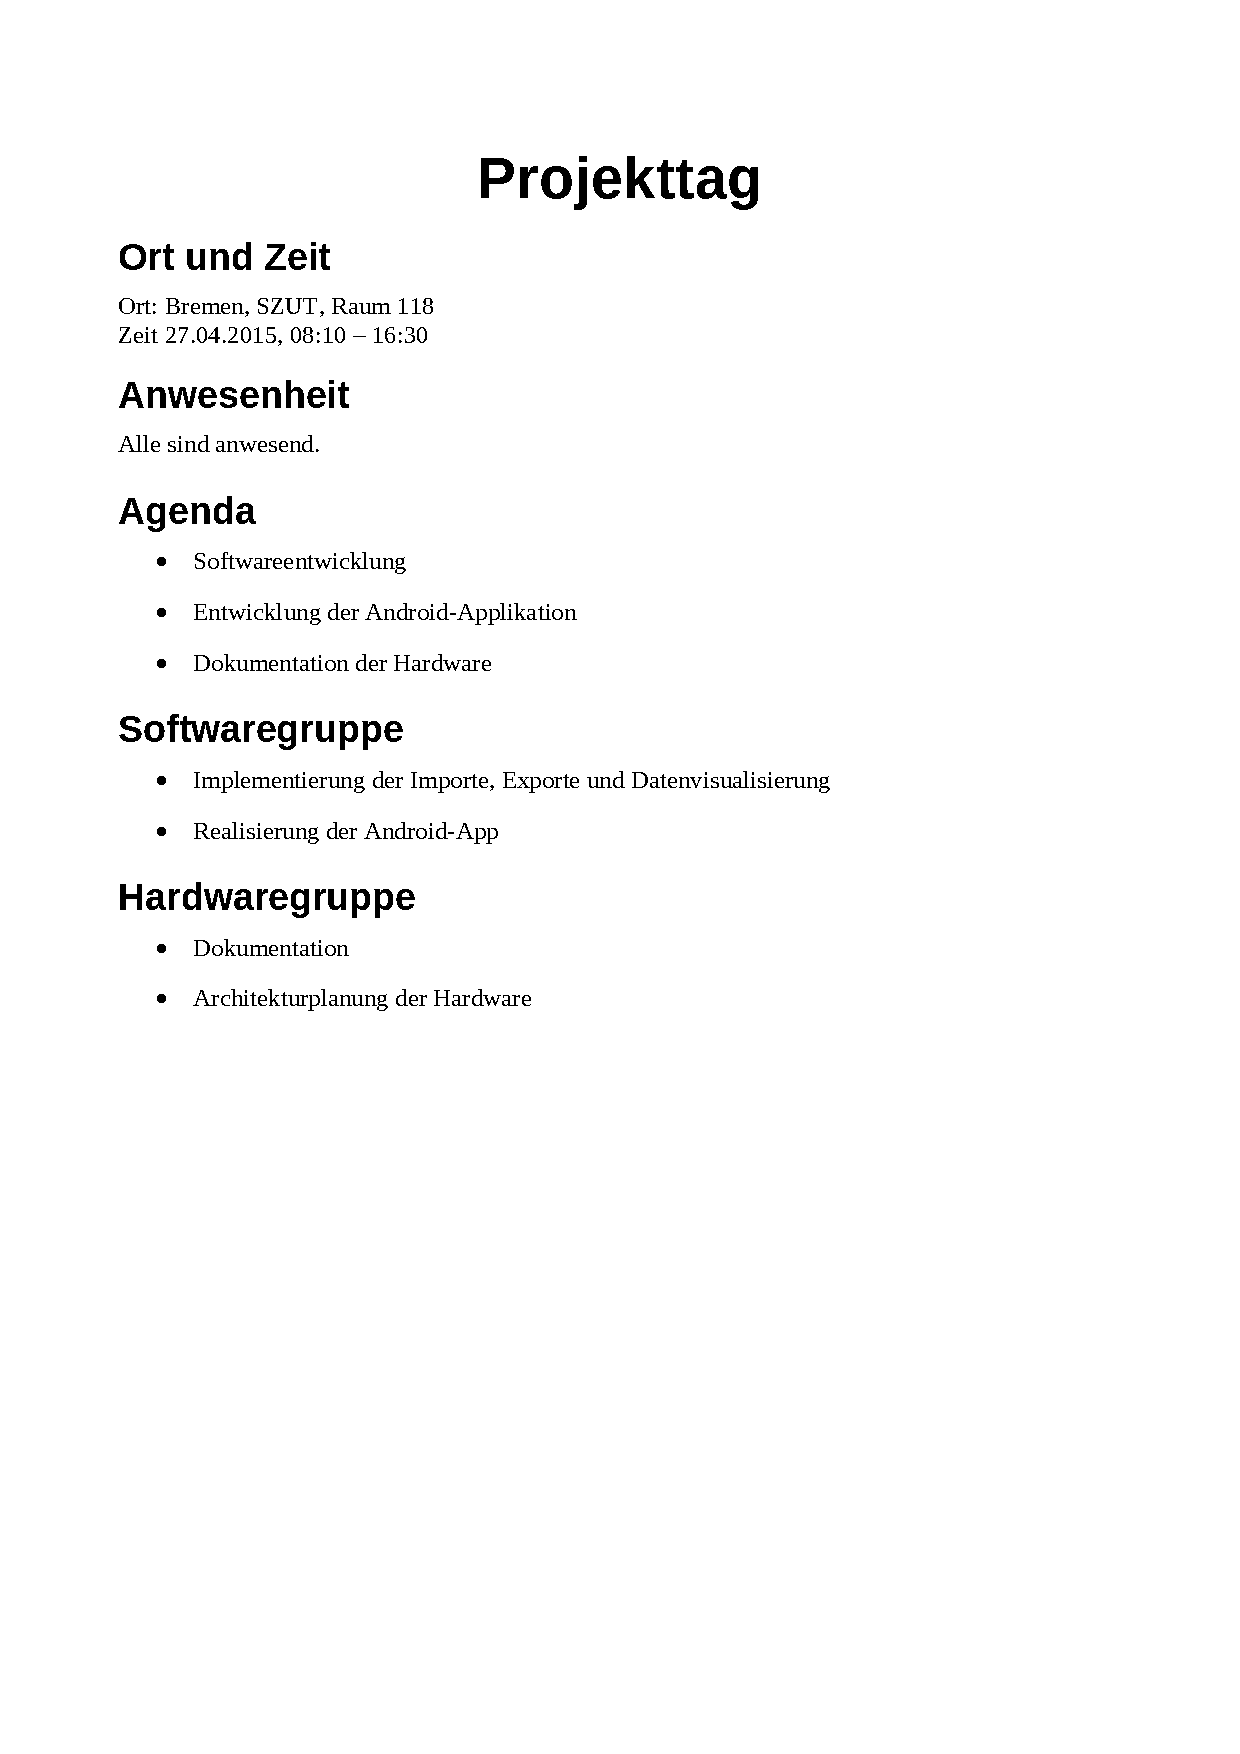
\includepdf{8_Anhang/Protokolle/150427_Meeting_Protokoll}%
\newpage
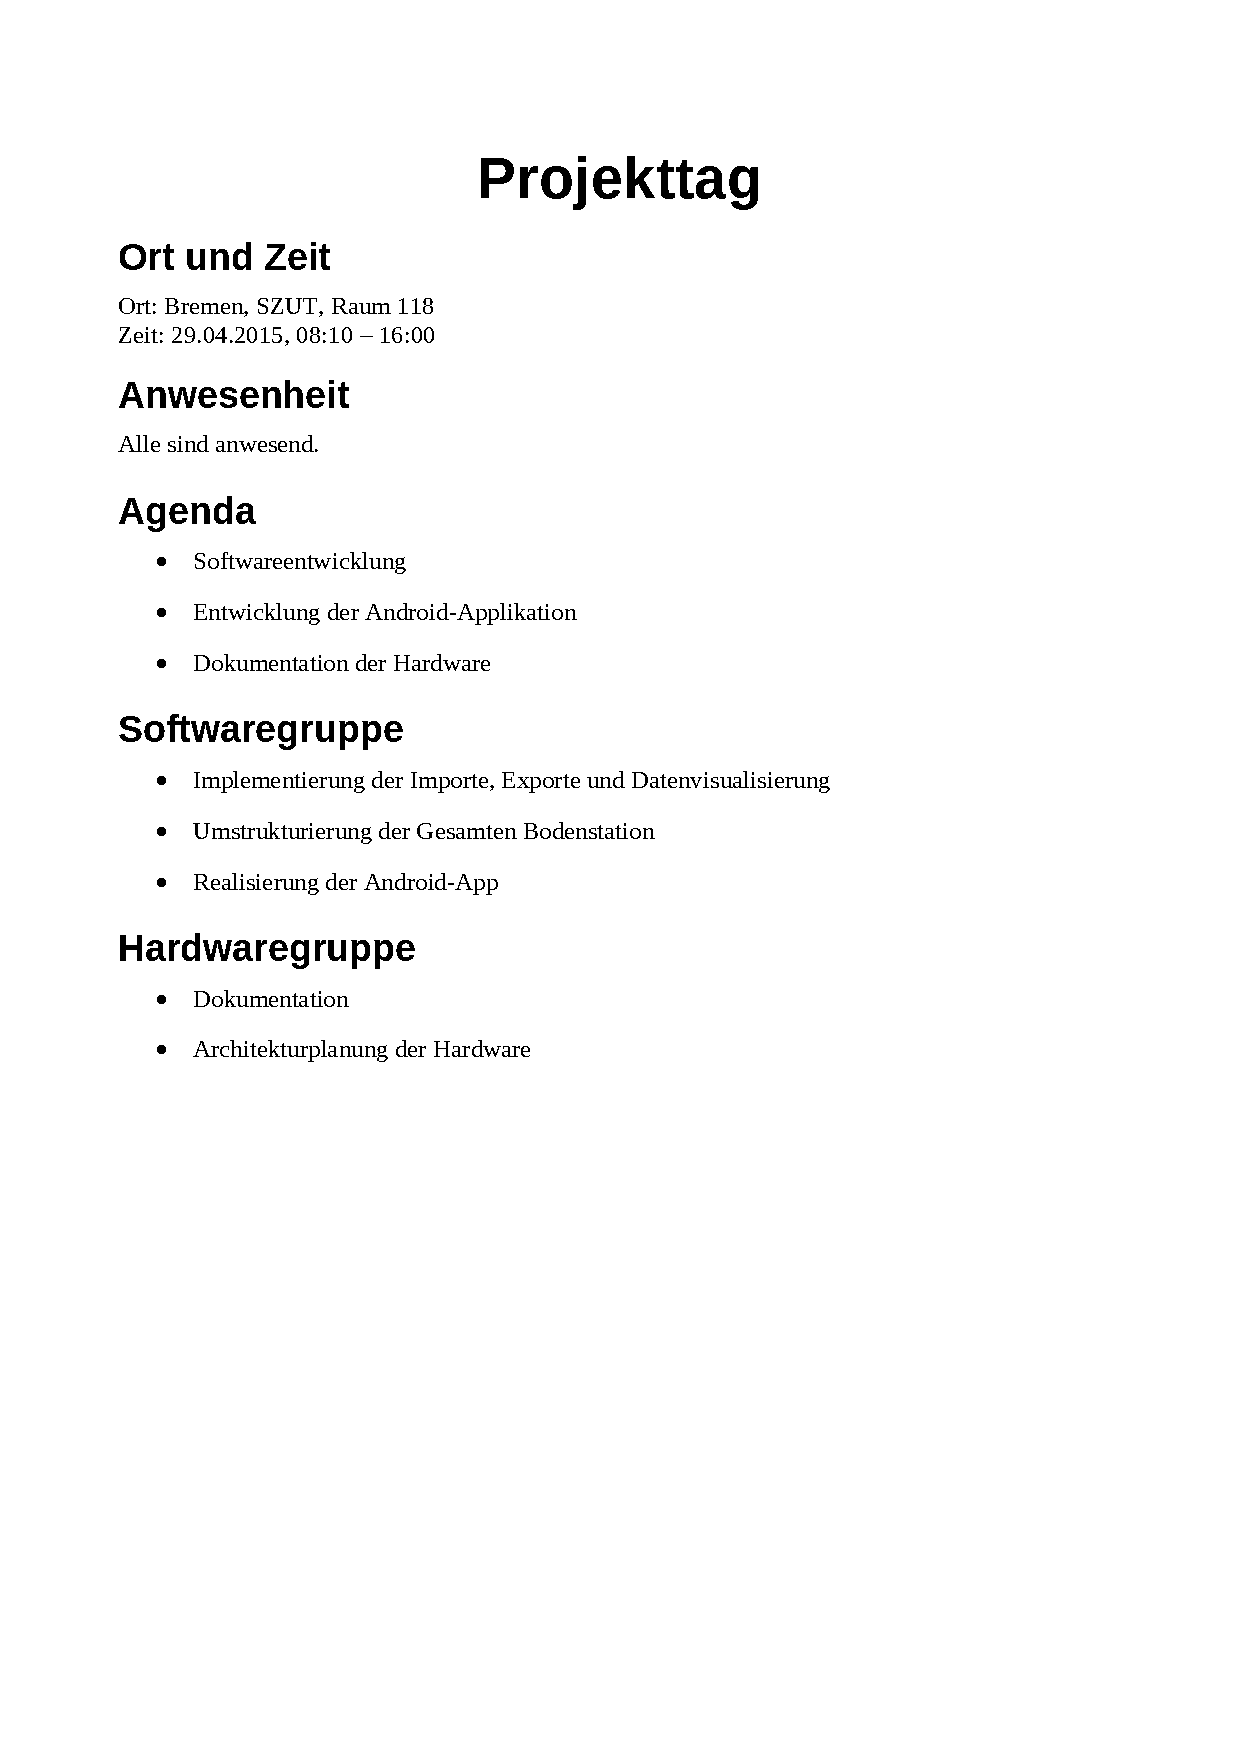
\includepdf{8_Anhang/Protokolle/150429_Meeting_Protokoll}%
\newpage
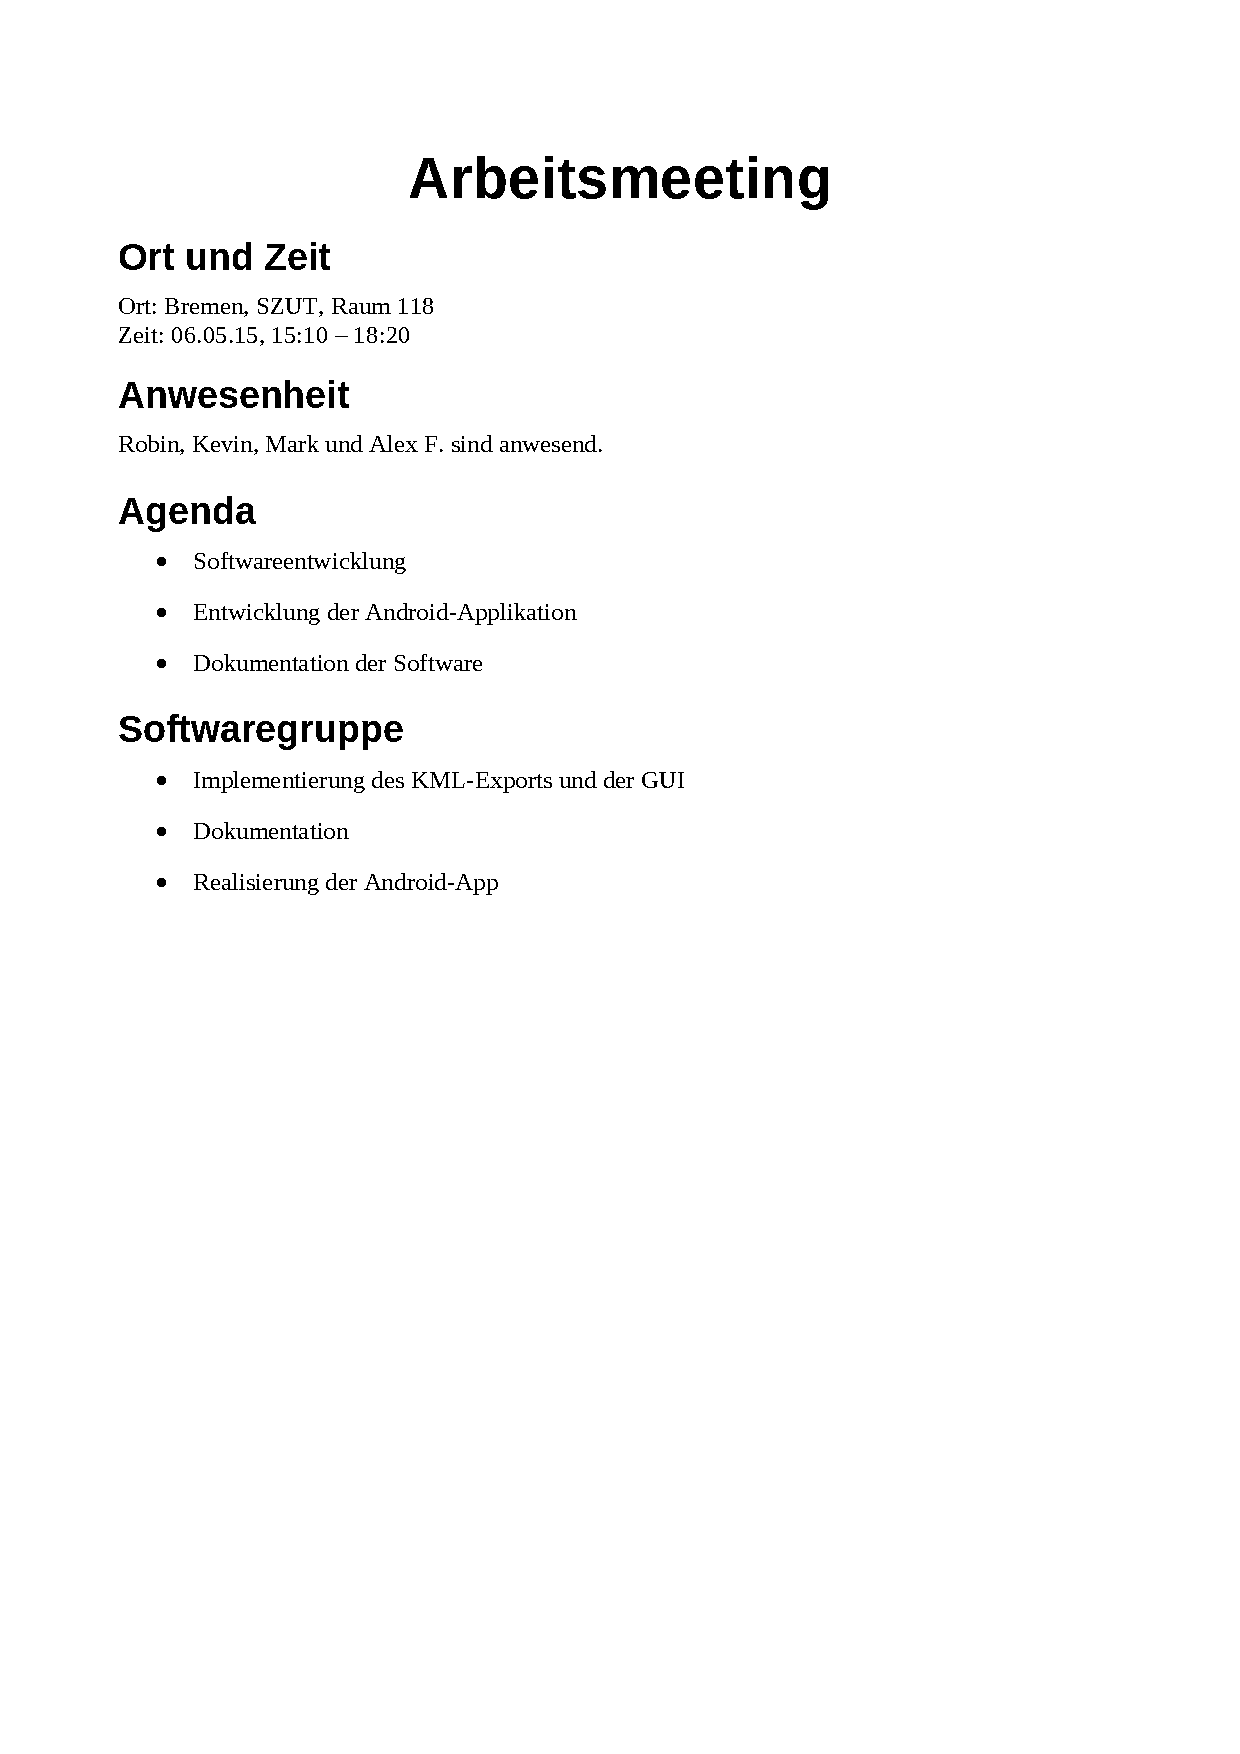
\includepdf{8_Anhang/Protokolle/150506_Meeting_Protokoll}%
\newpage
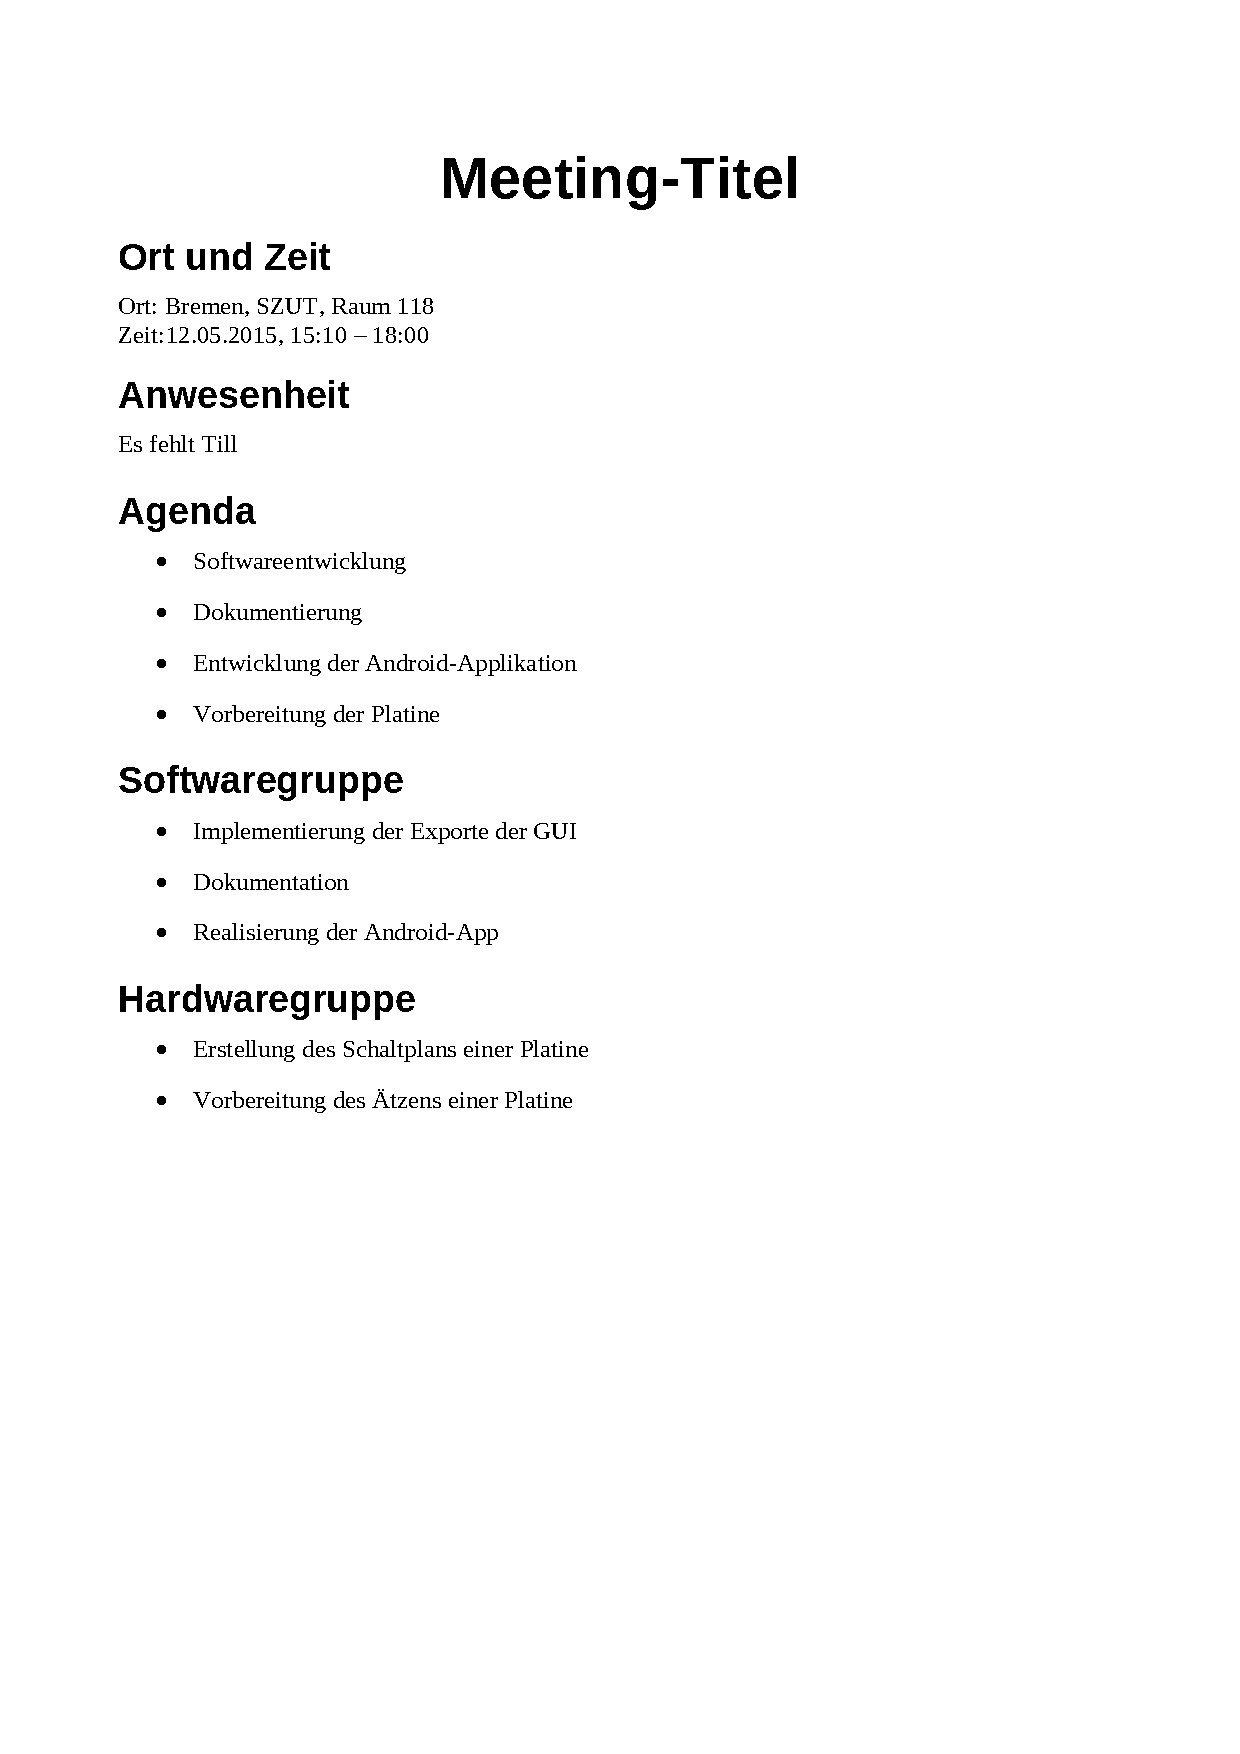
\includepdf{8_Anhang/Protokolle/150512_Meeting_Protokoll}%
\newpage
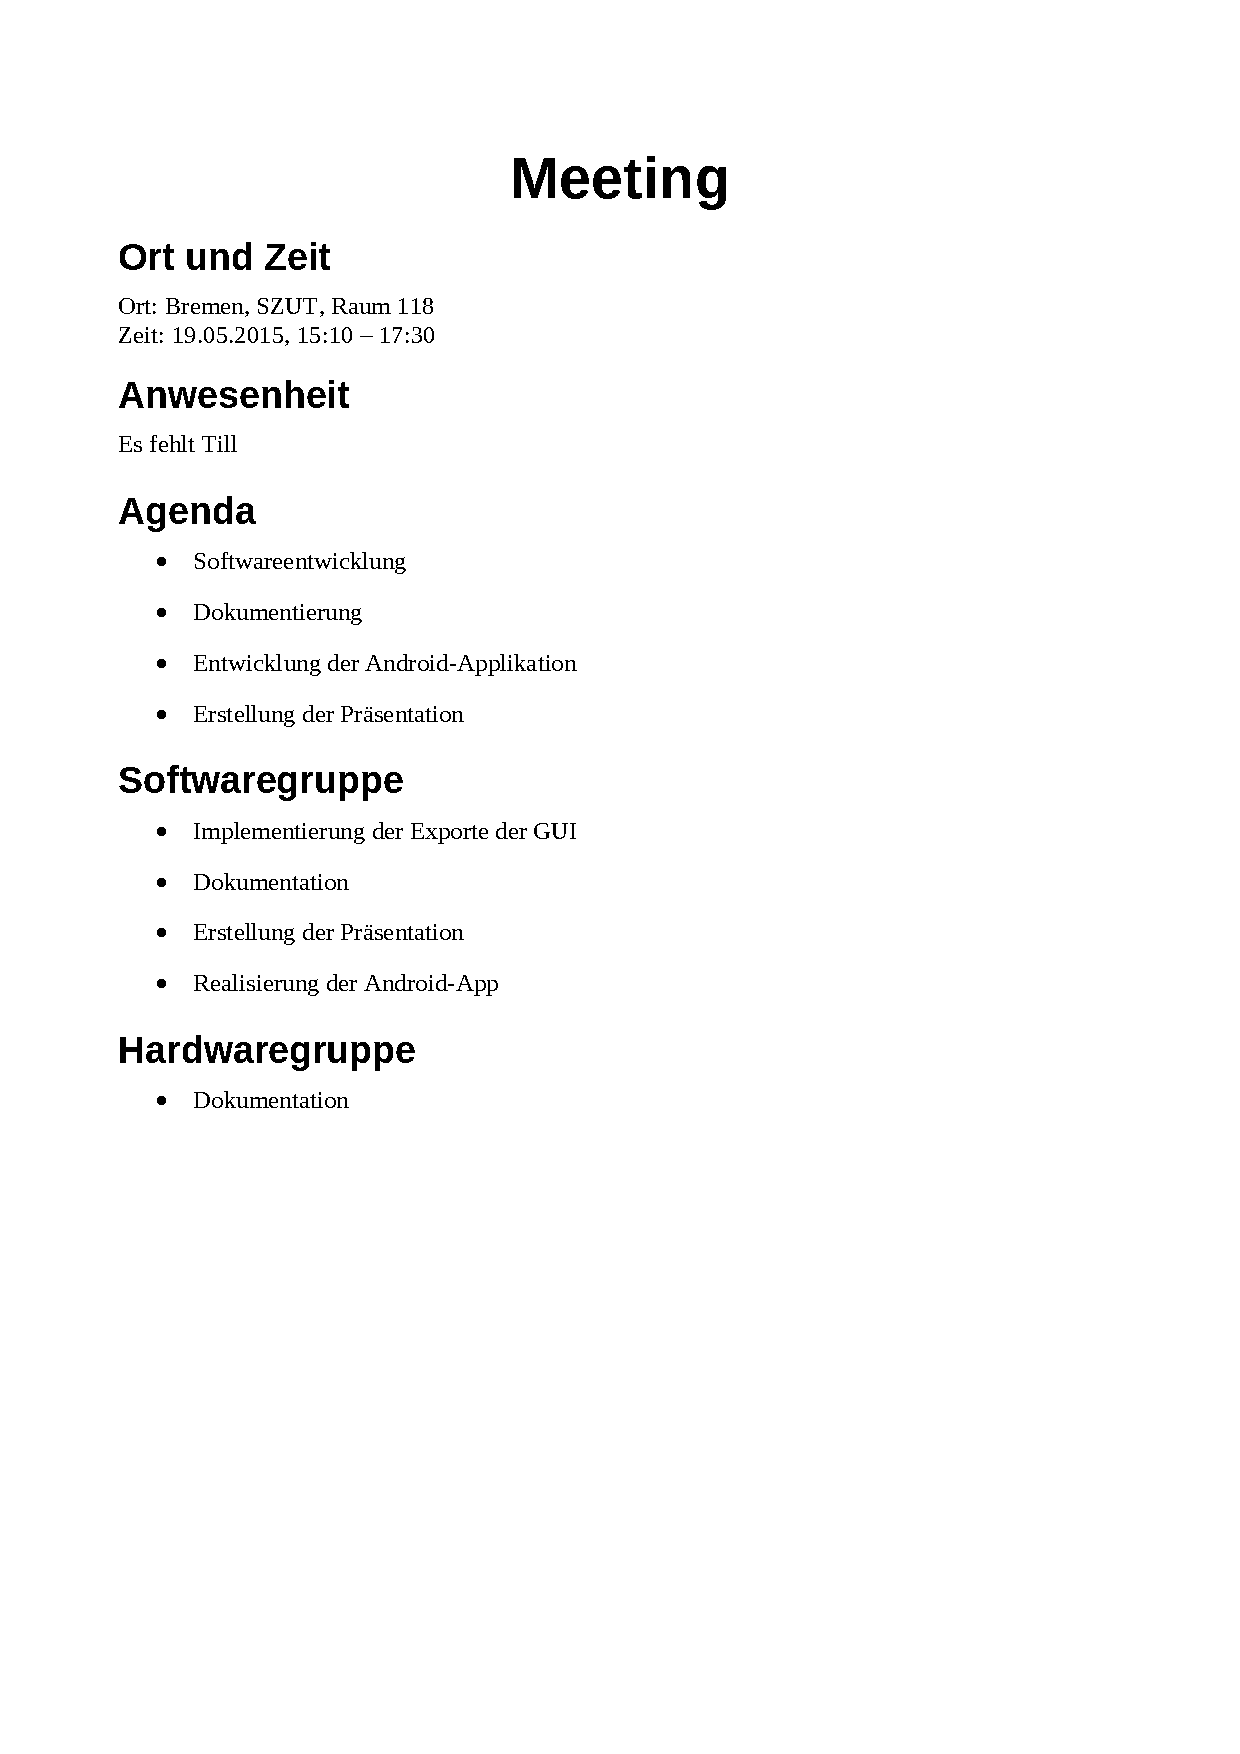
\includepdf{8_Anhang/Protokolle/150520_Meeting_Protokoll}%

\begin{comment}
0

{140921,141022,141202,141203,150106,150204,150210,150217,150303,150310,150317,150412,150419,150420,150426,150429,150506,150512,150520,150522} {

\foreach \i in {00, ..., 999999}%
    \edef\FileName{\i\_Meeting\_Protokoll}%     The % here are necessary to eliminate any
    \FileName%
    \IfFileExists{\FileName}{%  spurious spaces that may get inserted
    \includepdf[width=0.8\textwidth]{8_Anhang/Protokolle/\FileName}%
}%
}%

\end{comment}



\end{document}